\documentclass[12pt,a5paper,twoside]{scrbook}
\usepackage[ngerman]{babel}
%Schrift Quattrocento
\usepackage{quattrocento}
\usepackage[T1]{fontenc}
%Erlaubt Einsatz von Farbe
\usepackage{color}
%UTF 8
\usepackage[utf8]{inputenc}
%Schweizer Anführungszeichen
\usepackage[german=swiss]{csquotes}
%Ermöglicht Zierkapitälchen zum Anbsatzanfang
\usepackage{lettrine}
%Fourier Ornamente für Seitenkopf
\usepackage{fourier-orns}
%Ums Seitenkopf zu manipulieren
\usepackage{scrpage2} 
\pagestyle{scrheadings} 
%Auf jeder Seite ausser Kapitelanfängen oben Linie mit zwei Zeichen in der Mitte
\chead{\color{red}\hrulefill\hspace{0.2cm} \floweroneleft\floweroneright \hspace{0.2cm} \hrulefill}
%Kapitelüberschriften in Schriftart des Deckblatts
\addtokomafont{chapter}{\color{red}\rmfamily\Huge\centering\itshape}
%Schriftart für grosse Anfangsbuchstaben
\input Zallman.fd
\renewcommand{\LettrineFontHook}{\usefont{U}{Zallman}{xl}{n}}
%Schrift für Überschriften
\def\FontH{\fontsize{10pt}{0mm}\usefont{T1}{frc}{m}{n}}
%Bilder einbinden
\usepackage{graphicx}
%Bilder auf ganze Seite ausdehnen
\usepackage{afterpage}
%Bilder von Text umfliessen lassen
\usepackage[vflt]{floatflt} %vflt=ungerade Seitenzahl Bild rechts und v.v.)
%Für Kapitel Gespenst Jonathan Rahmen ermöglichen
\usepackage[everyline=true]{mdframed}
%Definition Rahmen: links dicker roter balken
\mdfdefinestyle{mystyle}{
        roundcorner=10pt,
        backgroundcolor= red!05, 
        bottomline=false,
        rightline=false,
        linewidth=1pt,
        linecolor =red}
\mdfsetup{
%
frametitle={
%
\tikz[baseline=(current bounding box.east),
outer sep =0pt]
\node[anchor=east,rectangle,fill=red]
{\color{white} \small Olivia};},
frametitleaboveskip=\dimexpr-\ht\strutbox\relax
}
\usepackage{tikz} % used for the 'logo' und 
%Delphin zeichnen in Nina
\usetikzlibrary{svg.path}
\newcommand{\Dolphin}[1][]{%
    \tikz \fill [scale=1ex/500,yscale=-1,#1] svg "M 240,792 C 236.7964,782.29301 227.32595,769.18429 218.95458,762.8695 C 210.58318,756.55478 193.07658,741.91749 180.05096,730.34232 L 156.36806,709.29648 L 141.17601,721.53827 C 132.82037,728.27131 116.86485,736.20204 105.71929,739.16215 C 94.57372,742.12228 76.825609,750.15889 66.279001,757.02126 C 42.749986,772.33104 35.286663,768.91329 39.793018,744.89235 C 49.786747,691.62137 86.56609,637.47901 123.0161,622.38091 C 133.32885,618.10921 138.97291,610.6592 143.54681,595.28094 C 156.31386,552.35575 185.13223,485.10659 210.50659,439.02657 C 285.62548,302.61033 377.12604,221.91941 502.90248,181.17368 L 545.4538,167.38902 L 523.9559,153.16241 C 512.13201,145.33777 493.01385,137.67119 481.47106,136.12559 C 441.72739,130.80384 454.06939,100.38528 495.97229,100.38528 C 525.1625,100.38528 588.32595,117.28333 612.47161,131.55225 C 631.20187,142.62093 638.05903,143.46536 711.12662,143.70143 C 826.20118,144.07318 875.39668,159.99674 936.18511,216.548 C 957.70508,236.568 977.32088,249.47994 997.76359,257.08148 C 1037.1384,271.7229 1050.5601,280.83354 1050.5601,292.92001 C 1050.5601,304.96929 1043.1872,306.72156 979.27795,309.86153 C 937.41314,311.91844 922.54209,315.36478 870.35529,335.10414 C 837.1142,347.67736 806.21965,359.09969 801.70072,360.48707 C 797.18181,361.87448 788.5903,373.11962 782.60856,385.47631 C 769.33352,412.89887 732.8923,450.74636 708.71893,462.21739 C 687.47223,472.29962 645.39097,477.58347 636.22902,471.31951 C 626.59388,464.73198 633.77941,451.7414 651.00501,444.60631 C 668.76327,437.2506 688.54805,412.99772 693.73219,392.22992 L 697.39133,377.57125 L 659.92998,381.16743 C 639.32621,383.14537 594.48504,391.40641 560.28293,399.5254 C 408.28252,435.60753 289.59011,503.28314 223.04114,591.81285 L 199.83212,622.68772 L 222.77838,652.2359 C 249.05732,686.07569 265.30365,731.48301 265.30365,771.09095 C 265.30365,810.05728 250.10447,822.61677 240,792 M 885.93164,242.20228 C 889.77822,235.9783 875.83562,229.90601 868.33788,234.5399 C 865.37262,236.37259 864.25805,239.99423 865.8612,242.58811 C 869.72788,248.8446 881.97191,248.60916 885.93164,242.20228 z";%
}
%Abstand zw. Wörtern darf zwecks Blocksatzbildung in Ausnahmefällen bis 1em breit werden.
\setlength{\emergencystretch}{1em}
%bessere Mikrotypographie (margin kerning insb. am Rand)
\usepackage{microtype}
%Seitenzahlen fett
\addtokomafont{pagenumber}{\bfseries}
%To-Do Kommentare einfügen -> \todo{} \missingfigure{}
\usepackage{todonotes}
%Gedichtumgebung
\usepackage{verse}
% Totenkopf
\usepackage{skull}            
%Noten
\usepackage{wasysym}            
%Vogel und Schlange aus Hyroglyphen
\usepackage{hieroglf}            
%Initialen Titelseite (Pseudologo "W")
\input Typocaps.fd
\def\FontI{\color{red}\fontsize{20pt}{0mm}\usefont{U}{Typocaps}{xl}{n}}
%Für Kapitel Schlange werden Longtables benötigt
\usepackage{longtable}
%%%%%%%%%%%%%%%%%%%%%%%%%%%%%%%%%%%%%%%%%%%%%%%%%%%%%%%%%%%%%%%%%%%%%%%%%%%%%%%%%%%%%%%%%%%%%%%%%%%%%%
\begin{document}
%titelseite
\begin{titlepage}
	\begin{center}
		\vspace*{3\baselineskip}
		\FontH{\Huge \color{red} Ein Buch für\\ Linda und Paula}\\ 
	\end{center}
		\vspace*{4\baselineskip}
	
	\begin{center}
		\begin{tabular}{p{7cm}p{5cm}}
			\textbf{\large \color{red} Gordon Wiegand} & \textbf{\large \color{red}  Linda Wiegand}\\
			\textbf{\large \color{red}\itshape Texte} & \textbf{\large \color{red}\itshape Illustrationen}\\
		\end{tabular}

	\end{center}
		\vspace*{4\baselineskip}
	\begin{center}
   		\large\FontI{W}
	\end{center}

\end{titlepage}
%Bild Seite 2
\begin{figure}[ht]
\centering
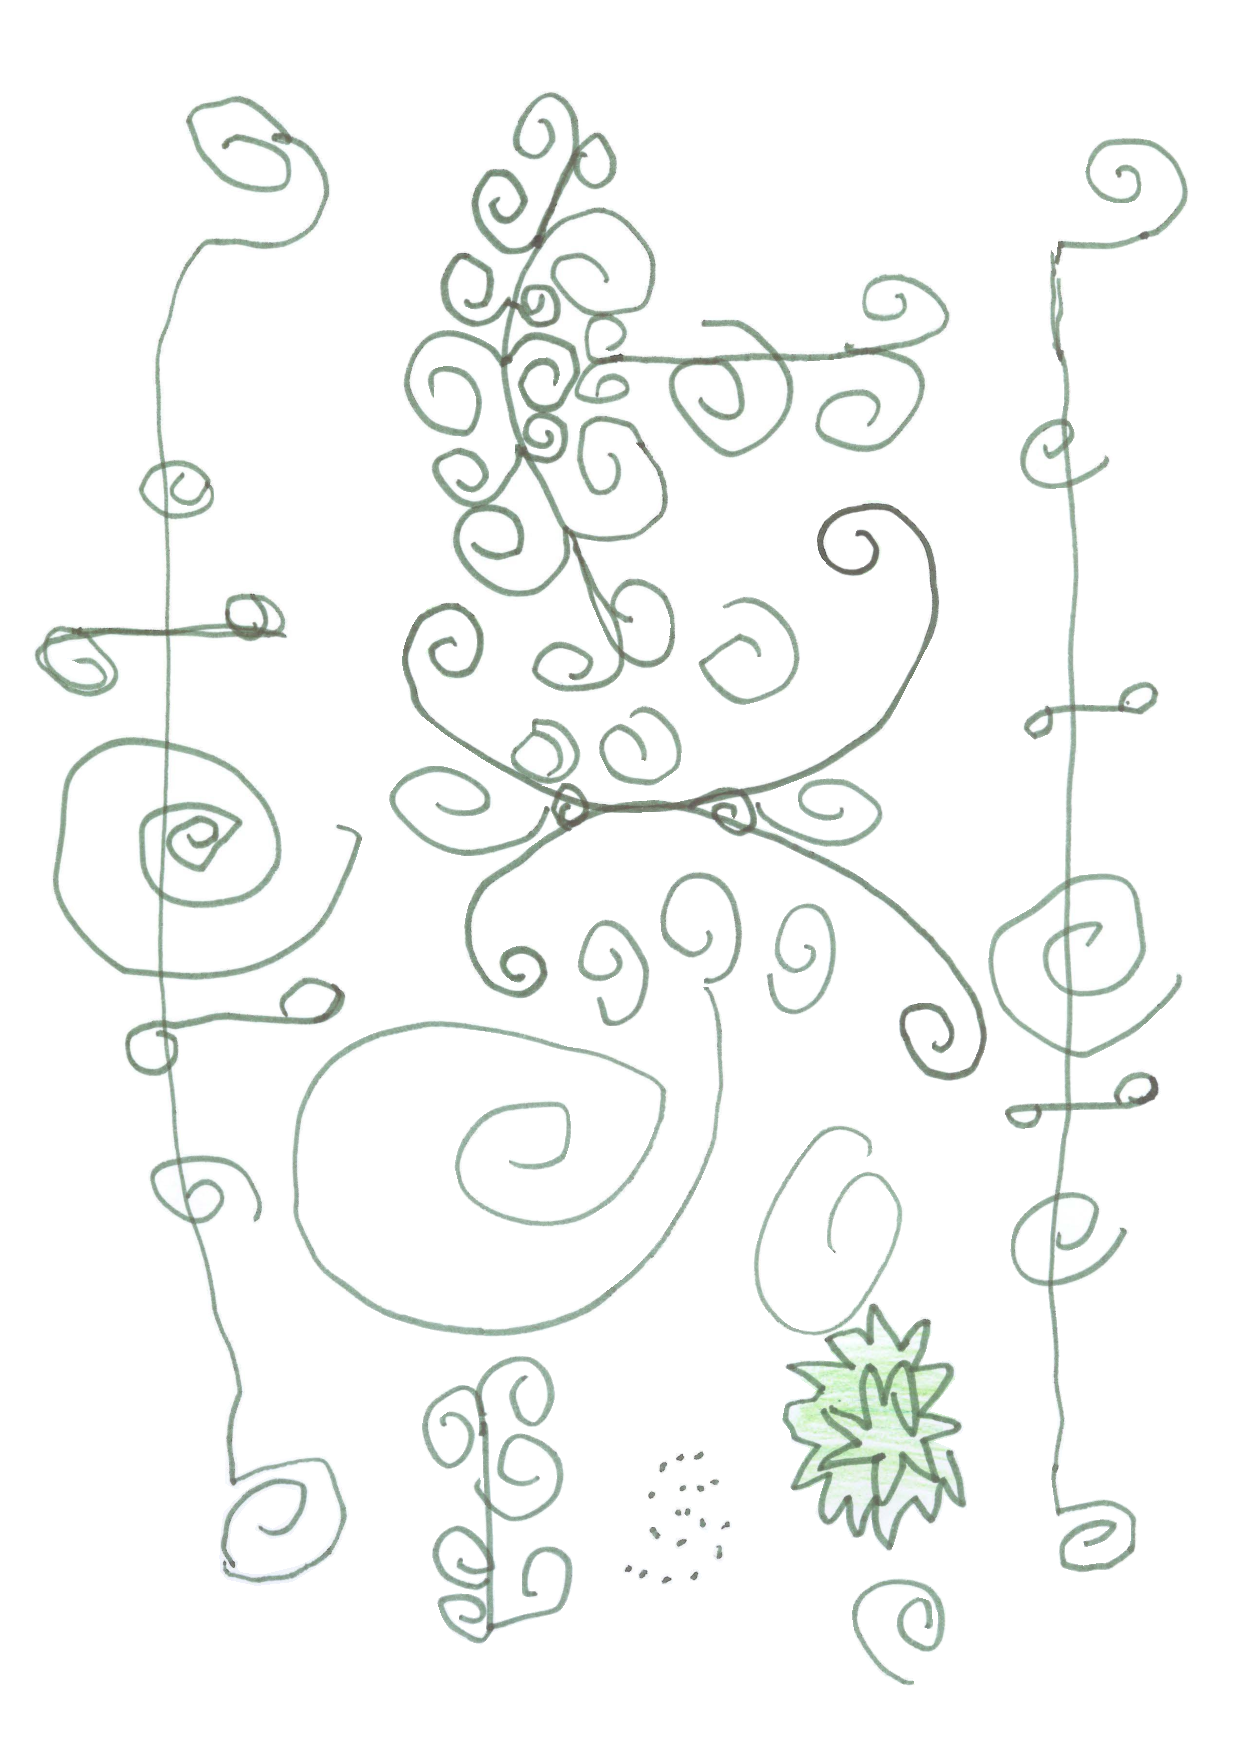
\includegraphics[width=\textwidth]{bilder/titelbild.pdf}
\end{figure}
%Kapitel einfügen
%\chapter*{\FontH{\Huge TBD}}
\addcontentsline{toc}{chapter}{Die Papageieninsel}
%\lettrine[lines=3]{\color{red}E}{inleitung} kommt noch.

\setlength\LTleft{0pt}
\setlength\LTright{0pt}
\begin{longtable}{@{\extracolsep{\fill}}ll}
%\begin{longtable}{ll}
%\textpmhg{D}%Schlange
%\textpmhg{\Hibw}%Vogel
\textpmhg{\Hibw} & Diese Wiese ist mein Reich\\
& Ich bin hier der König\\
& Die Schlange da, die ess ich gleich\\
& Sie ist so zart und butterweich\\
& \\
\textpmhg{D} & Was kommt denn für ein Vogel dort?\\
& So saftig, zart und lecker\\
& 
\end{longtable}
 \hfill {\color{red}\decofourleft}

\chapter*{\FontH{\Huge Tabea Timpetampe und Herr Häusler}}
\addcontentsline{toc}{chapter}{Tabea Timpetampe und Herr Häusler}
\lettrine[lines=3]{\color{red}T}{abea} Timpetampe sitzt im Sandkasten und spielt. Sie hat gerade ein Dach auf ihr Sandhaus gebaut, als ihr einfällt, dass das Dach ja auch nass werden kann, wenn es regnet. Also baut sie noch ein Dach für das Dach. Und für dieses dann auch noch eins und noch eins und noch eins oben drauf.

\enquote{Was machst Du da?} Eine Weinbergschnecke ist auf Tabea Timpetampes Eimerchen geklettert und bestaunt das Bauwerk. 

\enquote{Ich baue eine Burg}, antwortet Tabea Timpetampe, denn sie bemerkt gerade, dass das Dach auf dem Dach eines Daches viel mehr wie ein Turm aussieht. Und Türme gehören zu Burgen. Aber wenn sie schon einmal Besuch hat, kann sie ja eigentlich auch gleich mal eine Pause machen. In einem Döschen hat sie noch Banane von Mama bekommen, die gerade dabei ist, mit ihrer grossen Schwester Fahrradfahren zu üben. 

Die Banane in Stücke zu schneiden ist ja wohl das Dümmste, das kann sie heute gar nicht leiden. Ein Glück, dass Tabea Timpetampe die beste Köchin des Sandkasten ist. Im Nu hat sie eine herrliche Suppe aus Sand und Gras und Blumen gezaubert. Rein mit der Banane und abschmecken. Prima, die knirscht wenigstens zwischen den Zähnen, da kann man auch gleich hören, ob man isst, falls man mal gerade keine Lust hat, zu schmecken.

\enquote{Wenn ich mal gross bin, dürfen meine Kinder immer nur Banane mit Suppe essen.}, erklärt sie der Schnecke. Die streckt nur ihre Fühler gelangweilt in Richtung Sonne. Die Schnecke ist schon alt, schon fast ein Jahr und wenn man so alt ist, mag man den Satz \textit{Wenn ich mal gross bin, dürfen meine Kinder \dots} einfach nicht mehr hören.

\enquote{Ich muss weiter}, erklärt die Schnecke, \enquote{Ich jogge gerade und da darf man nicht kalt werden. Immer in Bewegung bleiben, sonst werden die Muskeln hart.} Und mit einem \textit{Hopp, Hopp, Hopp} joggt sie  davon.

Tabea Timpetampe staunt überhaupt nicht, dass Schnecken joggen. Was sollen die denn sonst für eine Sportart treiben, bitteschön? Ohne Arme kann man kein Federball spielen und ohne Füsse kein Fussball. Da bleibt nur noch das Joggen übrig. 

Sport sei gesund, behauptet Papa. Das behauptet er auch bei Brokkoli und wenn er das Fenster öffnet, obwohl es kalt draussen ist und wenn sie ins Bett soll, obwohl sie noch gar nicht schlafen will. Gesund muss also irgendetwas schlechtes bedeuten, schlussfolgert Tabea Timpetampe nicht ganz richtig, denn Papas haben gewöhnlich immer Recht. Also lieber schnell die Schnecke retten, bevor noch etwas Schlimmes passiert.

Zum Glück ist die Schnecke noch nicht sehr weit gekommen mit ihrem Joggen, gerade will sie nach dem Schäufelchen seitlich abbiegen, da wird sie von Tabea Timpetampe hoch gehoben und auf den Rand des Sandkastens gesetzt -- zur Rettung. 

\enquote{Liebe Frau Schnecke}, fängt sie an zu erklären, wird aber unterbrochen.

\enquote{Ich bin ein Herr und keine Frau und wenn es dir nicht zu viele Umstände macht, ich heisse Herr Häusler. Wir Weinbergschnecken haben ein Häuschen auf dem Rücken und heissen deswegen alle Häusler. Das ist eine Stilfrage. Jedenfalls will ich mit unbehausten Schnecken nicht verwechselt werden. Das nennt man Kultur, das wirst du schon noch lernen, junge Dame.}

\afterpage{
\begin{figure}[h]
    \vspace{5cm}
\centering
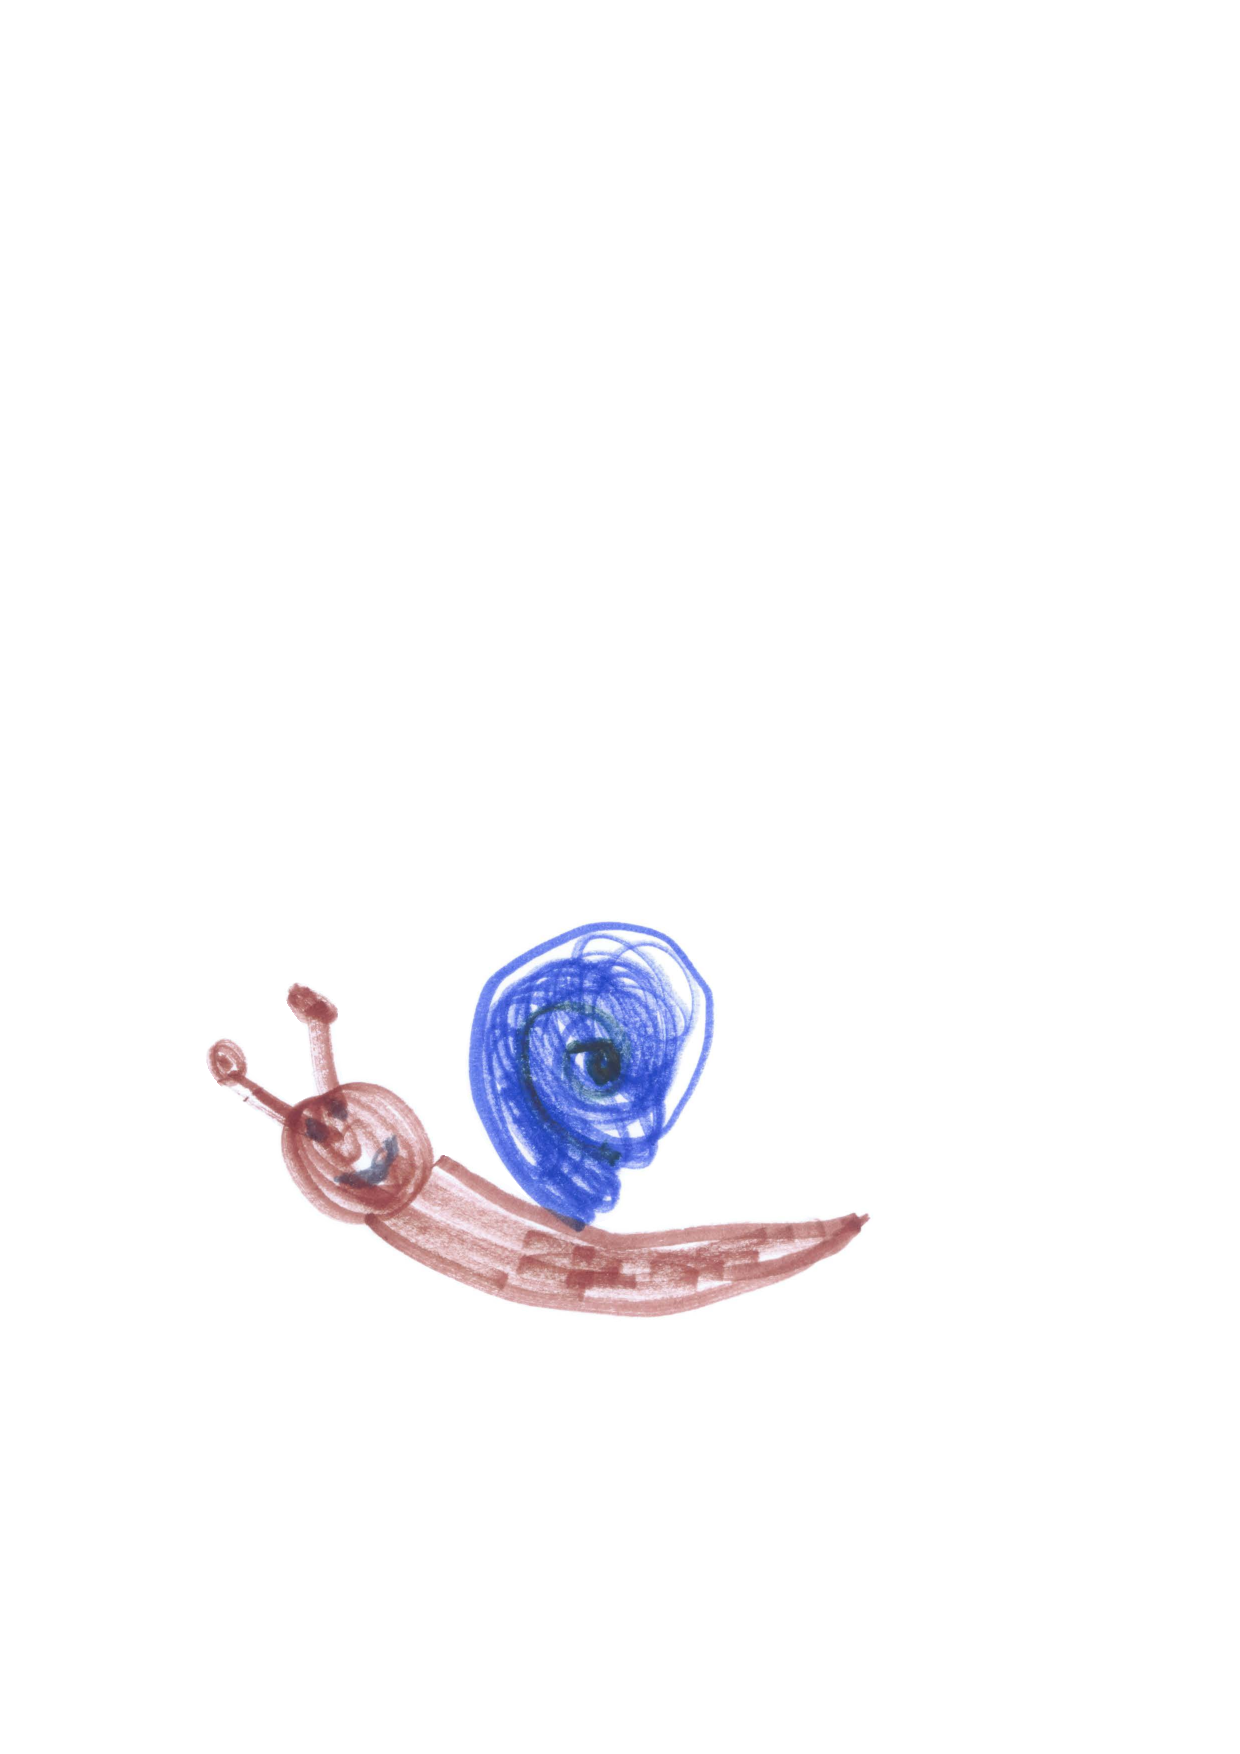
\includegraphics[width=\textwidth]{bilder/1schnecke.pdf}
\end{figure}
\clearpage
}

Aha, denkt Tabea Timpetampe. Eine sehr vornehme Schnecke. Gerade wie eine Prinzessin aus einem Märchen. Sie nimmt Herrn Häusler und setzt ihn in die Sandburg.

\enquote{Bitteschön!, Ihre eigene Burg.}, erklärt sie. Herr Häusler wird sichtbar grösser vor Stolz. Eine eigene Burg ist besser als Joggen, so viel wäre auch der dümmsten Schnecke klar gewesen. Sie spielen eine Weile zusammen. Herr Häusler ist die Prinzessin und Tabea Timpetampe die Baumeisterin. Herr Häusler lässt sich auch bereitwillig ein Kleid aus einem grossen Kastanienblatt basteln, in das er immer mal hinein beisst, wenn Tabea Timpetampe gerade nicht guckt. Vermutlich ist es ja unhöflich, ein Kleid, das man gerade bekommen hat, aufzuessen. Ganz sicher ist sich Herr Häusler auch nicht immer in Stilfragen.

Sie bauen noch eine Höhle und eine Strasse und verstecken einen Schatz in der Ecke des Sandkastens. Einen gestreiften Stein. Tabea Timpetampe ist zufällig grosse Expertin, wenn es um das Finden besonderer Steine geht. Im Wintergarten zwischen den Blumentöpfen liegt schon eine beachtliche Sammlung. Mama hat neulich sogar vorgeschlagen, dass Tabea Timpetampe alle Steine in einen echten Schuhkarton legen darf. Die weiss das also auch zu schätzen.

\enquote{Das ist jetzt unser Geheimnis.}, entscheidet Tabea Timpetampe und da kann Herr Häusler nur zustimmen. 

Ein grosses Weinen beginnt, denn Tabea Timpetampes Schwester ist umgefallen. Die Mama tupft an der Wunde herum und jetzt schnell nach Hause, heisst es. Tabea Timpetampe kann Mama gar nicht Herrn Häusler vorstellen, sie darf sich nicht einmal verabschieden. Sie wird -- zack -- von Mama am Arm genommen und ab geht es. So unbeachtet zu bleiben, gefällt Tabea Timpetampe überhaupt nicht, da weint sie lieber auch gleich mit.

Am nächsten Tag darf Tabea Timpetampe nicht im Sandkasten spielen, denn es regnet. Am Tag darauf werden die Grosseltern besucht und es ist noch irgendetwas, dass sie nicht so ganz genau verstanden hat. Aber es klappt wieder nicht, draussen zu spielen. Dabei hat sie doch so grosse Lust, Herrn Häusler wiederzusehen. 

Am Wochenende ist es endlich so weit. Aber Herr Häusler ist nicht mehr da. Natürlich nicht, so lange wartet ja niemand. Tabea Timpetampe ist sehr traurig und sucht überall. Vielleicht joggt er ja irgendwo auf der Wiese? Aber nichts. Weit und breit keine Schnecke. Bestimmt hat Herr Häusler sie längst vergessen. Sie mag gar nichts spielen.

Dann fällt Tabea Timpetampe der Schatz wieder ein. Sie sieht nach. Der Schatz ist noch da, aber es ist noch etwas dazu gekommen: ein Schneckenhaus, von Herrn Häusler, für sie. Da hat Tabea Timpetampe wieder Lust zu spielen. Sie baut die Burg wieder neu und die Strasse und die Höhle. Alles sogar noch ein bisschen grösser als das letzte Mal. Und sie vergräbt den Schatz neu, aber ohne das Schneckenhäuschen, das nimmt sie lieber mit nach Hause. \hfill {\color{red}\decofourleft}

\chapter*{\FontH{\Huge Löwenalarm}}
\addcontentsline{toc}{chapter}{Löwenalarm}
\lettrine[lines=3]{\color{DeepPink}M}{ama} und Papa schlafen noch. Mama wie üblich etwas lauter als Papa.  Sehr wohlig klingt das. Ich hatte mich zwar erst auch noch zu ihnen gelegt, aber das war diesmal doch zu langweilig, lieber gleich wach bleiben. 

Der aufregendste Ort bei mir zuhause ist die oberste Schublade im Schreibtisch von Mama. Eigentlich darf ich die gar nicht aufmachen, denn dort gibt es auch eine Schere und Reisszwecken und allerhand andere Dinge, die für mich gefährlich sein könnten. Behaupten jedenfalls Mama und Papa und die sagen, dass man mindestens sechs Jahre alt sein muss, um da aufmachen zu dürfen. Aber ich kann ja spielen, ich sei schon so alt. 

Tausend Dinge gibt es in dieser Schublade. Bei den meisten weiss ich gar nicht, wozu die gut sind. Zum Spielen sind sie jedenfalls prima geeignet. Eine Dose mit kleinen silbernen Dingern geht erst nicht auf, dann purzeln alle auf den Boden. Ein Lineal kommt zum Vorschein, das kenne ich schon. Eine 1A-Rutschbahn gibt das Lineal, wenn man es schräg hält. Nach und nach dürfen alle Schubladenbewohner die Rutsche einmal ausprobieren. Wer vor dem Ende abstürzt ist blöd. 

Ganz hinten in der Schublade entdecke ich einen Stift, den ich noch nie gesehen habe. Der ist ganz dick und bunt. Aha, wenn man hier drückt, kann man rot schreiben und wenn man hier drückt blau. Gelb und Schwarz gibt es auch und Rosa -- meine Lieblingsfarbe -- ist auch dabei.

Zum Stift fehlt noch Papier, das liegt im Arbeitszimmer. Da kann ich gleich noch auf dem Stuhl im Kreis drehen und spielen, dass ich Rennauto fahre. Aber zuerst Malen. 

Der erste Strich ist rosa. Die Farbe passt ja wohl nur zu Feen, also fange ich an, eine Fee zu malen. Erst eine grosse Fee, dann noch eine und dann noch drei kleine dazu. Eine Feenfamilie mit zwei Mamas. Aus dem Schlafzimmer höre ich \emph{meine} Mama immer noch schnarchen. Wie ein Löwe klingt das, also male ich auch noch einen Löwen. Der bekommt eine grosse Mähne aus Kringeln und einen aufgerissenen Mund. Der Löwe brüllt nämlich gerade. Und spitze Zähne hat der auch, die muss man ganz vorsichtig malen, die sind gefährlich!

Und jetzt noch einen Knochen für den Löwen zum Fressen, der soll blau werden, aber irgendwie will der Stift nicht mehr blau malen. Also ab ins Kinderzimmer einen blauen Stift suchen.

Als ich endlich einen gefunden habe und zurückkomme, da sind die Feen weg! Verschwunden! Nicht mehr da! Die Papierblätter liegen noch genau da wo ich sie gelassen habe, der Löwe ist auch noch da, aber die Feen sind weg.

Ich suche sie in der ganzen Wohnung. Nur gut, dass ich so oft mit Mama und Papa Verstecken-spielen übe. Ich kenne jetzt alle Verstecke bei uns zuhause. Papa ist immer hinter der Tür, da sind die Feen aber nicht. Auch nicht in Mamas Lieblingsversteck, gleich neben der Couch. Nein, unter dem Waschbecken, da wo ich mich immer verstecke, finde ich sie. Dort sitzen sie und haben sich ganz fest aneinander geklammert.

\enquote{Hilfe!}, rufen sie, \enquote{Ein riesiger Löwe war eben da, der hatte den Mund ganz weit offen und die Zähne hatte er geflätscht. Die waren so spitz wie die gefährlichste Schere der Welt. Der wollte uns bestimmt fressen!}

\afterpage{
\begin{figure}
    \vspace{3cm}
\centering
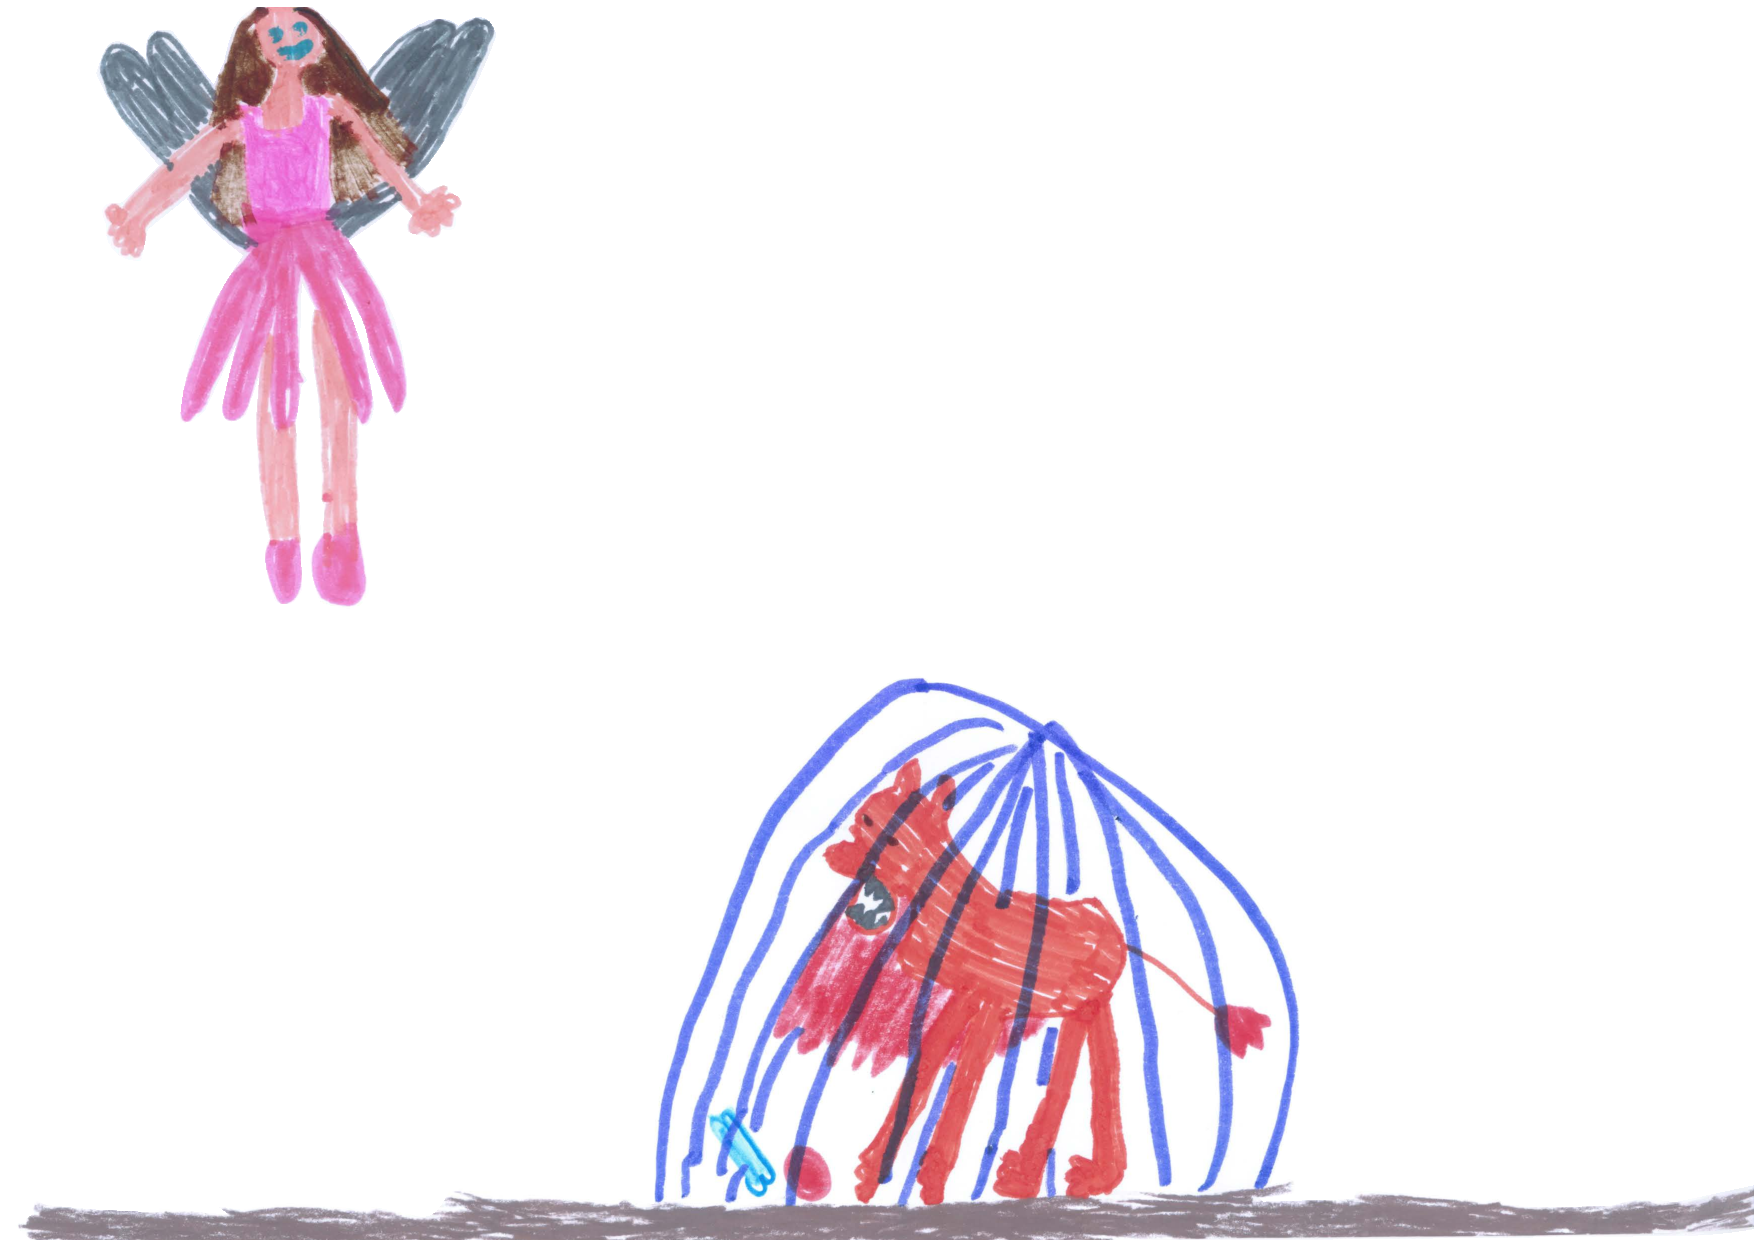
\includegraphics[width=\textwidth,height=.7\textheight]{bilder/loewenalarm.pdf}
\end{figure}
\clearpage
}



Oh je. Jetzt haben die Feen Angst vor dem Löwen bekommen. Das habe ich nicht gewollt, daran hatte ich nicht gedacht beim Malen.  Ich versuche die Feen zu beruhigen, aber es hilft nichts. Immer wieder rufen sie \enquote{Wir haben Angst!}, und
\begin{center}
 {\color{DeepPink}
\large
\itshape
\enquote{LÖ --- WEN --- A --- LARM}}
\end{center}

Dann habe ich eine gute Idee. Ich nehme den blauen Stift und male statt dem Knochen lieber noch einen Käfig um den Löwen. Dicke schwere Gitter und ein Schloss, so gross wie es nur Platz hat. Da kommt der nicht raus, der ist jetzt im Gefängnis einer ganz dicken Burg. Und ich male noch einen Apfel, um zu zeigen, dass das ein Löwe ist, der lieber Äpfel als Feen ist. Gerade will ich das Bild den Feen wieder zeigen, da sehe ich, dass alle Feen wieder zurück in das Bild gekommen sind. Erst eine und dann die anderen hinterher. Genau wie vorhin fliegen sie durch die Luft und verteilen Feenstaub. 

Da bin ich beruhigt, alles ist wieder gut.

Unterdessen sind auch Mama und Papa aufgestanden. Ich erzähle ihnen, was passiert ist, aber Papa, der noch ganz verschlafen ist und sich die Augen reibt, antwortet nur: 

\enquote{Toll mein Schatz, wie du die Feen und den Löwen gemalt hast!} 

Der hat mich wohl gar nicht richtig verstanden. Dass die weg gewesen sind \emph{nachdem} ich sie gemalt habe, hat Papa wohl überhört. Eltern sind manchmal sonderbar, die aufregendsten Dinge im Leben verpassen die immer. \hfill {\color{DeepPink}\decofourleft}

\chapter*{\FontH{\Huge Der grosse Clown kann fliegen}}
\addcontentsline{toc}{chapter}{Der grosse Clown kann fliegen}
\lettrine[lines=3]{\color{red}L}{ouis} und seine Eltern kommen gerade vom Stadtfest zurück. Er hatte im Karussell fahren dürfen und hatte einen Schleckstengel bekommen, der viel grösser ist als seine Hand. Aber sein ganzer Stolz gehört einem Luftballon, der aussieht wie ein Clown. Louis hält den Ballon auf dem Arm.

Als Mama die gerade die Tür aufschliesst kommt die Nachbarin Frau Schweizer.

\enquote{Hach Frau Reichenbach}, ruft sie, \enquote{Sie können es nicht glauben. Meine Neffin liegt im Krankenhaus, ein Unfall, wissen Sie. Die sollte ich dringend besuchen. Ob sie nicht so lange auf Leika aufpassen könnten? Heute Abend bin ich bestimmt zurück.}

Leika ist der Hund von Frau Schweizer. Ein sehr kleiner weisser Hund, der immer kläfft. Louis kann Leika deswegen nicht besonders leiden. Nie kann er mit dem Ball draussen spielen, wenn Leika in der Nähe ist. Der Hund springt dann immer hinter dem Ball her und versuchte den zu beissen, was aber nie klappt, denn sein Maul ist viel zu klein. Frau Schweizer ruft dann immer, dass Leika nur spielen will, womit Louis aber auch nicht geholfen ist. Gegen den Ball treten geht dann nicht mehr ohne Leika weh zu tun.

Aber einen Nachmittag lang kann ja nicht so schlimm sein, denkt sich Louis. Was für ein Irrtum! Schon als allererstes schnappt sich Leika den linken Hausschuh von Louis und rennt damit auf den Balkon.

\enquote{Zieh endlich deine Hausschuhe an!} hört Louis Papa rufen. Pff, als ob er das nicht vorgehabt hätte. Dann schmeisst Leika den Turm um, den Louis und Papa heute Morgen, als Mama noch geschlafen hat, gebaut haben. Louis fängt an mit Leika zu schimpfen, aber Mama ruft aus der Küche, dass das doch nicht so schlimm sein und man den Turm neu bauen könne. Aber Louis will keinen neuen Turm, er will den Turm wieder haben. Er streckt Leika die Zunge raus und schiesst ein Kissen nach ihm.

\enquote{Jetzt reicht es aber!} Papa und Mama sind ärgerlich. Mit Kissen nach kleinen Hunden schiessen ist nicht in Ordnung, finden sie. Als ob dem das weh tun könnte.

\enquote{Und ab in dein Zimmer, Freundchen, bis es Mittag gibt!} heisst es dann auch noch. So eine Ungerechtigkeit, aber egal, Louis will sowieso in sein Zimmer und etwas spielen. Tür zu und erst wieder raus kommen, wenn Frau Schweizer Leika wieder abhgeholt hat, so ist sein Plan.

Aber bevor er die Tür schliessen kann, wird Leika auch in sein Zimmer geschoben. 

\enquote{Du spielst jetzt auch mit Leika}, sagt Mama, \enquote{Wir wollen hier noch im Wohnzimmer putzen und da stört ein Hund sehr. Spiel du mit ihm.}

Das hatte noch gefehlt! Jetzt muss sich Louis um Leika kümmern. Mist! Aber vielleicht genügt es ja, ihn zu ignorieren. Louis sieht sich gerade um, als Leika furchtbar anfängt zu bellen und sich auf den neuen Ballon stürzt. Ausgerechnet! Gerade noch kann Lois ihn wegreissen. Das war knapp. Einen Ball kann Leika nicht zerbeissen, bei einem Ballon ist sich Louis da nicht so sicher.

Er hält den Clown so hoch er kann, aber Leika springt immer wieder an ihm hoch. So ist der Clownsballon zwar erst einmal in Sicherheit, aber lange kann er die Arme nicht so nach oben halten. Dann eben in das Regal mit dem Ballon. Das erste Fach, bei dem es Louis probiert ist schon voll. Kuscheltiere. Das zweite ist zu klein. Beim dritten klappt es. Triumphieren schiebt Louis den Ballon in das Fach.

Leika kläfft dazu die ganze Zeit ununterbrochen. Er will unbedingt an diesen Ballon kommen. So sind Hunde halt, das ist ihre Art zu spielen, aber es nervt eben doch. Plötzlich ist Leika mit einem Sprung, von dem Louis nie gedacht hätte, dass ein so kleiner Hund das kann, auf dem Schreibtisch. Und von dort ist es nicht mehr weit bis zum Regal. 

Louis kann im letzten Moment den Clownsballon aus dem Regal reissen. Dabei fällt er ihm aber durch das offene Fenster.

Selbst Leika verschlägt es den Atem. Louis und Leika sind still und sehen zum offenen Fenster und zu dem Ballon. Louis überlegt gerade, ob es wohl laut poltert, wenn so ein Clownsballon unten auf dem Boden aufschlägt. Und ob er dann wohl in tausend Scherben zerspringen wird, wie neulich Papas Glas, oder ob er nur eine grosse Beule bekommt, wie sein Spielzeugauto.

Aber es passiert etwas ganz anderes, etwas, womit weder Louis noch Leika gerechnet haben. Der Ballon steigt in die Luft!

\enquote{Der grosse Clown kann fliegen!} ruft Louis immer wieder ganz aufgeregt.

Mama und Papa kommen ins Zimmer und wollen wissen, was hier los ist.

\enquote{Hast du nicht aufgepasst?} fragt Papa. \enquote{Na der ist weg.} ergänzt Mama. Beide wollen Louis trösten, aber das ist gar nicht nötig! Der Clown wird schon wissen, warum er weg geflogen ist. Und Louis weiss es auch. Jetzt kann Leika ihm nichts mehr anhaben, jetzt ist er sicher.

Und weil Louis das weiss, macht es ihm auch gar nichts mehr, sich den Rest des nachmittags ein bisschen um den Hund zu kümmern.

 \hfill {\color{red}\decofourleft}

\chapter*{\FontH{\Huge Pinarella}}
\addcontentsline{toc}{chapter}{Pinarella}
\lettrine[lines=2]{\color{red}P}{}inarella war ein Schmetterling. Träge lag sie wie jeden Morgen auf dem Regal im Wohnzimmer der Familie Emil und liess sich die Sonne auf die Flügel scheinen. Sie gähnte so laut das Schmetterlingsdamen eben können und blickte sich gelangweilt im Zimmer um. Pinarella war nämlich kein einfacher Schmetterling, nein, sie bestand aus einem Körper aus Holz und die Flügel waren aus bunter Folie gemacht. Schön sah das zwar aus, aber zum Fliegen taugte so ein Körper nicht. Cornelia, die Tochter der Emils hatte Pinarella gebastelt, als sie so ungefähr in der dritten Klasse gewesen war. Aber das ist jetzt schon viele Jahre her, Cornelia hatte selbst schon zwei Kinder und mit denen war sie gerade zu Besuch bei ihren Eltern. Eigentlich wohnte Pinarella gar nicht auf dem Regal, sondern hing für gewöhnlich an einer Schnur über dem Ofen. Aber das letzte Mal als Cornelia mit den Enkelinnen dagewesen war, ist sie beim Spielen auf dem Boden gelandet und von da hat sie jeman auf das Regal gelegt. Bisher hatte sich noch niemand die Mühe gemacht, sie wieder aufzuhängen, aber das war Pinarella egal. Beide Orte sind genau gleich langweilig, so viel war klar. Deswegen war es auch ganz gleichgültig, wo sie gelagert wurde.


Spielen konnte sie allerdings auch bei den Emils. Besonders Jette, die jüngste Tochter von Cornelia machte das sehr gerne.  Jette war allerdings noch zu jung, um die Schönheit Pinarellas zu verstehen. Sonst würden sie wahrscheinlich nicht gar so garstig und nachlässig mit ihr umgehen. Mal wurde sie an den Flügeln gezogen, die dann umständlich von Frau Emil wieder festgeleimt werden mussten, dann wurde sie unachtsam unter einem Berg Legosteine vergraben. Und einmal wurde sie sogar mit auf die Pergola genommen und dann dort vergessen. Die ganze Nacht fror Pinarella ganz fürchtlerlich.

Jette war allerdings ein liebes Kind, das wusste Pinarella, deswegen nahm sie ihr das alles auch nicht übel. Sie war einfach noch zu jung. So viel wusste Pinarella über die Menschen: wenn sie klein sind, überlegen sie manchmal nicht, was so alles passieren kann, wenn sie dies und jenes machen. Gerade gestern ist Jette in alleine in ihr Stühlchen geklettert und dabei sehr unsanft abgestürzt. Das war ein Weinen! Und Jette hatte sich selbst bestimmt nicht mit Absicht weh getan, hatte Pinarella überlegt und so ging es wohl auch mit ihr, wenn Jette ihr mal wieder einen Fühler abgebissen hatte.

Auf dem Regal war Pinarella jetzt zwar sicher vor Jette, aber eben auch alleine. Jette war viel zu klein, um sie so weit hoch zu kommen. Lieber wieder einen Flügel verlieren, dachte Pinarella, als den ganzen Tag hier zu liegen. 

\enquote{Schade} seufzte Pinarella, \enquote{wirklich schade, dass ich kein richtiger Schmetterling bin. Es ist ja schon lustig, mit Jette zu spielen, aber die ist einfach so selten zu Besuch. In der Zwischenzeit ist es doch immer sehr langweilig. Da wäre es ja doch viel lustiger, wenn ich hinaus fliegen könnte in die Welt, um mit anderen Schmetterlingen zu spielen.} 

An diesem Morgen war Jette mal wieder sehr früh munter geworden. Cornelia, die Jette selbstverständlich nur \enquote{Mama}  nannte und sie waren im Wohnzimmer und Cornelia war wieder eingeschlafen. Pinarella hatte das gar nicht gemerkt. Jette sass auf dem Boden und versuchte vergeblich ihrem Püppchen die Hosen anzuziehen. Wenn man erst zwei Jahre alt ist, klappt so etwas manchmal noch nicht so gut und ausserdem waren es sowieso Hosen für eine viel kleinere Puppe. Die Sache klemmte und damit auch die Lust von Jette, weiter mit der Puppe zu spielen. Gerade als sie sich umsah, um zu sehen, womit man als nächstes so spielen könnte, hörte sie die Klage von Pinarella. 

\enquote{Was ist denn mit dir los?} fragte Jette. Pinarella war verwirrt. Schon oft hatte sie versucht mit Menschen zu reden, aber so laut sie auch geschrieen hatte, nie hat sie jemand gehört.

\enquote{Kannst Du mich verstehen?} fragte sie daher ganz ungläubig. 

Jette nickte bloss. 

\enquote{Mir ist langweilig.} sagte Pinarella, niemand spielt mit mir, meine Flügel sind schon voller Staub.

\enquote{Dann komm doch hier zu mir geflogen!} schlug Jette vor, die den Unterschied zwischen einem echten Schmetterling und einem gebastelten noch nicht so genau kannte. Und obwohl Jette das gar nicht so genau interessierte, erklärte Pinarella ihr den Unterschied. Ihr war das nämlich wichtig. Jette verstand nicht alles, aber eines war klar: Pinarella wollte auch gerne fliegen können, um mit anderen Schmetterlingen spielen zu können. Das verstand Jette sogar gut, sie spielte ja auch am liebsten mit anderen Kindern.

\enquote{Dann helfe ich Dir!} beschloss Jette, hatte aber noch keine Ahnung, wie. Aber das ist normal bei Zweijährigen. Die beschliessen immer Sachen, von denen sie noch nicht wissen, wie man das dann genau macht. Zuerst musst Pinarella mal von dem Regal herunter, das war offensichtlich. Das Regal war schon sehr hoch, sogar noch höher als Papa gross ist, schätzte Jette. Der konnte einen aber hoch nehmen, wenn man die Arme in die Luft streckt, Regale machen so etwas wohl aber nicht. Jette hatte bereits ein bisschen Lebenserfahrung. Und die sagte ihr auch, dass man wohl etwas zu Hilfe nehmen musste.

Die beide sahen sich im Zimmer um, was wohl genau diese Hilfe sein könne. Jette hatte plötzlich eine Idee. Wenn sie mit dem Wasserhahn vom Waschbecken spielen wollte, schob sie sich immer das Schemelchen hin und stieg darauf. Für das Waschbecken war sie nämlich auch noch zu klein.  Aber das Schemlechen war natürlich im Badezimmer und wenn man dort hin wollte, würde Mama bestimmt munter werden. Pinarella und Jette mussten seufzen. Beinahe gleichzeitig sahen sich die beiden an, dann zum Stuhl, dann wieder sich. So leise wie eine Zweijährige eben kann, lief Jette zu dem Stuhl und schob ihn so vorsichtig wie möglich in Richtung Regal.

\enquote{Mach keinen Quatsch!} Mama war von dem Quitschen munter geworden, drehte sich aber zum Glück nochmals auf die Seite und schlief weiter. Jette und Pinarella hatten den Atem angehalten, den Jette mit einem lauten {\it Pffff.} jetzt wieder raus liess. Das war knapp. Wenn Mama gemerkt hätte, was Jette vor hat, wäre sie bestimmt dagegen gewesen. Ganz leise kletterte Jette jetzt auf den Stuhl. Noch immer reichte sie nicht bis oben hin. Zum Glück sah Jette sofort dendem Rückenkratzer vom Opa, den konnte sie nehmen und tatsächlich! Es klappte! Jette kam gerade so bis an das obere Ende des Regals, konnte Pinarella an einem Fühler erwischen und zog sie vom Regal herunter.

Mit einem leisen {\it Plopp} landete Pinarella auf der Couch, aber zum Glück weit genug von Mama entfernt. Jette kletterte vom Stuhl herunter, was gar nicht so einfach war, nahm Pinarella, öffnete das Fenster und mit einem lauten 

\enquote{Jippie, flieg Pinarella!} war Jette den Holzschmetterling aus dem Fenster.

Natürlich konnte Pinarella nicht fliegen. Sie stürzte jäh ab und raste in Richtung Boden. 

\enquote{Da wird bestimmt noch mehr kaputt gehen, als nur ein Fühler.} dachte Pinarella. Gerade in dem Moment ging die Sonne hinter den Bergen auf. Und genau als Pinarella in der Luft war, traf sie der allererste Sonnenstrahl des Tages. Pinarella konnte ihn auf ihren Flügeln spüren und instinktiv zuckte sie zusammen und da geschah es. Ihre Flügel bewegten sich! Erst langsam, dann immer schneller und noch bevor Pinarella auf dem Boden aufschlagen konnte, flog sie. Aus der Spielzeugpinarella war ein richtiger Schmetterling geworden. Höher und immer höher flog sie, fast so hoch wie das Haus und wieder runter zu dem Blumen auf der Wiese und einfach immer weiter. Jette jubelte vor Freude und Mama, die von ihrem geschrei munter geworden war, guckte ganz verschlafen, was da los ist.

\enquote{Und nur wegen einem Schmetterling machst du so einen Lärm, dass du mich wecken musst?} Jette musste lächeln, Mama hatte nicht gemerkt, dass sie selbst den Schmetterling gebastelt hatte, der da geflogen war. \hfill {\color{red}\decofourleft}
\begin{figure}[ht]
\centering
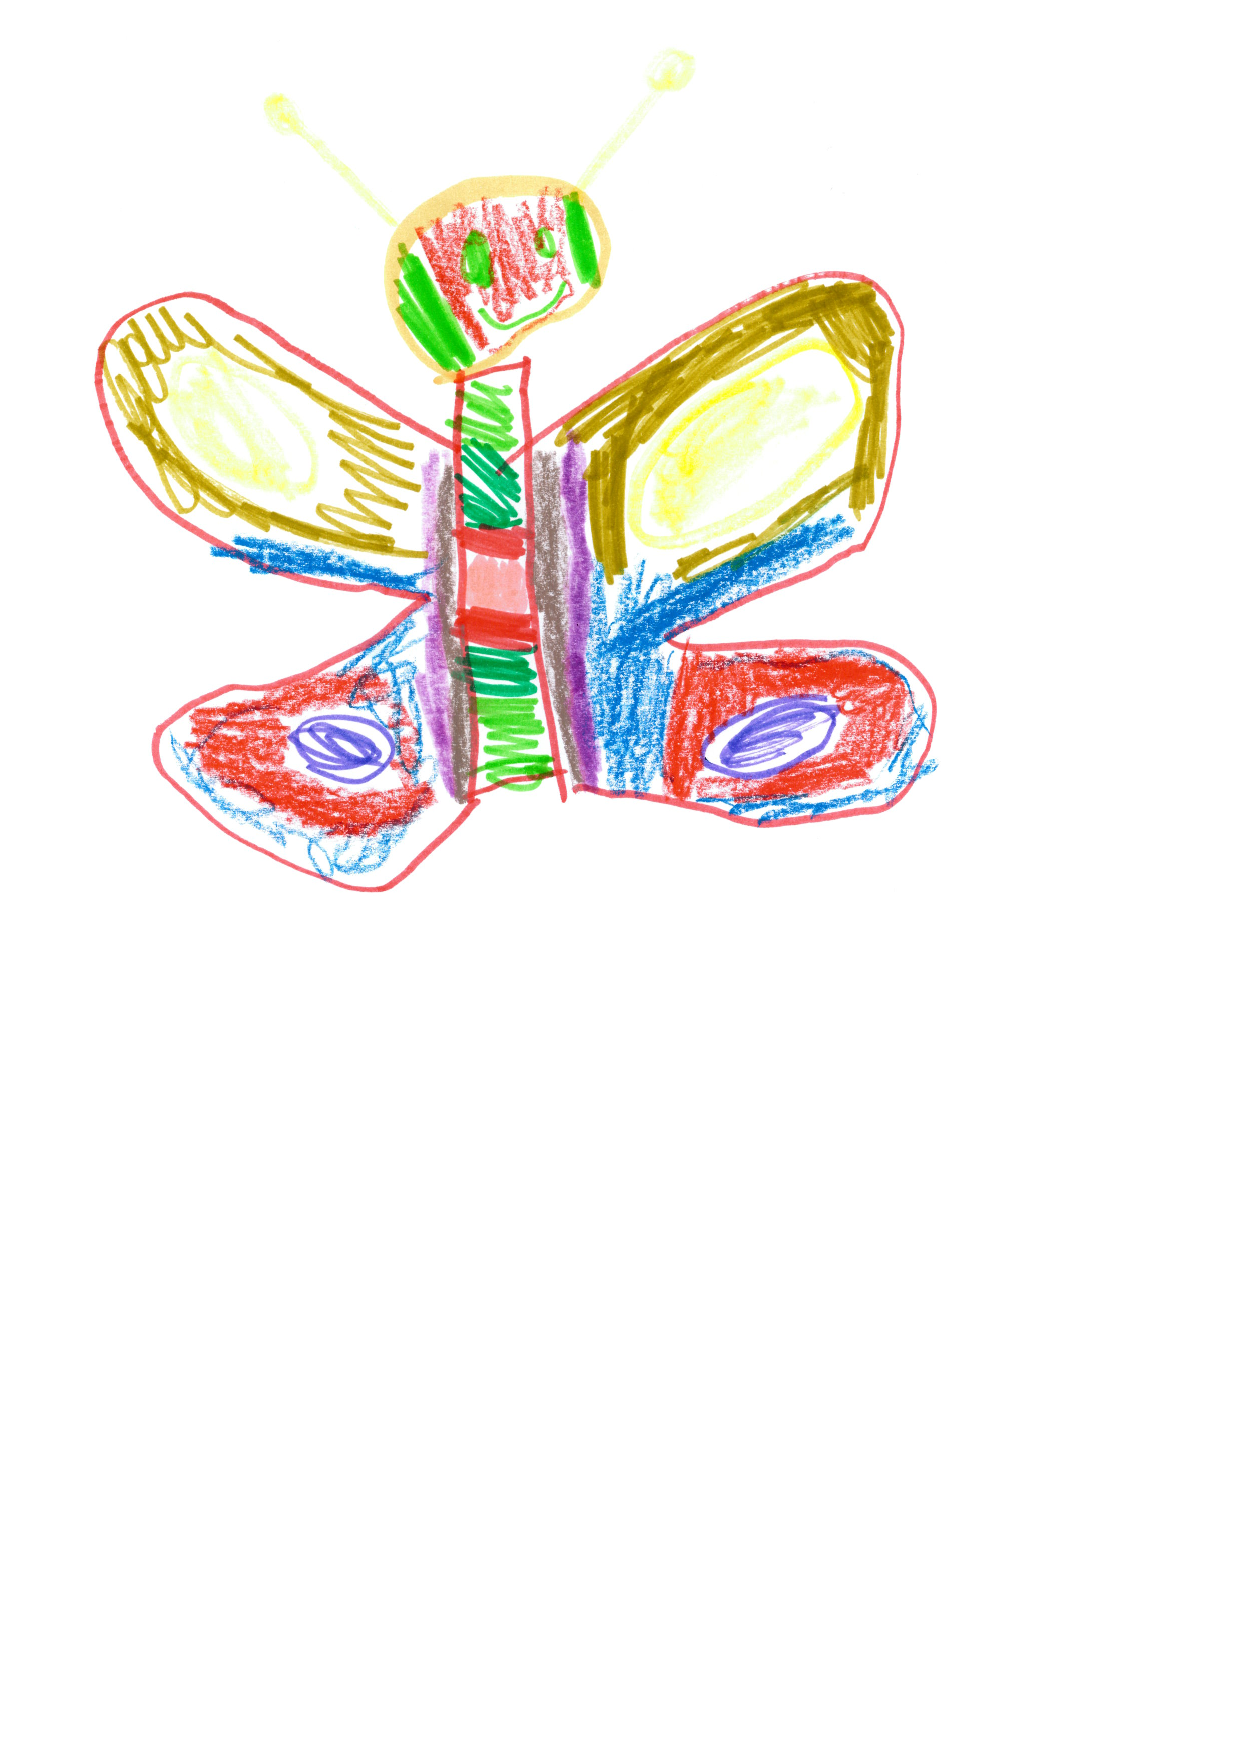
\includegraphics[scale=0.5]{pinarella.pdf}
\end{figure}

\chapter*{\FontH{\Huge Milch und Eis}}
\addcontentsline{toc}{chapter}{Milch und Eis}
\lettrine[lines=3]{\color{red}H}{och} im Norden, wo es immer Winter ist, liegt das Reich der Schneekönigin. Sie lebt in einem Palast ganz aus Eis und sogar die Möbel bestehen aus Eis. Wenn im Palast jemand durstig ist, bricht man einfach ein Stück Eis von der Wand ab und wartet bis es im Munde geschmolzen ist.

Von einem Händler aus dem fernen Süden erfuhr die Schneekönigin eines Tages, dass es Tiere namens Kühe gibt, die Euter unter ihrem Bauch tragen, aus denen, wenn man es nur richtig anstellt, eine weisse Flüssigkeit gemolken werden kann, die Milch genannt wird. Das fand die Schneekönigin aufregend und wollte unbedingt auch einmal ein Glas dieser Milch probieren.

Also schickte sie einen Diener los, der eine solche Kuh in ihr Reich bringen möge. Nach einer langen beschwerlichen Reise konnte der Diener eine Kuh beschaffen. Aber da diese so hoch im Norden nirgends Gras finden konnte und es ihr überhaupt viel zu kalt war, weigerte sie sich Milch zu geben. Ausserdem war sich niemand im Palast so ganz sicher, was es mit diesem Melken auf sich hatte. Schon nach einer Woche gab die Schneekönigin auf und liess die Kuh zurück in den warmen Süden bringen.

Der Diener, der dazu beauftragt worden war, erhielt auch gleich noch die Anweisung, ein Glas Milch mitzubringen. Wenn die Schneekönigin schon keine eigene Kuh halten konnte, dann wollte sie doch trotzdem weiter Milch probieren. Als der Diener zurück kam und die Königin endlich einen grossen Schluck nehmen wollte, wurde ihr ganz übel, denn die Milch war auf der langen Reise sauer geworden. Damit hatte niemand gerechnet. 

Die weisesten Männer und Frauen des Landes wurden zusammengerufen und sollten Ratschläge erteilen, wie die Milch denn die Reise überstehen könne. Diese wiegten den Kopf hin und her und gaben so alle möglichen Tipps, aber es war klar, dass eigentlich niemand eine Ahnung hatte. Die Tochter einer Dienerin wusste dann aber doch etwas Überzeugendes, denn die guckte immer die Sendung mit der Maus. Milch, so erklärte sie, werde weniger schnell sauer, wenn man sie nur richtig kühle; im Süden stellen die Menschen sie in Kühlschränke.

Etwas zu kühlen war nun die Spezialität der Königin. Sie schuf einen grossen Klotz Eis, der in der Mitte einen Hohlraum hatte. Der Eisklotz war so gross, dass wenn er in den Süden und zurück gebracht wurde, zwar beginnen würde zu schmelzen, aber eben nicht ganz. So blieb die Milch die ganze Zeit von Eis umschlosen und damit kühl. So wurde der Diener wieder auf die Reise geschickt und er konnte einen Bauern finden, der ihm ein Glas voll Milch in den Hohlraum in dem Eisklotz schütten konnte.

Als der Diener mit dem Rest des Eisklotzes wieder bei der Schneekönigin ankam, war aber auch die Milch in seinem Inneren gefroren. Und im Palast war es so kalt, dass sie unmöglich wieder auftauen könne. Da ja alles aus Eis bestand, waren Wärme und Feuer streng verboten. Enttäuscht liess sich die Schneekönigin auf ihren Thron plumpsen. Der Koch der Königin, ein Italiener namens Gelato war aber ein äusserst raffinierter Vertreter seines Berufes. Er schnitt die gefrorene Milch erst so klein er konnte. Dann zerdrückte er die kleinen Stücke mit der Gabel, um sie dann nochmals kräftig zu rühren, bis eine cremige, kalte Masse entstanden war. In Erinnerung an die saure Milch fügte er zur Sicherheit auch gleich noch etwas Zucker hinzu.

Und das Resultat schmeckte wunderbar. Die Schneekönigin war begeistert und alle die probieren durften auch! Noch viel mehr Milch musste in ihren Palast gebracht und zerkleinert und verrührt werden. Schon bald fügte der Koch Gelato noch andere Geschmacksrichtungen seinem Rezept hinzu. Vanille und Schokolade, Erdbeeren, Nüsse und Pistazien und was sonst so vom Händler geliefert werden konnte.

Sehr schnell verbreitete sich die Idee Milch zu frieren und zu rühren über die ganze Welt und noch heute nennt man diese feine und kalte Creme in Italien {\it gelto} zu Ehren ihres Erfinders.  \hfill {\color{red}\decofourleft}

\chapter*{{\FontH{\Huge Nina und die rosa Delphine}}\\\small \color{red} Oma Carola gewidmet}
\addcontentsline{toc}{chapter}{Nina und die rosa Delphine}
\lettrine[lines=3]{\color{red}H}{eute} war Oma Lena zu Besuch. Nina hatte sich schon lange auf sie gefreut. Oma Lena wohnte leider weit weg, in einem anderen Land, und deswegen konnten sich die beiden nicht so oft sehen. Aber jetzt war es wieder so weit. 

Es war schon spät geworden, Geschenke mussten ja noch ausgepackt werden und dann Abendessen. Nina fand, dass Erwachsene immer viel zu viel Zeit mit Essen vergeuden. Anstatt stundenlang am Tisch zu sitzen, könnte man die Zeit doch viel besser nutzen. Sie würde das später, wenn sie gross sein würde, anders machen, so viel war klar.

\enquote{Also gut}, rief der Papa aus der Küche, \enquote{Oma darf dir noch eine Geschichte vorlesen. Aber nicht mehr so lange. Eine Viertelstunde, höchstens! Morgen ist wieder Kindergarten und dann musst du fit sein, Nina.}

Nina seufzte. Als ob das jetzt wichtig wäre, dass sie morgen früh aufstehen muss. 

\enquote{Ist doch mir egal.}, brummte sie und streckte die Zunge raus, aber so, dass Papa das nicht sehen konnte. Oma Lena hatte ein Buch mitgebracht, das war ihr Geschenk gewesen. Eine Geschichte von rosafarbenen Delphinen. Mama meinte, dass es die wirklich gäbe. Weit weg in einem Fluss namens Amazonas, der mitten durch einen Urwald fliesst. Nochmals schnell auf der Karte nachsehen, wo der eigentlich liegt.

Nach dem Zähneputzen konnte Nina endlich ins Bett springen und auf Oma warten. Nina überlegte, ob Mama ihr manchmal extra lange die Zähne putzte, um sie zu ärgern. Man könnte schon manchmal den Eindruck haben. Kater Fritz war auch gekommen, das war so seine Gewohnheit. Er sprang auf die Decke von Nina und wollte wohl auch zuhören. Fritz und Nina waren gute Freunde, obwohl er manchmal alleine mit Ninas Sachen spielte und die dann weg waren. Manchmal dauerte es Tage, bis die Sachen in irgendeiner Ecke wieder auftauchten. 

Oma setzte sich auf die Bettkante, klappte das Buch auf und blätterte ein bisschen zwischen den Seiten.

\enquote{Bis hierhin lese ich Dir heute vor, den Rest dann morgen. Einverstanden?} Oma tippte dazu auf eine Seite mit dem Bild eines Delphins. 

\enquote{Naaa gut.}, antwortete Nina. Was sollte sie auch machen? Erst einmal anfangen, der Rest würde sich später von alleine finden.

\vspace{10pt}
 \centerline{\Huge \Dolphin[red]}
\vspace{10pt}

Der Urwald ist für gewöhnlich ein ziemlich lauter Ort. Es scheint, dass jedes Tier noch lauter sein wollte als die anderen. An einem Nebenarm des Amazonas war es diesmal besonders laut, denn es wurde ein grosses Fest gefeiert. Die Regenzeit, die grosse Teile des Urwaldes unter Wasser gesetzt hatte, war so langsam vorbei. Nur gelegentlich gab es noch einen Sturm. 

Rosa hatte heute Geburtstag. Den Fünften. Rosa war ein Delphinkind, das in eben jendem Nebenfluss des Amazonas lebte. Die Bäume am Rande des Flusses waren festlich geschmückt. Papageien hatten bunte Federn aufgehängt. Zusammen mit den Schmetterlinge, die überall durch die Luft schwirrten, war das war ein herrlicher Anblick. Ein Ameisenbär steckte seinen Rüssel ins Wasser und machte Blasen, dass es nur so spritzte. Selbst das Faultier drehte seinen Kopf, um zu sehen, was da los ist. Und das musste was bedeuten, Rosa konnte sich nicht erinnern, überhaupt schon einmal gesehen zu haben, dass sich das Faultier bewegt hatte.

Rosas Geburtstag war ein grosses Ereignis. Der fünfte Geburtstag ist nämlich bei Delphinen etwas ganz besonderes. Dann dürfen sie zum ersten Mal alleine aus dem Nebenfluss in den riesigen Amazonas schwimmen. Es ist Tradition, dass sie dann mindestens einen Tag alleine im Amazonas sind. Wer das schafft, ist erwachsen. Ausser Mama und Papa müssen die anderen Delphine dann \enquote{Sie} zu einem sagen. Weil Delphine nicht so alt werden wie wir Menschen, sind sie schon mit fünf Jahren keine Kinder mehr. Aber ganz ausgewachsen sind sie dann auch noch nicht.

Der erste eigene Ausflug ist immer etwas Besonderes. Aufpassen, heisst es dann, denn es lauern viele Gefahren. Am gefährlichsten sind die Alligatoren. Wenn man da als kleiner Delphin nicht aufpasst, macht es Schnapp und weg ist man. Aber fünfjährige Delphine sind so gute Schwimmer, dass das eigentlich nie passiert. Auch vor Zitteraalen muss man sich hüten. Wenn man die berührt, versetzen sie einem einen Stromschlag, der sehr wehtun kann. Onkel Konrad war das mal passiert, tagelang hatte er gejammert.

Rosa hatte natürlich ihre vier besten Freunde eingeladen. Es gab Fischkuchen, so wie ihn nur die Oma backen konnte. Rosas Freunde waren auch schon alle fünf, sie war die letzte. Sie hatten sich vorgenommen, den ersten Ausflug in den Amazonas gemeinsam zu machen. Anders hätten das ihre Eltern auch nicht erlaubt. Und jetzt zum Ende der Regenzeit war der beste Augenblick. Alle waren natürlich aufgeregt, vor allem aber die Eltern. Bevor es los ging, führten die Affen noch ihr traditionelles Spiel auf. Dabei klauen sie sich gegenseitig eine Kokusnuss und die anderen müssen ehrausbekommen, wer es war. Rosa und ihre Freunde durften heute auch mitspielen.

Nachdem der letzte Fischkuchen verputzt war und alle Glückwünsche entgegen genommen worden waren, konnte es endlich los gehen Rosas Mama hatte eine Träne im Auge, als sie ihr hinterher gewinkt hatte, aber unter Wasser hat das natürlich niemand bemerkt. Unterwassertränen sieht man nicht, lautet ja auch ein Delphinsprichwort. Rosa wusste es trotzdem. Jetzt war es aber an der Zeit, mit Fünf muss man das versuchen! Die erste Angst war schnell überwunden. Alle fünf Delphine mussten eingestehen, so ein kleines Kribbeln im Bauch zu haben, als sie ausser Sichtweite ihrer Eltern waren. Dass das auch ein bisschen Angst sein könnte, wollte niemand von ihnen glauben.

\enquote{Ach was, wir haben einfach nur zu viel Fischkuchen gegessen.}, hiess es dann, und weiter ging es. Plötzlich war ein riesiger Schatten zu sehen. Rosa musste kurz aufschreien, aber es konnte schnell Entwarnung gegeben werden. Ein Arapaima schwamm träge durch das trübe Wasser. Arapaimas sind sehr grosse Fische. Im Amazonas sind nur Alligatoren noch grösser. Er brummte einen Gruss, Höflichkeit ist ausgesprochen wichtig im Amazonas, das gilt auch für alte, knorzige Arapaimas.

\enquote{Ein Sturm zieht auf. Schwimmt zwischen die Mangrovenwurzeln, rate ich euch!}, meinte er ohne anzuhalten. 

Den fünf Freunden war das natürlich egal. Ein Sturm mag ärgerlich sein, wenn man an Land lebt, aber als Delphin im Wasser kann ja nichts passieren. Ob es oben noch regnet, ist ja dann egal. Und so tollten sie herum. Sie hatten sich schnell an ihre neue Freiheit gewöhnt. Niemand der da war und sagte, passt auf, da kommt ein Holzstamm geschwommen. Oder: nicht so den Schlamm aufwühlen! Sachen, die Erwachsene eben so zu Kindern sagen. Mit ihren Schwänzen wirbelten sie heute gemeinsam so viel Schlamm auf, dass das aussah wie ein Vulkanausbruch, wenn man vom Ufer zusah.

Dann jagten sie zusammen Fische, sogar die gefährlichen Piranhas. Der Trick war, sie von der Seite zu erwischen, dann konnten sie einen nicht beissen. Weiter ging's mit Versteckspielen, das spielen wohl alle Tierkinder auf der Welt gerne.

Dass sich der Himmel immer mehr verdunkelt hatte, bemerkten sie gar nicht richtig. Der Wind frischte auf und wurde schnell immer stärker. Aus dem sanften Amazonas wurde eine wilde Welt aus Bergen und Tälern von Wasser. Der Urwald heisst in der Gegend hier nicht umsonst Regenwald. Erst spielten die fünf mit den Wellen, aber schnell wurden sie von ihnen mitgerissen.

Die gute Laune kippte. Jetzt schämte sich auch keiner der Fünf mehr Angst zu haben. Weder Rosa noch die anderen wussten sich zu helfen. Der Amazonas riss sie einfach mit, da half keine Anstrengung. Ach, hätten sie nur auf den alten Arapaima gehört! Zwischen den Wurzeln wären sie sicher gewesen. Aber jetzt war das zu spät, jetzt mussten sie gegen das Wasser kämpfen. Ganze Bäume waren ausgrissen und schwammen mit dem Amazonas mit. Da durfte man sich nicht in den Ästen verheddern und musste immer ausweichen. Der Sturm dauerte viele Stunden. Alle waren damit beschäftigt gewesen, aufzupassen, nicht von den Wellen gegen irgendetwas geschleudert zu werden und nahe zusammen zu bleiben. Keiner von ihnen hatte bemerkt, wo sie eigentlich hingespült wurden.

Als der Sturm sich soweit gelegt hatte, dass man sich wieder verstehen konnte, sagte Rosa:

\enquote{Na prima.} Und dabei hatte sie eine kleine Träne im Auge. \enquote{Was für eine Geburtstagsfeier!}

Die Fünf sahen sich um, nichts, aber auch wirklich gar nichts war zu sehen. Nur Wasser, soweit das Auge reichte. Rosa versuchte es mit einem Sprung aus dem Wasser, um besser sehen zu können. Auch nichts. Kein Baum, kein Strauch, kein Vogel.

\enquote{Was ist mit dem Urwald passiert?}, fragten sie sich gegenseitig. \enquote{Ist der vollständig überschwemmt? Gibt es keine Bäume mehr, ist jetzt alles Amazonas? Und warum schmeckt das Wasser hier so furchtbar?} 

Tatsächlich schmeckte das Wasser sehr salzig. Viel Zeit zum Grübeln blieb ihnen aber nicht. Noch bevor sie wirklich verzweifelt sein konnten, durchschnitt ein graues Dreieck die Wellen und kam direkt auf sie zu. Erst bemerkte es niemand, aber als es immer schneller wurde, rief Rosa:

\enquote{Achtung, da kommt etwas!} Das graue Dreieck war die Rückenflosse eines grossen Fisches. Als er sein riesiges Maul aufriss, konnten sie drei Reihen sehr scharfer und spitzer Zähne sehen. Ein Hai? Von denen hatten die Fünf schon gehört. Die lebten doch im Meer? Waren sie etwa im Meer gelandet? Sie schwammen um ihr Leben. Zuerst schnell in alle Richtungen wegschwimmen, um das Ungeheuer zu verwirren, dann wieder sammeln, um sich nicht zu verlieren. So hatten sie es zu Hause gelernt und geübt.

Aber der Hai griff immer wieder an. Er kam auf die Fünf zugeschossen und riss sein furchtbares Maul auf. Jedes Mal verfehlte er sie, aber immer etwas knapper. Viel Kraft, ihm immer wieder auszuweichen, hatten sie nicht mehr. Alle hatten furchtbare Angst. Wieder blitzen die Zähne des Hais auf. Er raste auf Rosa zu. Die konnte sich vor Schreck und Erschöpfung nicht mehr bewegen. Wie versteinert blieb sie stehen. 

Plötzlich zeigte sich etwas im Wasser, dass für die Delphine aussah wie eine riesige Kokosnuss. Er kam mit grossem Schwung und stiess den Hai mit voller Wucht in die Seite, so stark, dass der sich im Wasser überschlagen musste.  Aber er hatte Rosa noch an der Schwanzflosse erwischt. Nicht sehr schlimm, aber sie blutete ein bisschen und es tat furchtbar weh. Der grosse Berg entpuppte sich als eine grosse Schildkröte. 

Der Hai drehte ab und schwamm noch ein paar Mal hin und her. Die Seite tat ihm doch gehörig weh, weswegen er sich etwas zurückzog. Noch so einen Schlag von dieser Schildkröte hätte er nicht verkraftet. Er schwamm etwas zur Seite, sicher ist sicher, aber gerade so, dass er die Delphine noch sehen konnte. Schildkröte hin oder her, die Delphine sahen schon lecker aus.

Die Schildkröte stellte sich den Delphinen als Florian vor. Und obwohl Florian, wie alle Schildkröten, sonst eher der gemütliche Typ war, hielt er sich nicht lange mit Vorstellen auf und meinte: 

\enquote{Der Hai ist noch in der Nähe. Kommt mit mir mit, schnell! Alle nochmals gut Luft holen und los!}

Alle atmeten tief ein und tauchten hinter Fridolin her. Tiefer und immer tiefer tauchte der. So tief, wie der Amazonas an keiner Stelle war, so tief, wie das nur im Meer geht. Delphine und Schildkröten können ja nicht wie Fische unter Wasser atmen, sondern müssen immer an die Wasseroberfläche kommen. Der Hai folgte ihnen in gebührendem Abstand. Die fünf Freunde hatten das Gefühl, es nie wieder bis nach oben zu schaffen, so lange hatten sie jetzt schon die Luft angehalten. Selbst Fridolin, amtierender Lateinamerikameister im Luftanhalten, hatte einen roten Kopf bekommen. 

Sie schwammen immer weiter und weiter und tauchten an einer Felswand entlang. Die war eigentlich wunderschön, denn überall glitzerten und glänzten die schönsten Kristalle. Endlich flüsterte Fridolin:

\enquote{Dort hinter den langen Algen ist der Eingang zu einer Höhle. Dort müsst ihr hinein schwimmen. Da könnt ihr dann auch wieder atmen. Ich lenke solange den Hai ab.}

Fridolin raste auf den Hai los. Der war erst ganz erschrocken, öffnete dann aber seinen riesigen Mund und zeigte seine gefährlichen Zähne. Aber Fridolin liess sich nicht beirren. Schnurstracks sauste er in die Richtung des Hais. Als er ganz dicht an ihm dran war, biss der Hai zu. Im letzten Moment zog Fridolin die Beine und den Kopf ein, so dass nur noch sein Panzer zu sehen war. Der schützte ihn. So ein Haibiss macht einer Schildkröte nichts aus, jedenfalls, wenn es bei einem Biss bleibt. Deswegen schwamm Fridolin schnell hinter den Delphinen her, solange sich der Hai um seine Zahnschmerzen kümmern musste.

Die fünf Freunde hatten den Eingang zur Höhle längst gefunden. Davon hatte der Hai natürlich nichts mitbekommen. Dort schwammen sie hinein und konnten auch wieder Luft holen. Eine Höhle unter dem Meer, in der es Luft gab! Von weit weg drang etwas Licht herein. Der Hai hatte zwar bemerkt, dass sich alle hier irgendwo versteckt haben mussten, er konnte aber nicht erkennen, wo. Also wartete er und legte sich auf die Lauer.

Die fünf Freunde mussten hächeln. Keiner von ihnen hatte schon jemals so lange die Luft angehalten. Es war eigenartig still hier in der Höhle. Wenn man im Urwald wohnt, hat man nämlich noch nie einen so ruhigen Augenblick erlebt. Die Stille wurde aber unterbrochen als Fridolin mit einem lauten: 

\enquote{Paaaahhhhhh.} angetaucht kam und auch erst einmal tief Luft holen musste.

\enquote{Ist jemand verletzt?}, fragte Fridolin, nachdem er sich erholt hatte. Er selbst war unverletzt, nur ein grosser Kratzer zierte jetzt seinen Panzer. Den würde er jetzt für immer als Erinnerung behalten. Nur Rosa hatte eine schwere Schramme abbekommen. Den anderen ging es gut, aber sie alle waren sehr erschöpft.

\enquote{Das heilt wieder.}, meinte Fridolin, nachdem er sich die Wunde angesehen hatte. \enquote{Ihr bleibt hier und ich hole uns erst einmal ein paar Fische.}

Die fünf Freunde schlangen die Fische herunter. Langsam kehrten auch ihre Kräfte zurück. Während sie assen, erklärte Fridolin, dass er eigentlich ursprünglich gar nicht aus der Gegend sei, sondern von den Galapagos-Inseln stamme, die noch weiter im Meer draussen liegen. Aber bei einem Ausflug hätte er diese Höhle hier gefunden und die habe ihm so gut gefallen, dass er an freien Wochenenden oft Ausflüge hierher unternähme. Datsche nannte er die Höhle und musste lachen, aber die Fünf waren nur verwirrt. 

Dann mussten sie ihrerseits Fridolin ganz genau erklären, was passiert war. Der wiegte den Kopf hin und her und meinte, dass der Sturm sie wohl ins offene Meer getragen habe. Sie sollten sich keine Sorgen machen, es würde alles wieder gut werden. Abwarten, bis der Sturm vorbei ist und der Hai die Suche aufgegeben hätte. Dann würde er ihnen den Weg zurück zeigen.

Aber das war leichter gesagt als getan. Rosa Flosse blutete immer noch, sie konnte unmöglich nochmals so lange tauchen. Und weil ihr Kopf aus dem Wasser guckte, konnte man ausnahmsweise sehen, wie einem Delphin grosse Tränen aus den Augen kamen.

\begin{figure}[h]
\centering
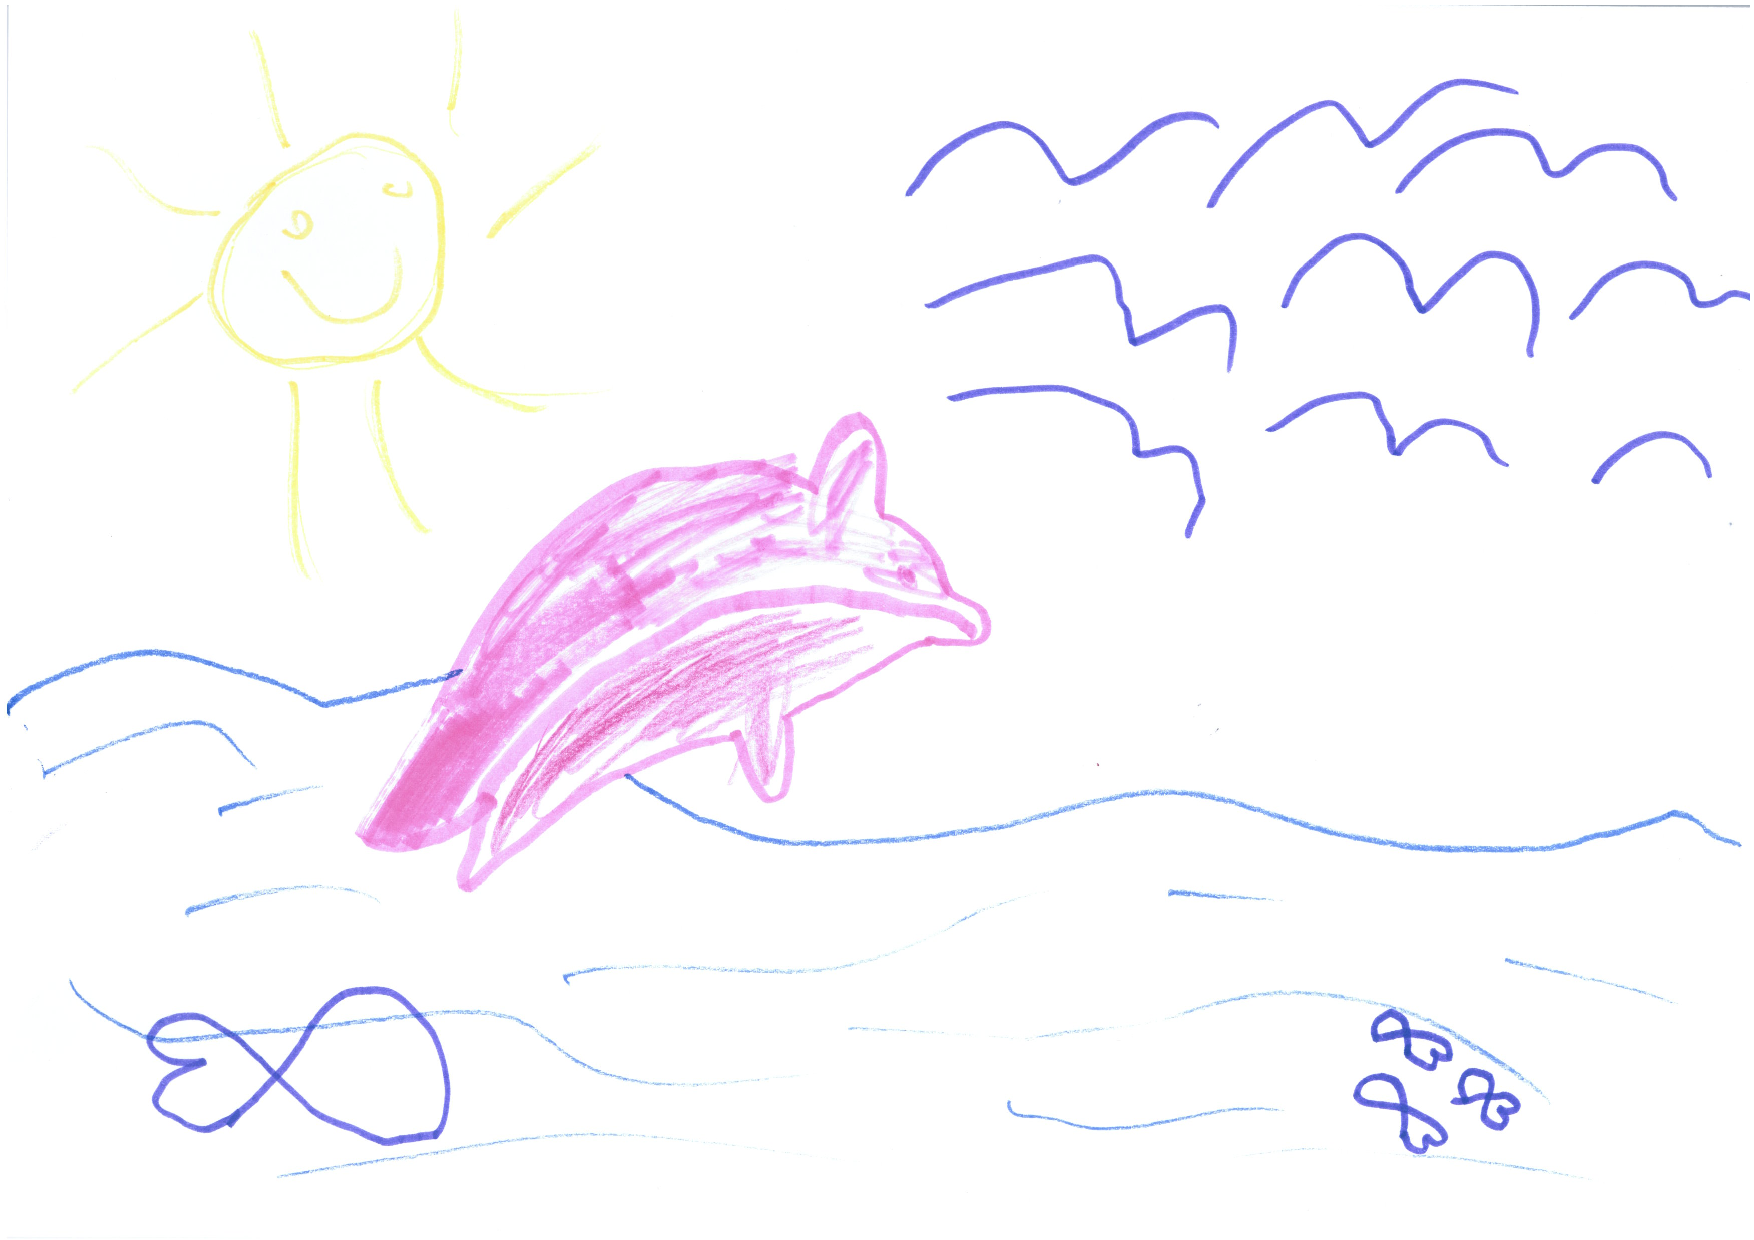
\includegraphics[width=.7\textwidth]{bilder/oma1.pdf}
\end{figure}

\vspace{10pt}
 \centerline{\Huge \Dolphin[red]}
\vspace{10pt}

Sie waren auf der Seite mit dem Delphinbild angekommen. Es war Rosa, wie sie gerade aus dem Wasser sprang. Eine schöne Zeichnung, dachte Nina. Oma klappte das Buch zu und gab Nina einen Kuss auf die Stirn.

\enquote{Schlaf gut, mein Engel.}, sagte sie \enquote{Und morgen, gleich wenn Du aus dem Kindergarten zurück bist, lese ich Dir den Rest der Geschichte vor.} Selbstverständlich protestierte Nina. Wie kann man nur so gemein sein und aufhören, wenn es am spannendsten ist! Das war jetzt schon das zweite Mal an diesem Abend, dass sie sich vornehmen musste, es später, wenn sie selbst gross sein würde, besser zu machen. Aber noch bevor sie das Oma erklären konnte, musste sie so fest gähnen, dass sie beschloss, auf lauten Protest zu verzichten. Kater Fritz wurde noch aus dem Zimmer gescheucht, die Tür blieb einen Spalt offen und Nina schlief sofort ein.

Am nächsten Morgen konnte es Nina kaum abwarten, wie die Geschichte wohl weiterging. Die arme Rosa! Wie sie wohl wieder aus der Höhle kommen würde? Nina kontrollierte nochmals, ob das Buch auch so lag, dass sie gleich weiter lesen konnten, wenn sie zurück vom Kindergarten kam. Sie hatte so lange bei Mama gequängelt, bis diese versprochen hatte, dass es das Mittagessen erst gibt, wenn die Geschichte zu Ende erzählt war.

Endlich war der Kindergarten vorbei. Ohne wie sonst auf ihre Freundinnen zu warten, rannte Nina nach Hause. Oma sass schon lachend auf der Couch und meinte, Nina solle das Buch holen, es könne gleich los gehen.

Aber das Buch war nicht mehr da! Weg!

\enquote{Maaaaamaaaa, Maaaaaaaaamaaaaa! Wo hast du das Delphin-Buch hingelegt?} Nina war ausser sich. Mama kam die Treppe hinauf.

\enquote{Ich hab' dein Buch nicht, Schatz. Wo hast du es denn hingelegt?} Auf so eine Frage antwortete Nina gar nicht erst. Als ob sie da nicht als allererstes gesucht hätte. Verzweifelt riss sie alle Bücher aus dem Büchergestell, aber das Delphin-Buch war nicht dabei.

Nina verzog sich in ihr Bett und schmollte. Mama versuchte zu trösten und versprach, das Buch zu suchen. Alle halfen mit und stellten die Wohnung auf den Kopf. Sogar die Möbel wurden verschoben, um nachzusehen, ob das Buch nicht irgendwo dahinter gefallen war. Aber es blieb verschwunden.  Langsam hatte Mama einen Verdacht. Fritz! Könnte es Kater Fritz gewesen sein? Wie ein Pfeil schoss Nina die Treppe herunter und schimpfte auf Fritz ein. Der aber gähnte nur und wollte gekrault werden. Wirklich böse konnte Nina ihm nicht sein, der wollte ja auch nur spielen.

Es wurde trotz Oma Lena ein langweiliger Nachmittag. Nina wollte doch unbedingt wissen, wie es bei Rosa und ihren Freunden weitergeht. Aber da war nichts zu machen. Am Abend, als es wieder Schlafenszeit war, streichelte Oma Nina über den Kopf und sagte:

\enquote{Manchmal braucht man gar keine Bücher, um Geschichten zu erzählen. Es ist ja nur das Buch weg, aber die Geschichte ist noch da. Du machst jetzt die Augen zu und konzentrierst dich ganz fest auf Rosa. Und wenn du Glück hast, triffst du sie im Traum.}

Um wenigsten etwas von einem Delphin zu haben, nahm Nina ihren Spielzeugdelphin und legte ihn in ihren Spielzeugkoffer. Im Spielzeugkoffer waren immer ihre Lieblingsspielsachen. Und den Koffer stellte sie sich vor dem Schlafen immer im Bett ans Fussende, damit all die wichtigen Dinge ganz nah bei ihr waren.

Wieder bekam Nina einen Kuss, zog die Decke über den Kopf und dachte an Rosa. Sie erzählte sich nochmals selbst die Geschichte, soweit sie sich an gestern Abend erinnern konnte, und drückte ihre Füsse gegen den Koffer\dots

\vspace{10pt}
 \centerline{\Huge \Dolphin[red]}
\vspace{10pt}

Plötzlich war auch Nina in der Höhle unter dem Meer. Sie hatte den Koffer mit ihren Lieblingsspielsachen unter dem Arm und sass auf einem Stein, der aus dem Wasser ragte. Genau wie Rosa bemerkte auch sie als erstes diese Stille. Und das Licht von oben. Es war nicht zu erkennen, wo es herkam, aber es musste eine Höhle unter einer Insel sein überlegte Nina, denn sonst würde ja Wasser herein gelaufen kommen.

Nina hatte keine Angst. Sie wusste, dass es nur ein Traum war und ihr nichts passieren konnte. Wenn man träumt musste man nur ganz laut {\itshape Gefälligst aufwachen!} schreien, dann war der Traum sofort vorbei. Zur Sicherheit kniff sie sich in den Arm. Den Trick hatte ihr mal ihre Cousine gezeigt. Die war schon drei Jahre älter und wusste daher alles. Sie hatte erklärt: Wenn man sich kneift und etwas spürt, ist man wach, wenn man nichts spürt, träumt man gerade. Und tatsächlich, Nina spürte nichts.

\enquote{Haaallllooo} rief Nina ganz laut.

\enquote{--lo, --lo, --lo}, schalte es von allen Seiten zurück. Ein Echo in einem Traum? Sehr merkwürdig. Oder gab es so etwas? Nina war unschlüssig. Doch, vermutlich gibt es so etwas, entschied sie. Aber in einem Traum darüber nachdenken, ob man träumt und woran man eigentlich merkt, dass man träumt, das gab es ja eigentlich nicht. Na jedenfalls hatte es Nina noch nie erlebt.

Und schon sieht Nina, wie eins, zwei, drei, nein, fünf rosa Delphinköpfe aus dem Wasser lugen. Das Licht der Höhle spiegelte auf ihren glatten Köpfen. 

\enquote{Ich bin Nina.}, sagte Nina, weil sie gerade nicht wusste, was sie sonst in dieser Situation sagen sollte. Als die Delphine antworteten und nicht einmal zu bemerken schienen, dass sie mit einem Menschen redeten, war Nina beruhigt. Dann konnte alles ja nur ein Traum sein! Weniger beruhigend war dagegen, was die Delphine erzählten.

Rosa fängt an: \enquote{Da draussen schwimmt ein riesiger Hai. Der hat gesehen, dass wir hier in die Höhle geflüchtet sind und wartet jetzt auf uns.}

\enquote{Aber das ist noch nicht das Schlimmste!}, ruft einer ihrer Freunde dazwischen. \enquote{Rosa ist verletzt und die Wunde hat sich entzündet.}

Nina entschied, dass zuerst die Wunde behandelt werden musste. Wenn sie sich verletzt hatte, wurde die Wunde erst gereinigt, dann sprühte ihr Papa immer aus einem kleinen Fläschchen etwas auf die Wunde und zum Schluss kam ein Pflaster darauf. Das Fläschchen und das Pflaster hat Papa immer aus einem Schrank im Bad geholt, der für sie verboten war. 

\enquote{Das haben die Erwachsenen von ihren Regeln}, dachte Nina, \enquote{Jetzt kenne ich mich gar nicht aus!} Wenn sie zu Hause wäre, hätte wenigstens sie Pflaster. Aber stopp, wenn sie immer ihre Puppen verarztet, nahm sie ja auch Pflaster und dafür hat sie ein einmal ein grosses Stück bekommen. Etwas davon könnte noch in ihrem Spielzeugkoffer sein.

\enquote{Aber natürlich!} rief sie, den Koffer hatte sie ja glücklicherweise bei sich! Zunächst einmal nachsehen, was alles gerade in dem Koffer war. Ein Nuschi, eine Schnur, ein Bild von einem sehr süssen kleinen Hund, natürlich der Delphin und tatsächlich! Pflaster! 

Rosa musste ihre verletzte Flosse auf den Stein legen. Gar nicht so leicht. Mit dem Nuschi tupfte Nina die Wunde ab. Aber das Spray fehlte, das war nicht zu ändern. Nina wusste nicht genau, ob das wichtig war. Sie betrachtete noch einmal die Dinge in ihrem Koffer. Beim Bild des kleinen Hundes kam ihr eine Idee. Sie hatte schon einmal gesehen, dass ein Hund auf eine Scherbe getreten war und sich dann die Wunde abgeleckt hat. Das war es!

\enquote{Ihr müsst jetzt die Wunde ablecken!}, rief sie den Freunden von Rosa zu. Die wussten zwar nicht so genau wieso, glaubten ihr aber einfachen und taten wie gesagt. Als sie fertig waren klebte Nina ein Pflaster über die Wunde.

\enquote{So!}, sagte sie, \enquote{Das hätten wir geschafft.} Und tatsächlich konnte Rosa bestätigen, dass die Wunde nur noch halb so weh tat. Jetzt blieb nur noch der Hai. Inzwischen war Fridolin zurück gekommen und brachte Fische. Nina probierte lieber nicht. Der rohe Fisch, noch mit Haut, war wohl eher nichts für sie.

\enquote{Ja, der Hai ist noch da.}, musste Fridolin bestätigen. \enquote{Und ich befürchte er ist mittlerweile vor lauter Hunger noch wilder als das letzte Mal. Er hat hier die ganze Zeit gewartet. Und wenn wir nicht bald etwas unternehmen, werden noch andere Haie angelockt und dann schaffe es selbst ich nicht mehr aus der Höhle.} Verzweiflung lag in seiner Stimme.

Nach dem Essen fingen alle sehr angestrengt an nachzudenken. Niemandem fiel etwas Gescheites ein. Nina fasste einen Plan. Sie flüsterte Fridolin etwas ins Ohr. Dann öffnete sie wieder den Spielzeugkoffer und fing an zu basteln. 

Nach einer halben Stunde ging es los. Der Hai wartete schon hungrig aber geduldig in der Nähe der Höhle. Zuerst sah er die Schildkröte aus der Höhle kommen. Ihm folgte mindestens ein Delphin, so viel konnte er von seiner Position aus erkennen. Der Hai schwamm erst vorsichtig und langsam näher und wurde dann immer schneller. Er hatte den Delphin ins Visier genommen und schwamm so schnell, wie das nur Haie können.

Der Hai stürmte auf den Delphin los. Schnell war er ganz dicht hinter ihm, seine Nase berührte schon die Schwanzflosse. Da riss er sein ungeheures Maul auf und rrrrrrrrrammms, biss er zu! Aber was war das? Mit einem gewaltigen Knall krachte er gegen die Felswand. Der Hai hatte den Delphin verpasst, aber seine Nase blutete. Der Hai mochte Misserfolge gar nicht, die war er sonst nicht gewohnt!

Der Gedanke machte den Hai aber leider nicht zahmer, sondern nur noch wilder. Er sah sich um. Diesmal ruhiger. Der Hunger hatte ihm den Kopf vernebelt, das merkte er jetzt. Jetzt hiess es einmal tief Wasser holen und konzentrieren. Schon wieder hatte er einen Delphin entdeckt. Aus den Augenwinkeln sah er auch schon den zweiten. Den wollte er sich für später aufheben. Und dort war ja gleich noch einer. Und da schon wieder. Und dort. Und da noch mehr, dutzende, hunderte. Der Hai war restlos verwirrt. Er überlegte, ob es am Stoss liegen könnte, dass er nicht mehr richtig sah?

Jetzt bemerkte er auch Fridolin wieder. Der hatte ihm schon zwei Mal richtig wehgetan, den liess er lieber in Ruhe. Aber was zog der denn hinter sich her? Eine Schnur, an die ein Delphin gebunden war? Das schien eine leichte Beute! Mit zwei starken Stössen war er bei dem Delphin an der Schnur, und ohne zu zögern biss er zu.

Ein klebriger Geschmack machte sich in seinem Mund breit. Den Geschmack kannte er. Plastik! So etwas schmeissen die Menschen manchmal aus ihren Schiffen ins Wasser. Das hatte er schon einmal probiert, ungeniessbar und danach bekommt man Bauchschmerzen. Hatte ihm jemand einen Streich gespielt? Der Hai schwamm wütend im Kreis. Und überhaupt überlegte er dabei, seit wann sind denn Delphine rosa? So etwas gibt es ja nur im Amazonas, aber doch nicht hier. Die sind bestimmt auch nur aus Plastik, war er letztlich überzeugt.  Und weil er sowieso lieber mit seiner blutigen Nase nach Hause wollte als möglicherweise nur Plastik hinterher zu jagen, schwamm der Hai endgültig davon.

Rosa hatte das alles vom Eingang der Höhle aus beobachtet und musste Nina haargenau erklären, was passiert war. Genau das war ja Ninas Plan gewesen! Fridolin sollte den Spielzeugdelphin aus dem Koffer hinter sich herziehen. Die Kristalle des Felsens würden diesen immer wieder spiegeln. Es musste den Hai einfach verwirren, wenn er so viele Delphine sah. Eigentlich war es Ninas Plan gewesen, dass Rosa und ihre Freunde genau in dem Augenblick die Höhle verlassen, Als der Hai das erste Mal gegen die Wand kracht. Dann hatte sich aber doch keiner der fünf Freunde aus der Höhle getraut, als der Hai so wild geworden war.

Jetzt war der Hai von alleine weg geschwommen, sie konnten beruhigt nach Hause schwimmen. Fridolin vorne weg und die Delphine hinterher. Aber erst mussten sie sich von Nina verabschieden, denn die konnte natürlich nicht tauchen und schwimmen wie ein Delphin. 

Die Delphine folgten der Schildkröte hinaus aus der Höhle und ihre Heimreise begann. Es dauerte nicht lange, da schmeckte das Wasser schon nicht mehr so salzig. Schon bald war so, wie es unsere fünf Freunde gewohnt waren. Die ersten Bäume tauchten wieder auf, sie waren beim Festland angekommen. Jetzt verabschiedete sich auch Fridolin. Alle durften einer nach dem anderen nochmals über Fridolin drüber springen, so macht man das als Delphin, wenn man zeigen will, dass man jemanden gern hat. Die fünf rosa Delphine mussten jetzt nur noch flussaufwärts schwimmen. Nach ein paar Tagen kamen sie erschöpft zu Hause an.

Ihr könnt euch vorstellen, was das für eine Party geworden ist! Drei Tage und viel mehr Nächte feierten alle Tiere des Nebenarms. Und selbst das Faultier liess sich hinreissen einen Cha Cha Cha zu tanzen. Aber erst nachdem es ein paar überreife Früchte gegessen hatte. Das war sicher einer der Höhepunkt des Festes. 

Als das Fest vorüber war, waren Rosa und ihre Freunde müde, matt und marode. So müde ist man bestimmt nur einmal im Leben. Ihre Väter und Mütter kamen zu ihnen ans Bett. Sie lobten sie nochmals und sagten, sie wären jetzt grosse Delphine und gaben ihnen einen Kuss. Und stolz auf sich waren alle. Die fünf Freunde schlossen jeder in seiner Schlafecke die Augen und träumten von Nina und ihrem Spielzeugkoffer.

\vspace{10pt}
 \centerline{\Huge \Dolphin[red]}
\vspace{10pt}

Der Wecker klingelte. Nina wachte in ihrem Bett auf. Ungläubig sah sie sich in alle Richtungen um. Jetzt war klar, dass es doch ein Traum gewesen sein musste. Oma spienzelt zur Tür herein.

\enquote{Na, schon wach?}, Nina musste sich erst einmal richtig strecken und auf die andere Seite drehen, bevor sie antworten konnte. Aber das war normal, das war jeden Tag so.

\enquote{Ich habe von Rosa geträumt.}, schaffte sie dann aber doch zu sagen. Oma lächelte. Dann erzählte Nina genau, was sie geträumt hatte. Und als sie an die Stelle kam, wo sie ihren Spielzeugdelphin an die Schnur geknotet hatte, nahm sie ihren Spielzeugkoffer. Der lag geöffnet neben dem Bett, er war wohl nachts runtergefallen. Es fehlte nichts, alles war noch da. Nur von ihrem Delphin fehlte ein Stück von der Schwanzflosse. Nina blieb beinahe das Herz stehen. Gestern war das doch noch nicht so gewesen? Sollte doch der Hai\dots?

Aber in dem Moment kam Kater Fritz durch die Tür geschlichen, und da wusste Nina, dass es bestimmt kein Hai gewesen war, der ihrem rosa Delphin in den Schwanz gebissen hatte.\hfill {\color{red}\decofourleft} 

\chapter*{\FontH{\Huge Die Maus mit den drei Federn}}
\addcontentsline{toc}{chapter}{Die Maus mit den drei Federn}
\lettrine[lines=3]{\color{red}E}{ine} Mause lebte viele Jahre sehr bequem in einer Mühle, die einem alten Müller gehörte. Der konnte nicht mehr sehr gut sehen, was das Leben der Maus sehr einfach machte. Das beste war, dass immer genügend Weizenkörner herumlagen, die Alte verschüttet hatte, so dass die Maus nie Hunger leiden musste. Ausserdem konnte der Müller die Maus nie fangen, mit seinen trüben Augen. Eigentlich wusste die Maus aber, dass er das auch gar nicht wollte, denn so war er nicht so alleine in seiner Mühle. So lebten sie lange nebeneinander her und waren beinahe Freunde. 

Die Maus genoss ihr fürstliches Leben. Egal ob sommers oder winters, ob kalt, ob warm, hier fand sie immer alles, was das Leben schön machte. Und da sie verglichen mit anderen Mäusen sehr viel freie Zeit hatte, nagte sie an Holzstücken herum, bis diese die lustigsten Formen hatten. Einmal benagte sie sogar ein Stück Kaminholz so, dass es ein exaktes Abbild des Müllers ergab. Aber dieser warf das Holz in seiner Blindheit ins Feuer wie jedes andere Stück Holz auch. Am liebsten aber machte sie Mäusepüppchen, die sie dann immer Mäusekinder verschenkte, die nicht so viel hatten wie sie. Die Püppchen gelangen der Maus jedes Mal so gut, dass unfehlbar jede Mutter eines beschenkten Kindes laut seufzte und die Väter ihr Taschentuch zückten und laut schneuzten. 

Eines Tages starb der Müller. Der neue Müller, ein Neffe des Verstorbenen, war leider nicht von schlechtem Auge, wie die Maus schnell feststellen musste. Schon am ersten Tag warf er ihr einen Schuh hinterher. Und noch einen Tag später hatte er zwei widerliche Katzen angeschafft, die nur dafür da waren, sie durch die Mühle zu jagen. Sobald die beiden sich hier besser auskennen würden, überlegte die Maus, würde sie bestimmt ein schönes Frühstück für die Katzen werden.

Der Maus blieb nichts weiter übrig, als die traute Mühle zu verlassen und das Glück woanders zu probieren. So wanderte sie durch die Welt. Erst hatte sie Angst, in den fetten Jahren das Mausen verlernt zu haben, aber ein paar Körner fanden sich irgendwo dann doch jeden Tag. So ging es bis der Herbst die Blätter färbte und dem unvermeidlichen Winter die Türen öffnete. Und mit dem Winter kamen die Kälte und der Hunger. Nur noch selten fand sich irgendetwas zum Essen und als der erste Schnee fiel, wurde es wirklich schlimm. 


Die Maus hatte keinen Vorrat angelegt, daran hatte sie nicht gedacht. Beim Müller in der Mühle war das ja auch nie wichtig gewesen. Da sass sie nun, ohne zu wissen, ob sie schlotterte, weil der Wind ihr den Schnee immer tiefer ins Fell blies, oder weil ihr Bauch so laut brummte, dass man dachte, sie sei ein Bär. Und als sie glaubte, jetzt sei alles vorbei, kam ein kleines Mäusekind mit einem ihrer genagten Mäusepüppchen und sah die Maus in ihrem ganzen Elend.

\begin{floatingfigure}{6cm}
    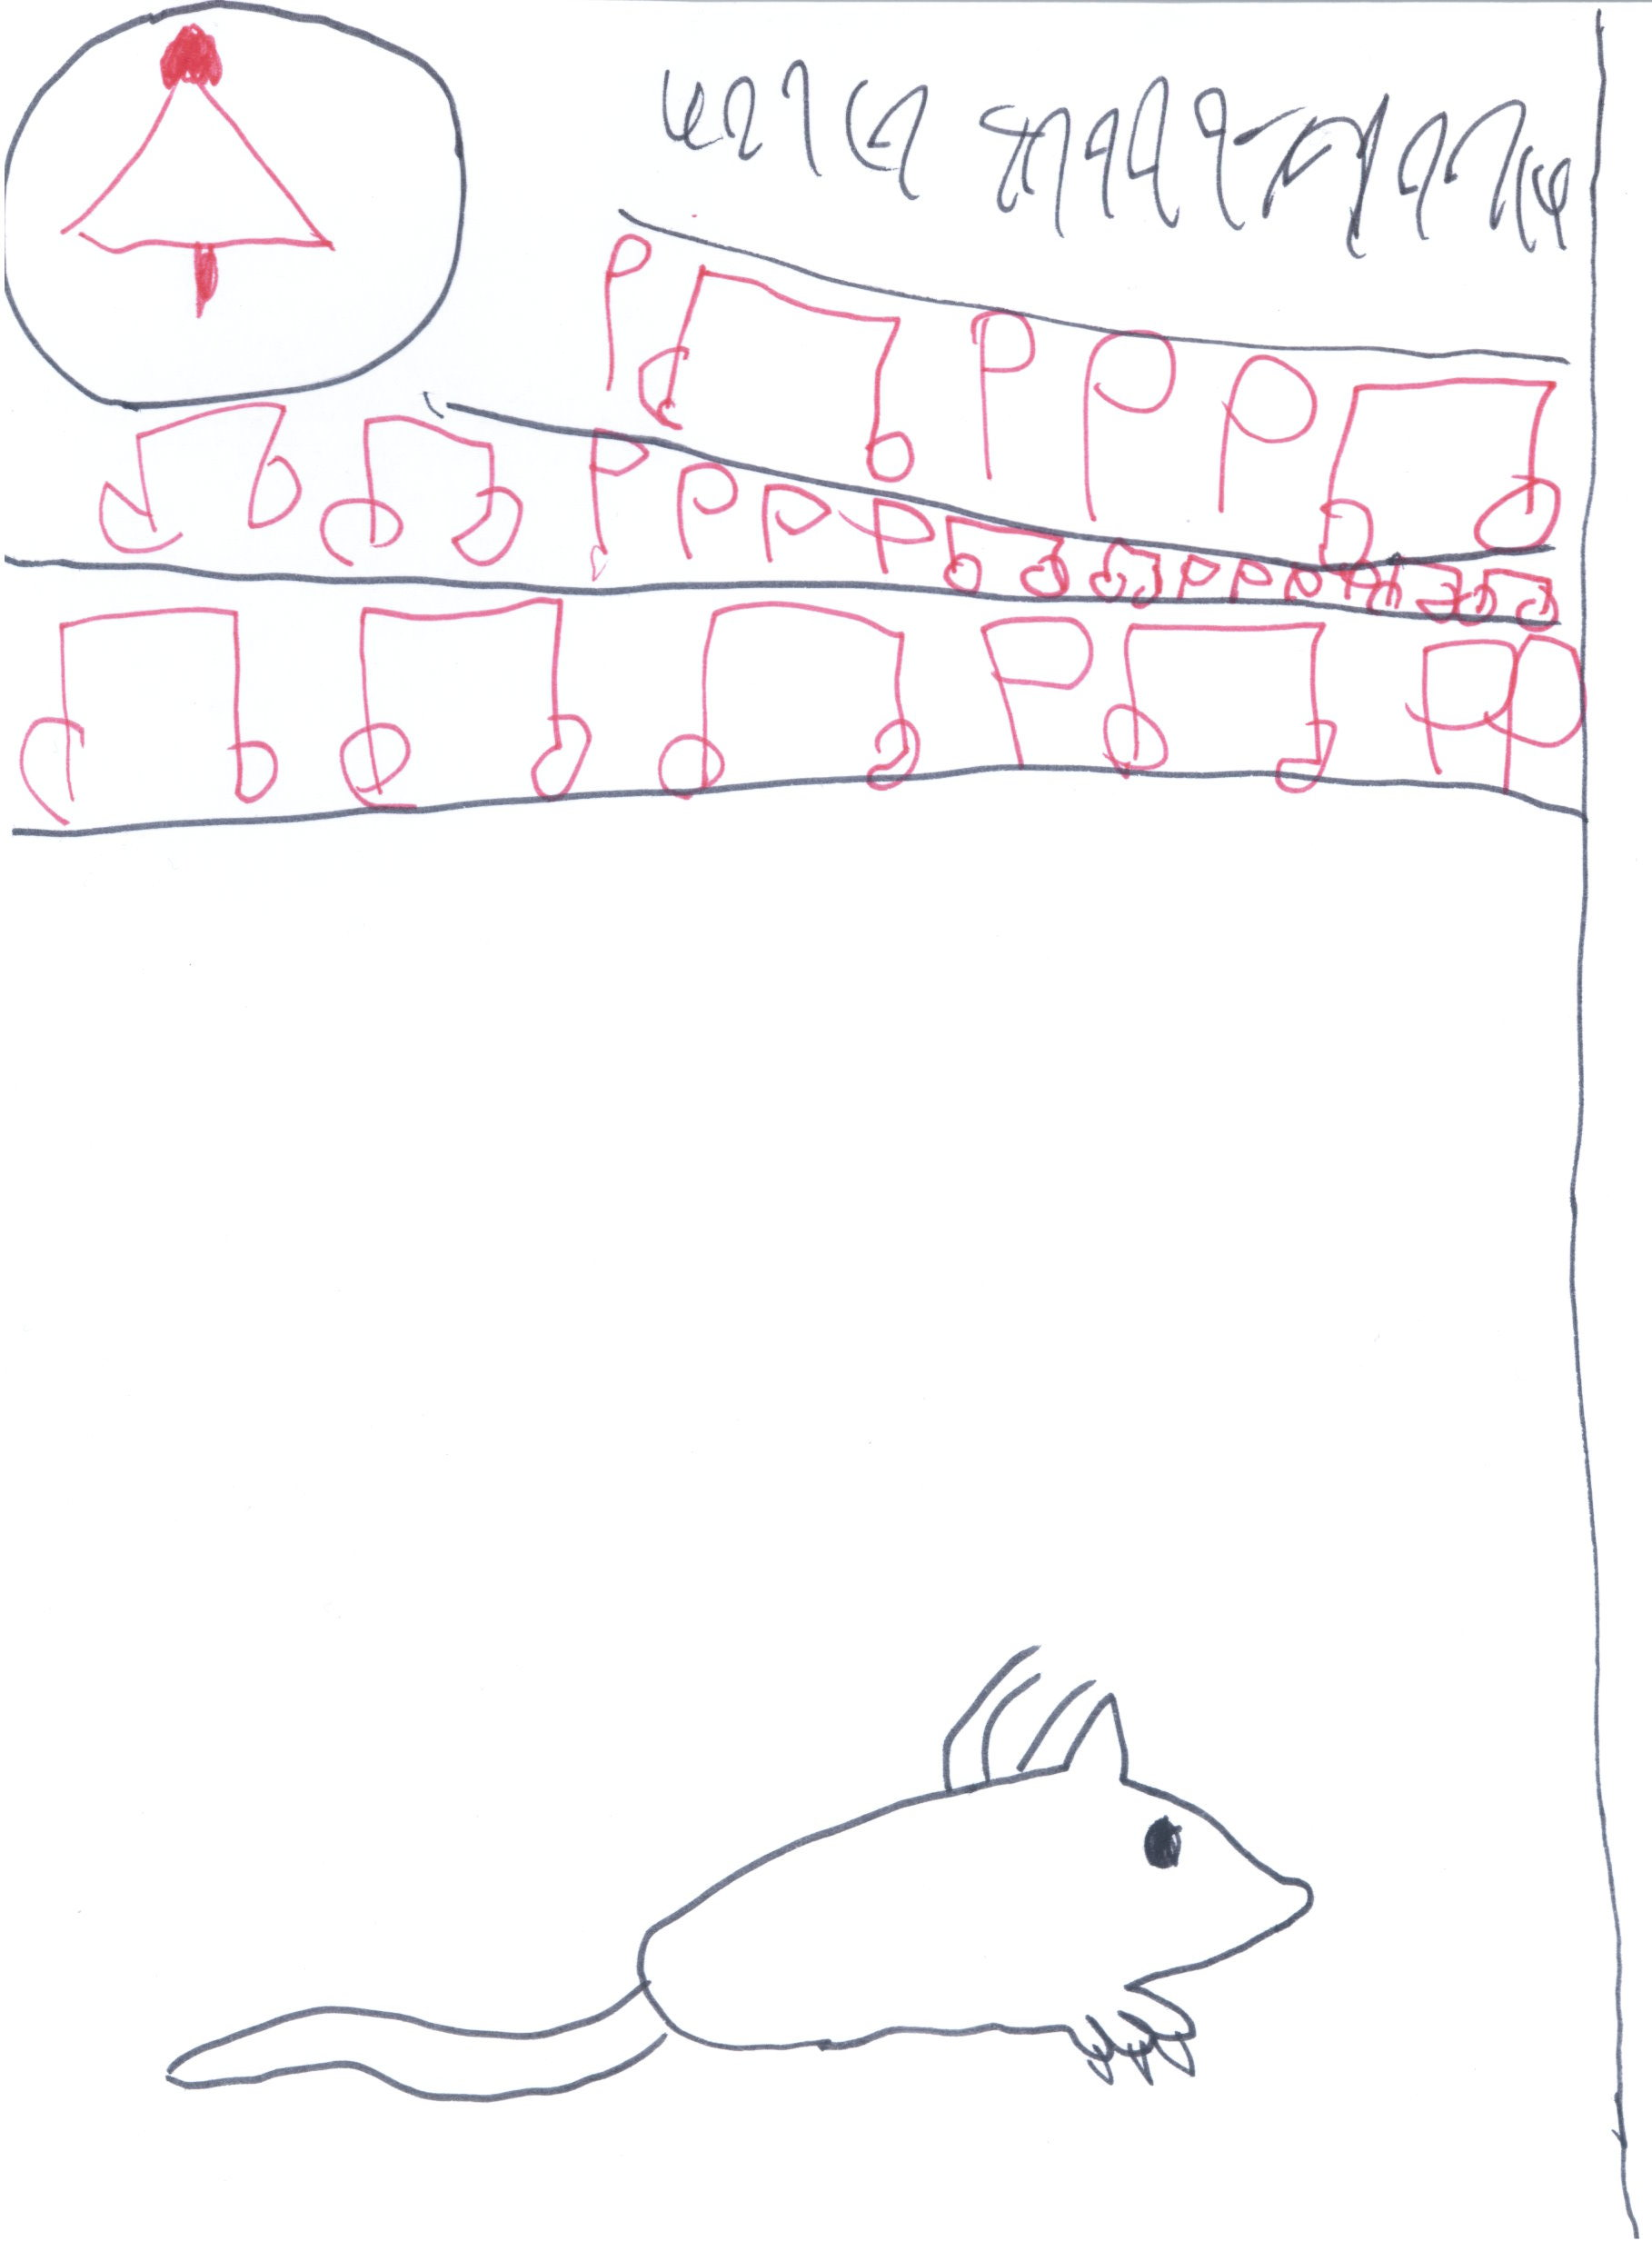
\includegraphics[width=.5\textwidth]{bilder/maus_2.jpg}
\end{floatingfigure}

Das Kind war aber gar kein richtiges Mäusekind, sondern eine gute Fee. Und weil sie Mitleid mit der Maus hatte, sagte sie zu ihr: \enquote{Du bist eine gute Maus, dass weiss ich. Du hast mir einmal dieses Holzpüppchen geschenkt obwohl du mich gar nicht kanntest, und deswegen will ich dir helfen. Leider bin ich keine der mächtigen Feen, die alle Wünsche erfüllen können, aber ich kann dir drei Mal einen guten Rat geben. Nimm dazu diese drei Federn. Wenn du eine auf die Hand legst, und in die Luft bläst, stelle deine Frage und ein Geist wird erscheinen und dir die Antwort geben.}

Die Maus wusste zuerst gar nicht, was für ein grosses Geschenk das war. Was nützen mir Ratschläge, dachte sie zunächst, wenn ich vor Hunger fast nicht denken kann? Aber dann kam der Maus ihre erste Idee. Warum nicht fragen, wo es heute feines Futter zu finden gibt? Und schon hatte sie eine Feder in der Hand. Aber halt, warum nicht gleich fragen, wo es heute und morgen etwas Leckeres gibt, dachte sie richtig. Die Maus wurde immer aufgeregter, als sie langsam verstand, was sie da von der Fee bekommen hatte. Denn noch besser konnte sie fragen, wo es eine Mühle so wie ihre gäbe, wieder mit einem Müller der sie in Ruhe liesse? Oder einen Ort, der war wie ihre Mühle, nur dass es noch feine Kleider umsonst gäbe?

So steigerte die Maus ihren Wunsch immer mehr, bis sie irgendwann zu dem Ergebnis kam, dass nur eine Frage geschickt sein könne. Sie nahm eine der Federn, legte sie auf ihre Hand, so wie es die Fee gesagt hatte und blies sie in den Himmel. Ein sanfter Windhauch nahm die Feder und liess sie steigen und steigen. Die Maus blinzelte ihr hinterher und fragte mit lauter Stimme: 

\enquote{Wie schaffe ich es, eine sehr reiche Maus zu werden?} Als die Feder gerade die Sonne zu berühren schien, antwortete eine ferne Stimme:

\enquote{Du kannst keine Körner sammeln, Du kannst keine Höhle bauen. Und doch bist Du geschickt in manchen Dingen. Erkenne was Du kannst! Aber bedenke: Nur wer bescheiden ist und im Sommer die kleinen Äpfel verschont, wird im Herbst grosse süsse Äpfel ernten können.} 

Die Maus hatte vor Aufregung ihre Barthaare gekräuselt. Enttäuscht von der Antwort, rollte sie die wieder auf, nur um sie gleich hängen zu lassen. Was sollte denn das bitte bedeuten? Sie hatte schon gehofft, einen Ratschlag zu erhalten, der besser verständlich wäre. Traurig senkte sie den Kopf. Ihr Blick viel auf einen dicken Ast und so begann sie zu nagen, nur um nicht so frieren. 

Da kam ein Mäusevater des Weges gelaufen und sah die kleine frisch genagte Babypuppe. 

\enquote{Die ist ja herrlich!}, rief dieser, \enquote{Guter Freund, seit Tagesanbruch bin ich auf der Suche nach einem Weihnachtsgeschenk für meine Kinder, sei so gut, und verkaufe mir deine Arbeit, ich möchte dir auch einen Gulden zahlen.}

\begin{figure}[hb]
\centering
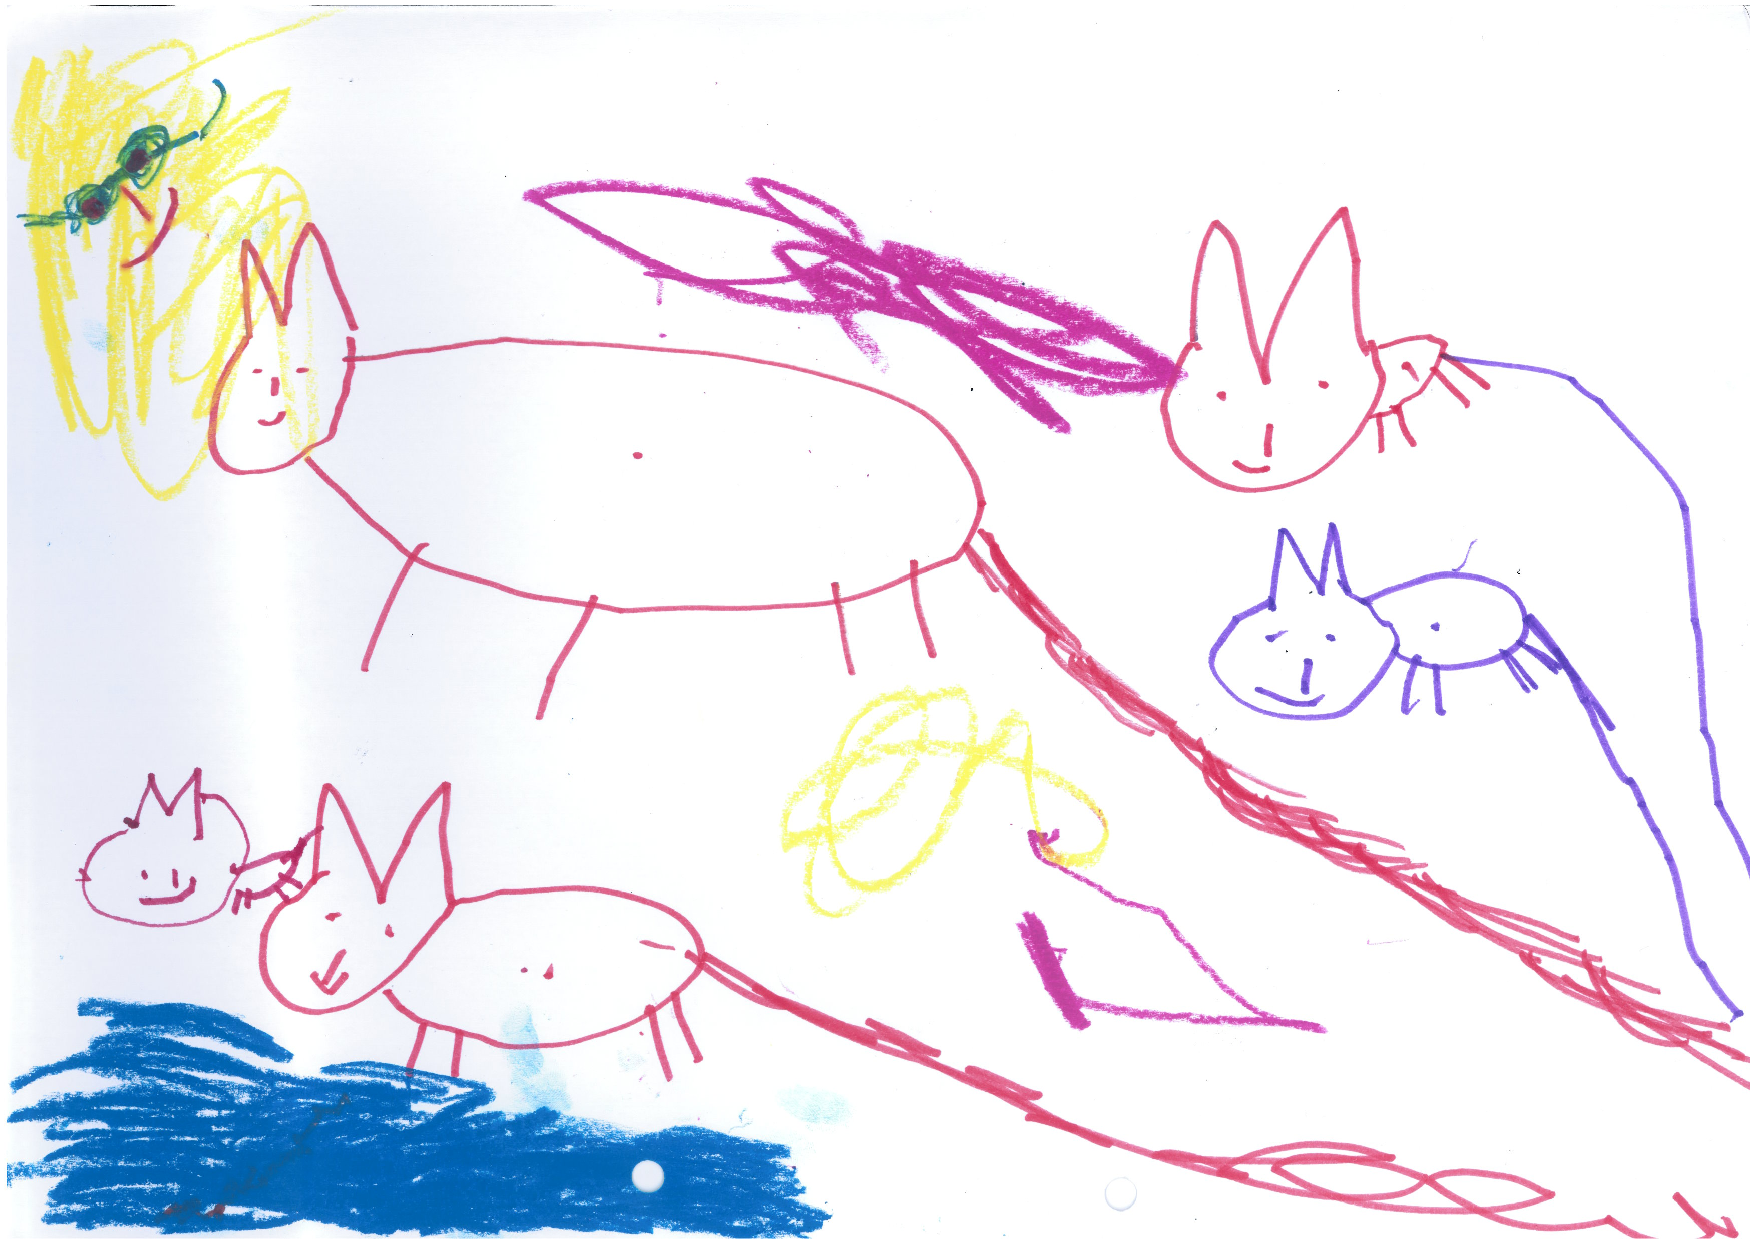
\includegraphics[width=.8\textwidth]{bilder/maus.pdf}
\end{figure}


Die Maus willigte natürlich sofort ein. Ein ganzer Gulden! Was man dafür alles für leckere Dinge kaufen konnte. Danke, liebe Fee, dachte sie, denn jetzt verstand die Maus den Ratschlag der Fee und wurde Puppenmacher. 

Mit dem ersten verdienten Gulden ging die Maus zum Krämer und bestellte sich den ersten Schweizer Käse in ihrem Leben. Gierig atmete sie den Geruch des alten Hobelkäses ein, als ihr gerade noch der zweite Teil des Rates der Fee einfiel. Bescheiden zu sein und sparen, hiess das wohl. Die Maus gab den teuren Schweizer Käse zurück, nicht ohne nochmals einen tiefen Zug des herrlichen Duftes inhaliert zu haben, und liess sich stattdessen vom Krämer ein trockenes Stück Brot geben. 

Mit dem gesparten Geld ging die Maus zum Holzhändler und kaufte sie ein schönes Stück edlen afrikanischen Holzes, ganz in schwarz. Der Holzhändler lachte zunächst, als er die verlumpte Maus sah, die auch noch vom teuersten Holz kaufen wollte. Als diese ihm aber fast einen ganzen Gulden auf den Tisch zählte, schüttelte er nur den Kopf und holte ein Stück Ebenholz. Die Maus begann zu nagen und nagte eine herrliche Büste einer schönen Mäusin. Sie klopfte an alle Türen des Dorfes und konnte die schwarze Schönheit endlich für acht Gulden an einen Kutschenbauer verkaufen.

Wieder sparte sie und kaufte Holz. Daraus nagte sie die schönsten Dinge. Spielzeug und Möbel, Statuen berühmter Mäuse und sonst noch allerlei. Damit zog sie von Haustür zu Haustür und erzielte immer viel mehr Geld, als das Holz gekostet hatte. Nach einem halben Jahr war sie es Leid die Leute zu besuchen und mietete sich ein eigenes Geschäft. Dort konnte sie einen grossen Vorrat an Nagwerk vorrätig halten, da konnte fast jeder etwas passendes finden.

So verging die Zeit und Maus wurde immer reicher. Die edelsten Käse waren eine Selbstverständlichkeit geworden und zwar reichlich. Sie hatte jetzt auch Gehilfen, denen sie gezeigt hatte, wie man nagen muss, das machten die jetzt für sie. Die Maus wurde immer fetter und fetter und fetter, bis sie fast keine Luft mehr bekam. Der herbeigerufene Arzt beschnüffelte die Maus von allen Seiten und prophezeite ein baldiges Herzversagen, wenn das mit der Bauchwachstum nicht schleunigst umgekehrt werden würde, die Maus also abnehmen solle. Aber viel Hoffnung habe er nicht, musste er einräumen.

Die Maus fühlte, dass es Zeit für die zweite Frage sei. Aber was genau sollte sie diesmal fragen? Wie sie ihre Gesundheit retten könne, war sicher eine gute Frage. Aber dann hatte sie nur noch eine Frage übrig und war es nicht sehr gefährlich, diese letzte Frage nicht optimal zu nutzen? Sollte sie nicht vielleicht besser fragen, was die beste letzte Frage sein könne? Möglicherweise war ja aber gerade die Frage nach der Gesundheit die beste Frage. Und dann hätte sie die letzte Frage verschenkt.

Die Maus dachte lange nach, doch konnte sie sich nicht entscheiden. Aber eine Entscheidung musste getroffen werden.  So nahm sie die zweite Feder und blies sie in die Luft. Die zweite Feder erreichte den Mond und gerade als sie diesen berührte, donnerte auch wieder die selbe Stimme wie beim ersten Mal.

\enquote{Also Maus, stelle deine Frage!} Die Maus erklärte ihr Problem, dass sie sich nämlich nicht entscheiden können.

Die Stimme seufzte, murmelte etwas davon, dass es so ja wohl nicht ginge, dass die Maus schon eine klare Frage formulieren müsse, dann aber sprach sie: \enquote{Die Lösung auf beide Fragen sind ein paar gute Schuhe.}

Wie das erste Mal auch, wurde die Maus nicht recht schlau aus diesem Rat. Schuhe? Was konnte das bedeuten? Schuhe hatte sie keine mehr, seitdem sie den eigenen Laden aufgemacht hatte. Wozu auch? Die Mäuse kamen zu ihr, auch der Holz- und der Käselieferant. Es hatte einfach keinen Grund mehr gegeben, das Haus zu verlassen. Dann verstand sie. Na klar, es war gemeint, dass sie laufen solle. Mit einem kleinen Spaziergang war es wohl nicht getan. Also schloss die Maus ihren Laden ab und hängte ein Schild ins Schaufenster, auf dem zu lesen war, dass die Maus jetzt einmal Ferien hat und auf Wanderschaft geht.

Wohin ist egal, dachte sie ganz richtig, Hauptsache laufen. Die Wege führten sie weit weg von zu Hause. Die ersten Tage kam sie dick und ungeübt wie sie war, kaum voran. Aber schon bald war sie wieder bei Kräften und lief eifrig nicht nur die Berge runter, sondern auch wieder hoch.

Die Maus wanderte viele Wochen. Abends klopfte sie an fremde Türen und bat um Unterkunft für eine Nacht. Als Gegenleistung nagte sie ihre berühmten Püppchen oder andere Dinge. So lernte sie die unterschiedlichsten Mäuse kennen. Mal schlief sie bei einer Familie, mal bei einer alten Witwe. Mal waren es wohlhabende Mäuse, mal arme. Eine Maus war sehr schlau und las viel, eine andere kaute den ganzen Tag auf einem Grashalm und machte nur das mindeste.

Alle, die die Maus traf, erzählte sie ihre Geschichte und wollte wissen, welche Frage sie wohl stellen würden. Vielleicht hatten die anderen Mäuse ja eine Idee.

\enquote{Ich würde gerne wissen, welches Mittel es gibt, dass meine Kinder mich einmal eine Nacht schlafen lassen.} wollte eine Mutter wissen. \enquote{Woher weiss ich, ob meine Freundin mich liebt?} war ein jugendliche Maus besorgt. \enquote{Wo bekomme ich den besten Preis für meine Ware?} gab sich ein Händler sachlich. Sehr weit kam die Maus und lernte sehr vieles kennen, fand aber nie, wonach sie suchte. Die richtige Frage für sich selbst.


\begin{figure}[ht]
\centering
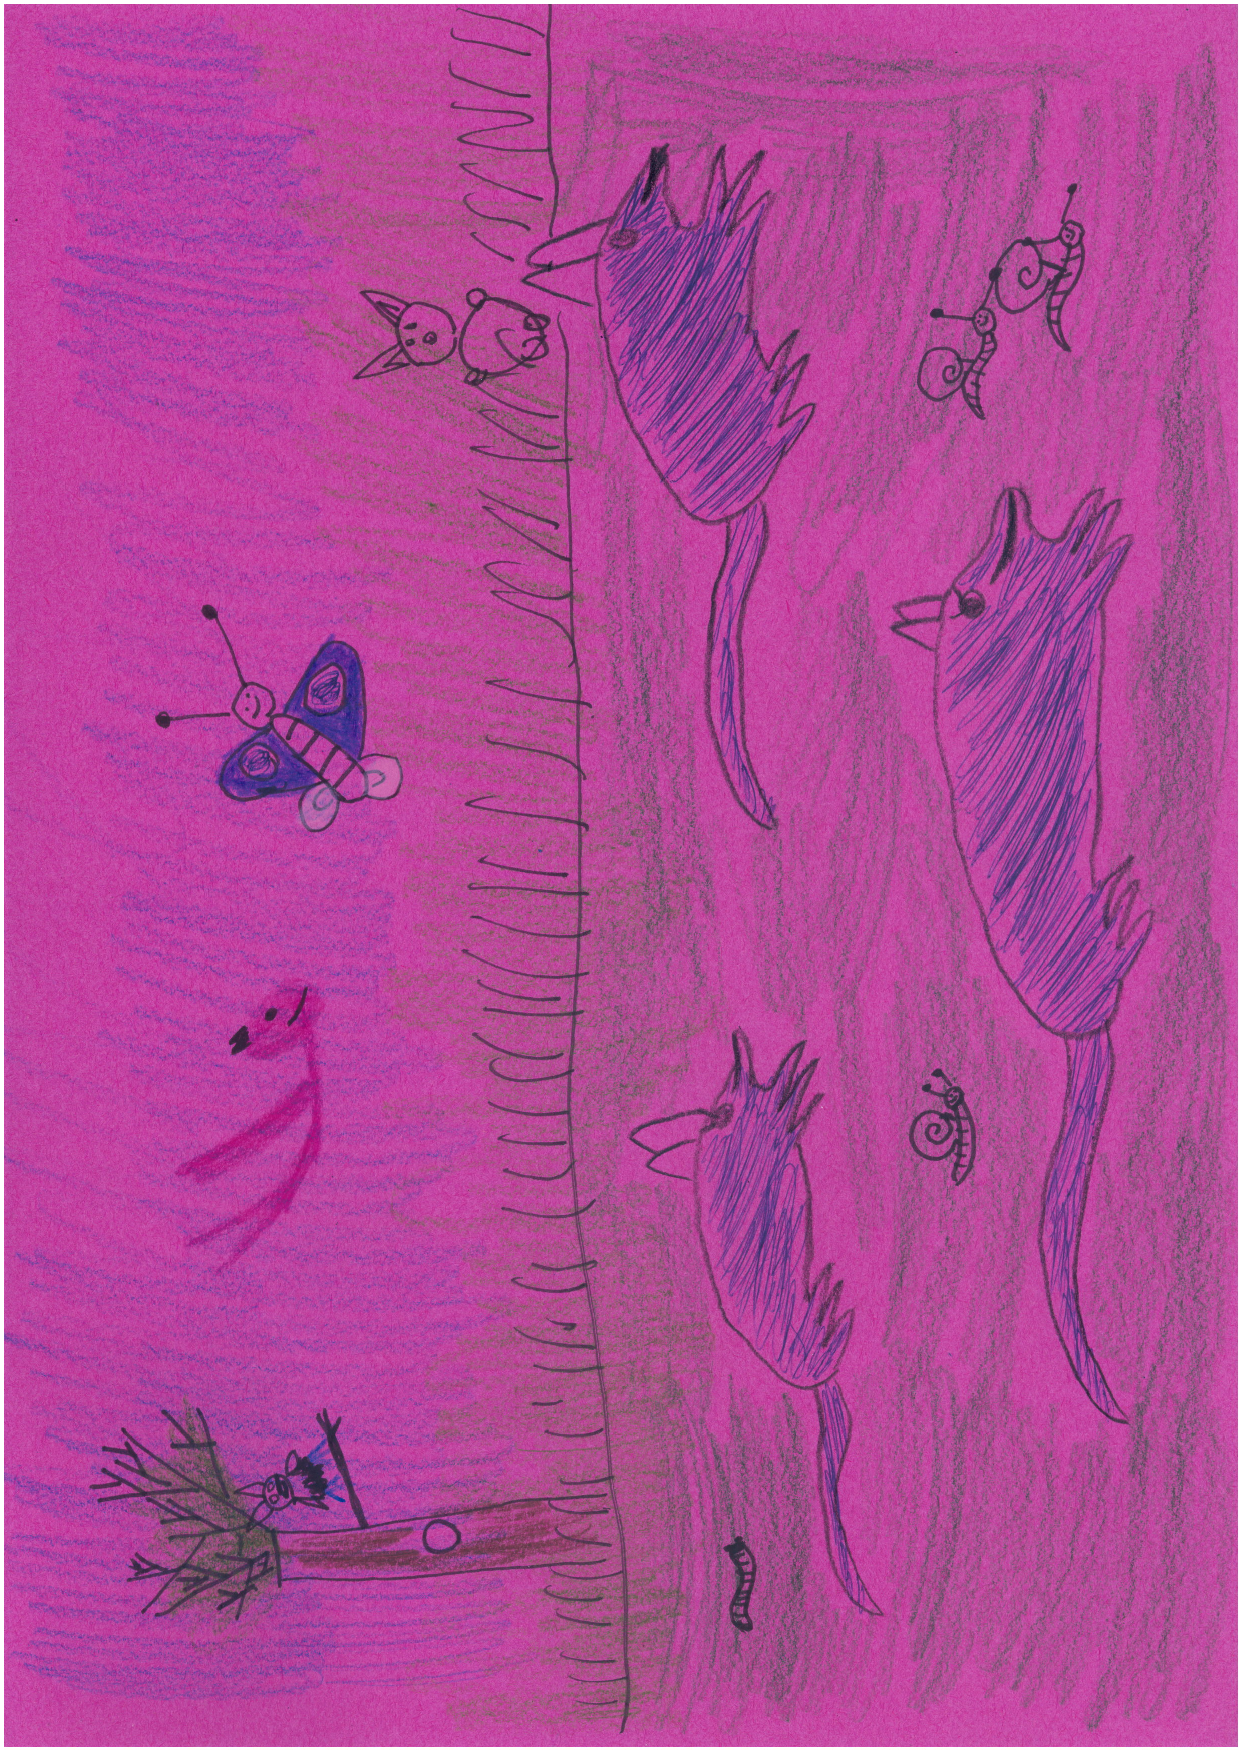
\includegraphics[angle=270,width=.7\textwidth]{bilder/maus_1.pdf}
\end{figure}

Jede Maus möchte etwas anderes wissen, dachte die Maus. Woher soll ich wissen, welches mein Wunsch ist? So kam sie zu einer sehr alten Mäusin. Die lebte ganz alleine gleich an einer schönen Lichtung im Wald. Auch hier hier bat die Maus um Unterkunft und bekam sie gewährt. 

\enquote{So so.}, sagte die alte Maus, \enquote{Du bist also auf der Suche nach der richtigen Frage? Ich kann dir nicht helfen, ich habe keine Frage.} 

\enquote{Aber Du möchtest doch bestimmt wissen, wie du wieder jung und schön werden kannst?} entgegnete die Maus.

\enquote{Nein, nein. Ich habe mein Leben glücklich und zufrieden gelebt. Ich habe vieles von dem, was ich mir gewünscht hatte, nicht erreicht. Aber ich habe es immer wieder versucht, also will ich zufrieden sein, mit dem was ich habe, und das ist nicht wenig. Ich habe mich und meine Kinder und Enkel, die mich regelmässig besuchen und die ich lieb habe. Ich habe genügend Futter für den Winter, was sollte ich wohl brauchen. Aber denk einmal nach. Du hast auf Deiner Reise sehr viele verschiedene Fragen gehört. Jeder hat etwas anderes gesagt, aber eigentlich haben alle das selbe gemeint.}

Die Maus lag die ganze Nacht wach und dachte über das nach, was die Alte gesagt hatte. Und als die Sonne aufging, hatte sie die Lösung.Das war es. Glück! Glücklich wollen die Mäuse sein, jede auf ihre Art, aber eben doch glücklich! Jetzt, wo die Maus die richtige Frage kannte, war sie sehr erleichtert und beschwinkt. Sie wollte Fragen, wie man glücklich wird! 

Sie kostete die Zeit aus. Bestimmt einhundert Mal nahm sie die Feder in den nächsten Tagen in die Hand und wollte sie in die Luft blasen. Aber irgendetwas sagte ihr, dass sie sich erst wirklich sicher sein sollte, dass das die richtige Frage ist. Erst ein paar Mal darüber schlafen, immerhin war es die letzte Frage.

Die Maus wanderte weiter und kam an einen Bach, da lebte eine schöne Mäusin. Vornübergebeugt versuchte sie ihre Wäsche im Fluss zu waschen, aber es gelang nicht recht, da sie ihre Pfote nicht richtig bewegen konnte und sie ausserdem furchtbar husten musste. Während die Maus der kranken Mäusin half, erklärte die, schon seit Jahren krank zu sein, aber kein Arzt wisse, wie man ihr helfen könne.

Die Maus fragte auch hier nach Unterkunft und bekam sie. Sie half der armen Mäusin und blieb sogar ein paar Tage, was sie sonst niemals tat. Sie merkte schnell, dass sie gar keine richtige Lust mehr hatte weiter zu reisen. Erst dachte sie, dass es daran liegt, dass sie ja jetzt wisse, welche Frage sie stellen will und ausserdem war vom dicken Bauch nichts mehr übrig. Sie strotzte nur so vor Kraft und Vitalität. Aber sie merkte schnell, dass etwas ganz anderes der Grund ist. Sie hatte sich in die kranke Mäusin verliebt und die wohl auch in sie.

Und am dritten Morgen ging die Maus zum Bach, nahm die Feder und blies sie in die Luft. Als die Feder so hoch war, dass sie über den Wolken schwebte, fragte die Maus, wie wohl der Mäusin zu helfen sei.

Die donnernde Stimme war wieder zu hören und diktierte ein langes Rezept für eine Arzenei. Und sie verordnete Bewegung und frische Luft. Nachdem die Maus den Trunk genau so gebraut hatte und die Mäusin ihn getrunken hatte, fragte die Maus, ob sie Lust hatte, mit ihr durch die Welt zu wandern. Und natürlich wollte die. So nahmen sich die beiden an die Hand und wenn sie nicht angehalten haben, dann wandern sie noch heute.

\chapter*{\FontH{\Huge Das Gespenst Jonathan}}
\addcontentsline{toc}{chapter}{Das Gespenst Jonathan}

\begin{quote}Vor drei Wochen habe ich zum ersten Mal in meinem Leben ein Gespenst gesehen. Klar, ich habe mir natürlich hin und wieder vorgestellt, dass es welche gibt, aber das meine ich nicht. Ich habe auch schon einmal gedacht, dass ich eines sehe, aber das war dann doch nur die frisch gewaschene Jacke von Frau Maier, unserer Nachbarin, die der Wind von der Leine gerissen hatte. Hab ich mich damals erschrocken! Die kam mir nämlich direkt entgegengeflogen und zwar nachts! Ich bin vor Schreck vom Fahrrad gestürzt und habe mir dabei die Hose zerissen. War das eine Aufregung und Mama wollte mir erst gar nicht glauben. Aber das will ich hier gar nicht erzählen, die Geschichte vom richtigen Gespenst Jonathan ist viel interessanter.  Das es Jonathan heisst, habe ich erst später erfahren. Aber ich will Euch mal die Geschichte von Anfang an erzählen, ich komme erst in der Mitte dazu.
\end{quote}

\lettrine[lines=2]{\color{red}K}{rrrawum.} Mit einem lauten krachen fällt die Rüstung von Ritter Odo von Gladez um. Die weisse Frau von Burg Lauenstein kommt durch die Wand gleich hinter der Rüstung geflogen und sieht sich den Haufen alten Blechs auf dem Boden an.

\enquote{Jonathan!} ruft sie, \enquote{Komm sofort hierher!} Mit gesenktem kommt auch Jonathan. Jonathan ist der Sohn der Weissen Frau, die eigentlich Otilia Brigitta Walburg Peternella von Abendberg heisst. Aber alle nennen sie die weisse Frau und das schon seit vierhundert Jahren. Sie ist nämlich ein Gespenst und die Mama von Jonathan, der natürlich auch eines ist. 

\enquote{Was soll ich nur mit Dir machen?} seufzt die Mama. Andauernd wirft Jonathan etwas um. Er passt einfach nicht auf, wenn er zu schnell durch die Wände geflogen kommt und nicht merkt, dass in dem Raum zum Beispiel eine Vase oder Kleiderständer steht. Gespenster können nämlich nur durch Wände fliegen, durch andere Sachen nicht. Und Jonathan war eben ein besonders schreckhaftes Gespenst. Immer wenn er glaubt, dass Menschen in der Nähe sind, nimmt er Reissaus und saust durch Burg Lauenstein, um sich zu verstecken. Besonders vor Kindern hat er furchtbare Angst. Die sind immer laut und frech und ärgern sich gegenseitig. 

Burg Lauenstein müsst ihr wissen, ist eine alte Burg. Tagsüber kommen Besucher aus der Umgebung und sehen sich an, wie die Menschen früher so gewohnt haben. Und zu einer alten Burg gehören eben auch Gespenster, die man allerdings nie am tage sieht und auch Nachts nur, wenn man sehr viel Glück hat. Seitdem irgendjemand mal auf die Idee gekommen ist, zu behaupten, dass Gespenster ganz gefährlich sind, haben sie angefangen, sich in den Kellern und Türmen oder wenigstens den Truhen der alten Burgen und Schlösser zu verstecken. Die allermeisten haben sich aber in Büchern versteckt und leben jetzt nur als Geschichte weiter. Eigentlich kenne ich kein Gespenst mehr, dass nicht nur in Büchern lebt, die weisse Frau und ihr Sohn Jonathan sind vielleicht die letzten.




\chapter*{\FontH{\Huge Der kleine Pirat Winnimon}}
\addcontentsline{toc}{chapter}{Der kleine Pirat Winnimon}
\section*{\center $\skull$ Die Prüfung $\skull$}
\lettrine[lines=3]{\color{red}W}{ie} jeder andere Pirat auch, war Winniemon nicht schon immer ein Pirat. Genau wie du und ich war er zunächst ein kleiner Junge, der höchstens einmal mit dem Boot seines Opas zum Angeln auf dem Meer gewesen ist. 

\todo{Aye. Dorf der Waisen. Piratengesetze-Mitspracherecht, Spanier, Klabautermann, Jolly Roger, Krähennest, Kombüse, Smutje, Papagei, Seemannsknoten, Bukanier}
Aber auch das war er nicht besonders oft, denn Winnimon hatte ein Problem, für das er sich sehr geschämt hat. Er konnte nicht schwimmen! Piraten müssen aber schwimmen können, das ist klar. Piraten müssen nämlich ständig Mutproben machen, da kann es schon einmal vorkommen, dass man mit verbundenen Augen und einem Messer im Mund auf der Reeling balancieren muss. Und wenn man dann den kleinsten Fehler macht, liegt man im Meer.

Wenn man nicht schwimmen kann, sollte man sich lieber einen anderen Beruf aussuchen. Das kam für Winnimon aber nicht in Frage. Undenkbar! Der Vater war ein Pirat und sein grosser Bruder war auch einer. Und was viel wichtiger war: alle seine Freunde wollten Pirat werden. Und die konnten schwimmen, die brauchten sich keine Sorgen zu machen.

Wenn man auf einem Piratenschiff anheuern möchte, muss man drei Prüfungen bestehen. Erstens muss man fluchen können wie ein alter Papagei. Das klappte bei Winnimon ausgezeichnet, jedenfalls fand das seine Mutter, die aber allgemein nicht viel für Flüche übrig hatte. 

\enquote{Du dreifach stinkender Pups einer blinden Robbe} war Winnimons Lieblingsfluch. Den hatte er erst einmal gesagt, als grosser Bruder ihm einmal zum Frühstück eine leere Eischale hingesetzt hatte. Die Mutter hätte ihm fast eine Ohrfeige gegeben, was aber ein gutes Zeichen war. Denn seitdem wusste er, welchen Fluch er zur ersten Piratenprüfung fluchen würde. Den hatte er lieber nicht noch einmal geflucht, nicht dass ihm den noch jemand von seinen Freunden klaut!

Die zweite Prüfung war auch nicht so schwer. Man musste lesen und schreiben können. Erstens musste man der Mutter eine Flaschenpost schicken können, falls zum Beispiel die Socken so alt waren, dass sie neue schicken musste oder wenn man einfach Heimweh hatte. Das darf man sogar als Pirat haben, der gerade durch ferne Meere kreuzt. Und man musste natürlich Schatzkarten lesen können. Wenn da steht \enquote{Der Schatz liegt auf der Insel Woladimadudistan} ist das schon besser, sonst muss man den Schatz auf allen Inseln suchen und von denen gibt es viele. Aber Winnimon war zwar nicht so schlau wie die lange Druda aus seiner Klasse, aber Lesen und Schreiben klappten prima. Kein Problem also, die zweite Piratenprüfung.

Es blieb nur die Sache mit dem Schwimmen. Nicht dass Winnimon es nicht immer wieder einmal probieren würde. Aber er zappelte nur, der grosse Bruder lachte, der Vater war ärgerlich und nach dem zweiten Schluck Wasser, dass er unfreiwillig getrunken hatte, gab er immer auf. Wie machten das die anderen bloss? Wen er probierte, nicht mehr mit den Beinen auf dem Boden zu stehen, ging der Kopf automatisch unter Wasser. Schrecklich! Er hatte gar keine Zeit, überhaupt nur einmal einen Schwimmzug zu probieren.

In dem kleinen Dorf, in dem er wohnte, herrschte grosse Aufregung. Ein Piratenschiff hatte sich angekündigt, in drei Wochen schon sollte es da sein. Es wurden Jungen gesucht, die mit auf See wollten. Und Winnimon wollte. Und wie er wollte! Pirat sein, das ist das Grösste! Sofort machte er sich auf zum Meer, schwimmen üben. Noch drei Wochen, bis dahin musste das klappen, unbedingt. 

Am Strand waren schon die anderen Jungen versammelt, auch die, die nicht Pirat werden wollten. Sie hatten aus Brettern ein Floss gebastelt und spielten natürlich Pirat. Sie sprangen von Floss ins Wasser und schwammen um die Wette. Winnimon zog seine Badehose und watete vorsichtig ein paar Schritte ins Meer. Die Wellen schwapptem ihm gegen den Bauch. Er wusste nicht einmal, wie er anfangen sollte zu üben. Er wartete auf ein Tal zwischen zwei Wellen und kniete sich hin. Aber schon spülte die nächste Welle ihn im hohen Bogen ans Ufer zurück. 

Den anderen war das traurige Schauspiel natürlich nicht entgangen. Lachend und schreiend kamen sie angerannt und hänselten Winnimon.

\enquote{Seht Euch mal den an, der Schwimmt ein Sack voller Steine!} war noch das Harmloseste. Obwohl Piraten nie weinen, kullerten Winnimon ein paar Tränen über die Wangen. Nicht weil die anderen ihn gehänselt haben, das war nicht so schlimm, so was kommt vor, er hat ja auch schon mitgemacht. Das Schlimme war, dass sie ja Recht hatten. Er schwamm tatsächlich genau so wie ein Sack voller Steine: immer direkt nach unten.

Eine Hand legte sich auf seine Schulter. Die lange Druda stand hinter ihm. An jedem anderen Tag wäre Winnimon vor Scham im Erdboden versunken, wenn ein Mädchen ihn weinen sieht, aber heute war ihm alles egal. Schluchzend erklärte er ihr, warum er so weinen musste. Druda überlegte. 

\enquote{Also pass auf} sagte sie. \enquote{Ich bringe dir das Schwimmen bei. Aber Du musst dann auch etwas für mich tun. Versprichst Du das?}

Winnimon zögerte keinen Augenblick. \enquote{Alles, was Du willst!}

\enquote{Na gut, dann komm morgen früh zum Waldrand. Und bring zwei Rumfässer und ein Seil mit.}

Ausgerüstet mit den verlangten Dingen und einer frisch gewaschenen Badehose stand Winnimon schon am Waldrand, bevor es hell wurde. Druda kam pünktlich zum Sonnenaufgang und hatte nicht vergessen, etwas zum Essen mitzubringen. Als erstes sträkten sich die beiden, dann gingen sie zu dem kleinen Waldsee, der ein bisschen versteckt war.

\todo{Zeitformen anpassen}
\enquote{Hier wirst du schwimmen lernen} sagt sie. \enquote{Das Wasser hier ist ruhig, da kann man besser üben. So, und jetzt binden wir den Strick zwischen die beiden Fässer, aber so, dass noch etwas Platz dazwischen ist.}

Knoten konnte Winnimon schon sehr gut und so dauerte es nicht lange, bis er fertig war. Die Fässer sollten als Schwimmer dienen, er selbst legte sich auf die Seile dazwischen. So konnte er nicht untergehen. Druda zeigt ihm mit viel Geduld wie man schwimmt. Die Beine wie ein Frosch und die Arme wie ein Pfeil nach vorne und wie ein Bogen nach hinten.

Noch am selben Tag klappte das schon ganz gut und einen Tag später liessen sie die Fässer weg. Winnimon schwamm jeden Tag Und jedes Mal ein bisschen besser. Nach der ersten Woche waren beide zufrieden. Winnimon konnte schwimmen wie ein Fisch und ebenso gut tauchen.

Druda meinte: \enquote{Das Letzte, was Du noch lernen musst, ist einen ordentlichen Kopfsprung zu machen. Aber bevor ich dir den zeige, erinnere ich dich daran, was du mir versprochen hast. Jetzt musst du mir helfen.}

\begin{figure}[hb]
\centering
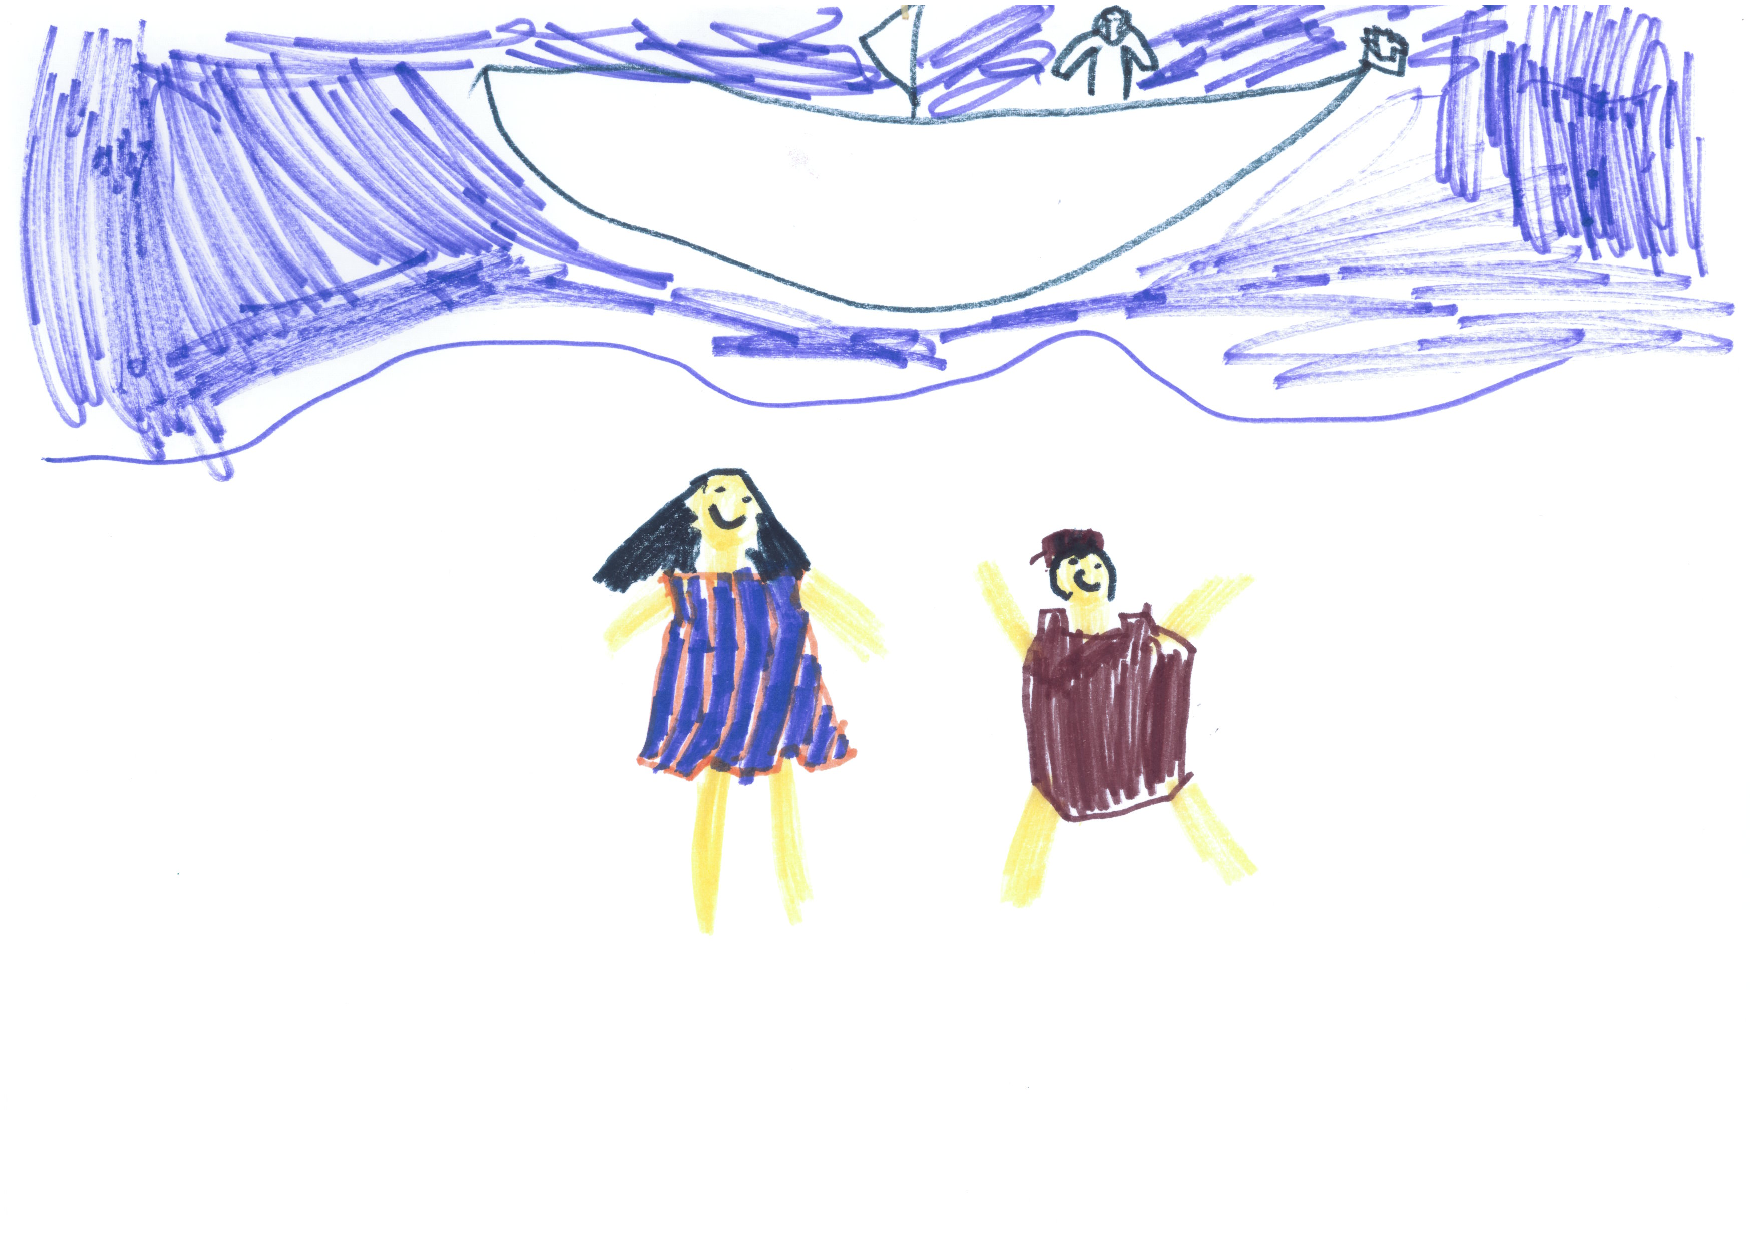
\includegraphics[width=.7\textwidth]{bilder/pirat1.pdf}
\end{figure}

Winnimon blickte fragend. Sie holte tief Luft und sagte: \enquote{Ich kann nicht fluchen. Mir fällt einfach kein Fluch ein. Du musst mir den besten Fluch verraten, den du kennst!}

\enquote{Aber warum willst du denn fluchen können?} Winnimon blickte fragend. \enquote{Du willst doch nicht etwa\dots?}

\enquote{Aber natürlich will ich auch Piratin werden! Meinst du ich will mein ganzes Leben hier verbringen? Ich will auch raus und die Welt sehen. Und jetzt hab ich dir geholfen, jetzt musst du mir helfen!}

Winnimon sah das sofort ein. Ihm ging es ja genauso. Und er zögerte nicht lange und verriet Drude seinen Lieblingsfluch. Das war er ihr schuldig, da gab es keine Frage. Ihm würde schon etwas einfallen.

Als beide zurück im Dorf waren, merkten sie gleich, dass etwas nicht stimmt. Vorbei am Haus von Winnimon sahen sie es auch schon. Ihm Hafen waren riesige Segel zu sehen und ganz oben auf dem höchsten Masten wehte die schwarze Fahne mit dem Totenkopf. Die Piraten waren da!

Sofort liefen die beiden hinunter zum Hafen. Das ganze Dorf hatte sich schon versammelt. Ein dicker Pirat stand in der Mitte der Menschenmenge auf einem Fass und rief:

\enquote{Liebe Leute. Mein Name ist Francisco San. Ich diene unter Barnabas Rotwild als erster Leutnant auf der Drachenblume, dem grössten Piratenschiff weit und breit. Wir sind gekommen, um zu fragen, ob jemand hier an Bord anheuern will. Wir nehmen zwei Schiffsjungen auf. Kommt mit uns, lernt die Welt kennen und werdet reich oder geht mit uns unter. Ihr alle kennt die drei Prüfungen. Aus all denen, die sie bestehen, nehmen wir zwei von euch auf. Freiwillige, tretet vor! Lang leben die Piraten!}

Alle Jungen und Mädchen waren sofort sehr aufgeregt, alle wollten mit. Nachdem sich die ersten getraut hatten vorzutreten, gaben sich auch Winnimon und Drude einen Ruck und stellten sich neben die anderen, alle in eine Reihe. Das alles so schnell gehen würde, hätten sie ja nie gedacht.

\enquote{Na dann wollen wir mal sehen.} Leutnant Francisco San schritt langsam die Reihe der Jugendlichen ab und zwirbelte dabei seinen Bart. \enquote{Ihr nehmt euch jetzt alle einen Stift und ein Stück Papier von dort drüben und schreibt folgende Wörter auf: Schatztruhe, Gewitter, arbeiten und Papagei.}

Die Prüfung war nur für zwei Jungen und ein Mädchen ein Problem, die ohne zu diskutieren den Stift hinlegten und aus der Reihe der Jugendlichen zurücktraten. Die waren schon durchgefallen. 

Bei der nächsten Prüfung, dem Fluchen, ging es sehr schnell zu. Jeder musste sich auf das Fass stellen und einmal so laut fluchen wie er konnte. 

\enquote{Dreibeiniger Hund}, \enquote{Vierauge}, \enquote{Vogelscheuche}, das waren so die Flüche die man hören konnte. Aber der Leutnant war nicht zufrieden. Die Flüche hätten alle schon einen längeren Bart als Kapitän Rotwild. Und wenn man so lange auf See ist und man immer die selben Flüche hört, wird einem echten Piraten sofort langweilig. Dann kamen Drude und Winnimon an die Reihe. Drude bestand den Test sofort mit mit dem {\it dreifach stinkenden Pups einer toten Ratte}. Sie war Winnimon sehr dankbar, denn mehr als Schwachkopf, aber da musste sie selbst zugeben, dass das sehr langweilig ist.

Winnimon brachte erst kein Wort heraus. So lange hatte er sich darauf verlassen, einen prima Fluch zu haben, dass er sich keinen neuen überlegt hatt. Wie angewurzrlt stand er auf dem Fass, aber dann brach es aus ihm heraus:

\enquote{Eitrige Warze am Bauch einer toten Ratte}. Der Leutnant lachte und sagte bestanden.

Danach waren nur noch drei Jugendliche im Rennen. Drude, Winnimon und ein weiterer Junge. Einer von denen die immer über Winnimon gelacht hatte, wenn der versucht hatte zu schwimmen. Er fühlte sich deswegen auch schon siegessicher, sprang gleich ins Meer, schwamm ein paar Züge und kam mit triumphierenden Lachen wieder aus dem Wasser. Drude machte es ihm nach. Jetzt waren alle Augen auf Winnimon gerichtet. Der sprang aber nicht gleich ins Wasser, sondern kletterte erst auf das Schiff, stellte sich auf die Reeling und blickte nach unten. Das Wasser war jetzt doch viel weiter weg, als er gedacht hatte. 

Die anderen Jungen fingen schon an zu lachen, da sprang Winnimon im weiten Bogen und mit Kopf voran in die nächste Welle. Als er wieder hoch kam, hatte er zwar Wasser geschluckt, liess sich aber nichts anmerken und schwamm zurück an Land. Alle klatschten, damit hätte niemand gerechnet.

Nur der Leutnant war unzufrieden. \enquote{Wir wollten ja nur zwei mitnehmen.} sagte er. \enquote{Na gut, dann stelle ich jedem von euch eine Frage. Du}, und dabei zeigte er auf Winnimon, \enquote{Wie heisst unser Piratenschiff}.

\enquote{Drachenblume!} Das war leicht für Winnimon. Er hatte schon so oft von der berühmten Drachenblume reden hören, er wusste alles über dieses Schiff. 

\enquote{Und Du}, diemal zu dem Jungen gewand \enquote{Was für ein Schiffstyp ist die Drachenblume?} Der Junge wurde bleich und ganz verlegen. Er wusste es nicht.

\enquote{Eine Galeone} rief Drude. Na klar, Drude wusste eigentlich fast alles. Sie war die beste der Klasse gewesen. 

\enquote{Damit ist es entschieden!} rief der Leutnant. \enquote{Ihr beiden kommt mit! Und wie es der Piratenbrauch verlangt, geht ihr sofort an Bord. Ihr dürft euch nicht nochmals umdrehen und von niemandem verabschieden. Euer altes Leben ist vorbei, ihr seid jetzt Piraten an Bord der Drachenblume.}

Winnimon und Drude hatten Tränen in den Augen. Das war jetzt doch alles sehr schnell gegangen. Aber sie bleiben tapfer und drehten sich nicht nochmals um, als sie auf das Schiff gingen. Sie hörten nur wie die Dorfbewohner klatschten. Als sie das Schiff betraten, fingen die Piraten an, alte Piratenlieder zu singen.
\begin{verse}\it
15 Mann auf eines Toten Truh'\\
Johoho und ne Buddel voll Rum\\
Versoffen und beim Teufel ist die ganze Crew\\
Johoho und ne Buddel voll Rum\\
\end{verse}
\section*{\center $\skull$ Die ersten Tage als Pirat $\skull$}

Die Wellen brandeten unaufhörlich gegen die Drachenblume. Nicht eine Minute lag das Schiff ruhig im Wasser. Die letzten sind hart gewesen. Winnimon war seekrank geworden und musste sich die ganze Zeit übergeben. Jetzt ging es aber schon besser, jedenfalls dem Bauch. Der Smudje hatte die ganze Zeit neben ihm gesessen und das wildeste Seemannsgarn gesponnen. So sagt man, wenn Seeleute Geschichten erzählen, die gar nicht wirklich stimmen. Jedenfalls bildete sich Winnimon ein, dass die Geschichten wohl nicht stimmen können. Vor riesigen Kraken hatte der Smudje erzählt, die ganze Schiffe in die Tiefe reissen konnten. Und von schlimmen Piratenkapitänen, die noch nach ihrem Tod als Gespenster andere Schiffe überfielen. Von Sirenen, die so schöne Stimmen hatten, dass wenn man sie hört, unbedingt zu ihnen hinsegeln möchte, aber dann gegen ein Riff fährt und versinkt. So Geschichten eben. Dazu hatte der Smudje immer laut gelacht und sich Trockenfleisch mit seinem riesigen Messer abgeschnitten.

Winnimon lag in seiner Hängematte im Achterdeck und wollte sich kurieren, als die Schiffsglocke geläutet wurde. Alle Mann an Deck, hiess das. Ein Sturm war aufgezogen, da wurden alle Hände gebraucht. Winnimon musste an Leinen ziehen und Taue tragen, hier etwas festbinden und dort etwas holen. Viele Stunden dauerte der Sturm. Er hatte gar keine Zeit, Angst zu haben. Die anderen Piraten machten nicht den Eindruck, als ob etwas Besonderes vor sich ging. Als der Sturm endlich vorbei war, und alle irgendwo an Deck sassen und sich ausruhten, stellte sich Kapitän Barnabas Rotwild stellte sich auf die Brücke und rief mit wuchtiger Stimme:

\enquote{Männer, Frauen. Ich danke euch für eure Arbeit während des kleinen Sturms.}

Von wegen klein, dachte Winnimon.

\enquote{Wie ihr wisst, haben wir zwei Landratten an Bord gehabt. Ich glaube, nach diesem Sturm sind sie echte Seeleute geworden!} Dabei blickte er lachend zu Winnimon und Drude.

\enquote{Jetzt müssen wir nur noch Piraten aus ihnen machen. In zwei Tagen erreichen wir die Insel Pingelap. Auf Pingelap liegt ein Schatz, dass weiss ich. Die beiden Neuen sollen sich ein Boot nehmen und den Schatz bergen. Dabei werden sie auf sich allein gestellt sein. Haben sie den Schatz, sind sie vollwertige Piraten. Haben sie ihn nicht, lassen wir sie nicht wieder an Bord.}

Winnimon war bleich geworden und Drude auch. Sie fassten sich an die Hand und flüsterten \enquote{Wir schaffen das!}







Winnimon klatschte mit einer Hand nach einer Fliege. 

\enquote{Harrr!} hörte er hinter sich den alten Smudje schnaufen. ``Das ist nicht gut, sage ich, wenn einer jemanden tötet, der schlauer ist als er selbst!''

Winnimon wusste erst gar nicht, was der Smutje meinte. Er hatte ja noch nie jemanden getötet. ``Die Fliege meine ich, Du Grünspan''

Und noch bevor Winnimon etwas erwedern konnte, erklärte der Smutje: ``Auch bei Fleigen gibt es Mann und Frau, sonst könnte es keine kleinen Fliegen geben. Kannst Du die unterscheiden?'' 

``Ähhm''

``Siehst Du, und Fliegen können das. Alle. Sie wissen also mehr als Du.''



  \hfill {\color{red}\decofourleft}

\chapter*{\FontH{\Huge Der weisse Adler}}
\addcontentsline{toc}{chapter}{Der weisse Adler}
\lettrine[lines=3]{\color{red}J}{a}, Johann war eitel. Ihr werdet sagen, dass das nicht schön ist, aber so ganz unrecht hatte er nicht. Schön war er schon, der Johann. Denn Johann war der einzige weisse Adler weit und breit. Die anderen waren braun oder grau, wie Adler eben so sind. Auch schön, aber nicht so speziell wie Johann und oft ist es ja gerade das Spezielle, was wir als besonders schön oder manchmal auch als besonders hässlich empfinden. Und die anderen Adler mussten zugeben, dass das besonders reine Weiss seiner Federn tatsächlich sehr schön war. Und so nahm es Johann niemand übel, dass er so eitel war. 

Johann tat das aber gar nicht gut. Er wurde beinah von Tag zu Tag ein bisschen eitler. 

\enquote{Ha, ihr seht ja alle so schmutzig aus, mit euren braunen Federn, als ob ihr gerade in den Dreck gefallen wärt.}, rief er den anderen zu. Aber auch das war schon bald unter seiner Würde. Mit nach oben geschobenem Schnabel zog er seine Kreise in der Luft. Erhaben fühlte er sich und auserwählt vom Schicksal. Mit Verachtung blickte er auf die anderen Adler herab. Es dauerte nicht lange, da redete er sich sogar ein, der König der Adler zu sein. Und so benahm er sich auch.

Eigenartig war, dass die anderen Adler ihm glaubten. Sie dachten, weil Johann so Einzigartig aussah, müsse er wohl auch etwas besonderes sein. Und wer so besonders ist, ist sicher dazu bestimmt, der König zu sein. Also brachten sie ihm Mäuse, wenn er Hunger hatte und erfüllten ihm auch sonst alle Wünsche. Ein paar wenige Adler, die ihm besonders viele Mäuse brachten, standen in der Gunst von Johann weit oben. Sie bekam zur Belohnung von ihm eine weisse Feder geschenkt. Und weil Johann die nur selten verschenkte, waren diejenigen, die eine hatten, auch etwas besonderes und genossen bei den anderen Adlern hohes Ansehen. 

So ging es einige Jahr ganz gut. Johann war der König, er hatte seine treuen Freunde und konnte regieren wie er wollte. Nicht dass er das sehr ausgenutzt hätte. Eigentlich war er nur etwas faul und liess sich gerne bedienen. Hochnäsig zog er seine Kreise am Himmel.

Ein Adler-Sprichwort sagt, dass wer hoch steigt, auch tief fällt. Das habt ihr vielleicht schon einmal gehört, bei uns Menschen gibt es das ja auch. Und so erging es auch Johann. Eines Tages kam er auf die Idee, dass ein König auch einen Thron brauche. Aber was wäre denn gut genug, ein Thron für den König der Lüfte zu sein? Die Sonne war zu heiss. Der Mond war zwar schön, aber mal war er gross und rund und dann wurde er immer schmaler. Das passte Johann gar nicht und auch das blasse Gelb gefiel ihm nicht. Als einmal jemand vorgeschlagen hatte, er möge sich doch auf eine Wolke setzten, war er beleidigt.

\afterpage{
    \begin{figure}
        \thispagestyle{empty}
        \centering
        
\includegraphics[width=\textwidth]{bilder/adler.pdf}
    \end{figure}
    \clearpage
}


\enquote{Die Wolken sind für den gemeinen Adler, nicht aber für ihren König.} Und so blieb nur der Regenbogen übrig. Der war aber tatsächlich besonders gut geeignet! Die herrlich leuchtenden Farben passten wunderbar zu den weissen Federn unseres Johann. 

Zufrieden mit seiner Wahl beäugte Johann den Regenbogen von allen Seiten und beschloss, dass hier sein Thron sein soll. So lud er alle Adler und auch die anderen Vögel des Himmels ein, Zeugen seiner feierlichen Thronbesteigung zu werden. Niemand traute sich die Einladung abzulehnen, immerhin war Johann ja der König. Und so putzte sich alles, was fliegen kann heraus und versammelte sich um den Regenbogen.

Johann, zufrieden so viele Bewunderer zu haben, plusterte sich nochmals gewaltig auf, flog bis an den höchsten Punkt des Regenbogens und setzte sich.

\enquote{Auf den Regenbogen setzten?}, höre ich euch fragen. Da habt ihr Recht, natürlich geht das nicht. Ein Regenbogen besteht nur aus Licht und auf Licht kann man sich nicht setzen. Ihr wisst das, aber Johann wusste das nicht! Und so plumpste er direkt durch den Regenbogen durch. Alle Adler und alle Vögel fingen an zu lachen. Und das Schlimmste war, der Regebogen hatte das weisse Federkleid unseres Johann ganz verfärbt. Hier ein roter Streifen, dort violette Tupfer und dazu überall gelbe und grüne Sprengsel. So sehr Johann auch flatterte und zappelte, die Farbe wollte nicht abgehen. Ja, wieder war Johann etwas besonderes, aber nicht mehr von der schönen Sorte.

\enquote{Hahaha, da kommt ja unser Fasnachts-Johann!}, riefen die anderen Vögel, \enquote{Der sieht ja aus wie ein Clown.} Und dabei blieb es. Vorbei war die Zeit vom König Johann. Niemand brachte ihm mehr Mäuse wenn er Hunger hatte, niemand putzte sein Federkleid und bewundert wurde er auch von niemandem mehr. Seine einstigen Freunde vermieden es, mit ihm gesehen zu werden. Die weisse Feder, die er ihnen geschenkt hatte, versteckten sie im Wald. Keiner wollte erinnert werden, einmal so einen bunten Vogel bedient zu haben. 

Und es wurde sogar immer schlimmer für ihn. Schon riefen die ersten anderen Adler:

\enquote{Hey, Fastnachst-Johann, bring uns Mäuse, wir haben Hunger.}, und fingen an, auf ihn einzupicken. Da blieb Johann nichts anderes übrig, als jetzt für die anderen Adler Mäuse zu suchen. Ein elendes Leben hatte er. Alle kommandierten ihn jetzt herum, so wie er sie einst kommandiert hatte. Das war nicht länger auszuhalten, beschloss er. Er konnte auch einfach nicht mehr. Er hatte keine Kraft mehr und es wurden zu viele Demütigungen.

Und so machte er sich auf den Weg und flog davon. Nach Norden flog er, weil ihm gerade nichts anderes einfiel. Weiter flog er und immer weiter, bloss weg von den anderen Adlern, immer höher in den Norden, wo nur Schnee und Eis sind und keine anderen Adler mehr wohnen. So kam Johann in das Reich der Schneekönigin.

Als die unseren Johann sah, freute sie sich. Denn ihr müsst wissen, dass am Nordpol -- und gerade da war unser Johann -- alles weiss ist. Überall nur Schnee und Eis. Kein Baum, kein Strauch und schon gar keine Blume oder sonst etwas, dass nicht weiss ist. Und so freute sich die Schneekönigin sehr, als unser bunter Johann geflogen kam. 

\enquote{Gute Tag, Johann}, sagte sie. Und nach einem langen Blick: 

\enquote{Wie schön Du bist.} 

\enquote{Ach, wenn es nur wahr wäre.}, seufzte Johann und erklärte: 

\enquote{Es ist noch gar nicht lange her, da war ich der Schönste Adler unter der Sonne. Rein und weiss gerade so wie der Schnee hier. Sogar König bin ich gewesen, weil ich so rein war. Aber ich wurde überheblich und hab nicht Recht getan. Ich bin faul geworden und habe mich füttern lassen. Und dann wollte ich zum König aller Vögel werden und vom Regenbogen aus regieren. Da bin ich gefallen. Meine Federn haben sich verfärbt wie ein Hemd beim Waschen und alle haben mich verstossen. So bin ich zu dir gekommen.}

Die Schneekönig verstand, dass Johann aufrichtig bereut hat und es ihm Leid tat, so überheblich gewesen zu sein. Da küsste sie ihn auf die Stirn. Ganz zart und vorsichtig. Hätte sie ihn mehr geküsst, wäre Johann sofort erfroren, denn alles, was die Schneekönigin berührt, wird sofort zu Eis. 

Ein eiskalter Schauer erfasste Johann. Noch nie hatte er so gefroren. Seine Flügel wurden steif und er konnte sich kaum bewegen. Die Federn wurden hart, als wären sie aus Glas. Ein paar brachen nur schon durch den Wind. Aber auch die Reste des Regenbogens in seinen Federn gefroren. Und sobald er sich ein bisschen erholt hatte und sich etwas besser bewegen konnte, fielen sie klirrend auf den kalten Boden.

Johann war glücklich. Er verbeugte sich zum Dank tief vor der Schneekönigin, breitete die Flügel aus und flog wieder zurück in den Süden. Dort lebte er von nun an als Adler unter Adlern. Weiss zwar und anders als die anderen, aber weder besser noch schlechter als sie. \hfill {\color{red}\decofourleft}

\chapter*{\FontH{\Huge }}
\lettrine[lines=2]{\color{red}A}{ls} die grosse Krähe die Menschen erschuf, lebten diese in einem Dorf auf einer Insel mitten Meer. Alle Menschen waren glücklich. Das Meer wimmelte von Fischen, Obst und Gemüse wuchsen prächtig und ab und an liess sich auch ein Wildschwein fangen. Das waren dann immer besondere Tage. Die Menschen zogen ihre schönsten Kleider an und trafen sich auf dem Platz des einzigen Dorfes und machten Musik und sangen solange das Schwein über dem Feuer bruzelte.

Die Menschen achteten die grosse Krähe und brachten ihr jede Woche kleine Geschenke. Das waren meistens Muscheln, die die Kinder am Strand gefunden hatten oder der Zahn eines Wildschweins oder auch eine besonders schöne Blume. Dafür beschützte die Krähe die Menschen und zeigte ihnen, wie man das Feld bestellt und Häuser baut.

Die grosse Krähe lebte auf dem höchsten Berg der Insel auf dem höchsten Baum. Von dort konnte sie die ganze Insel überblicken. Wenn jemand Hilfe brauchte, kam sie geflogen und tröstete die Menschen. Wenn jemand krank wurde, setzte sie sich so lange neben das Krankenbett, bis der Kranke wieder gesund war. Die Menschen liebten die Krähe dafür wie ihre Mütter.

Karnouk war einer der Dorfbewohner. Er war jung und schön und wurde von allen geachtet. Er konnte schneller laufen als alle anderen und interessierte sich für alles was die Menschen damals kannten, was allerdings nicht sehr viel war. Am liebsten sass er am Strand und beobachtete die Vögel oder die Fische. Kanouk war der einzige, der wusste, wo sich die Wildschweine am Tag versteckt hielten, aber das verriet er niemanden, denn er dachte, dass die Wildschweine alleine entscheiden sollen, wann sie gefangen werden wollten.

Einmal brach sich ein alter Mann auf der Suche nach Beeren im Wald ein Bein, als er über eine Wurzel stolperte. Karnouk hörte die Hilferufe und kam herbeigeeilt. Auch die Grosse Krähe kam und sagte, dass Karnouk nun nach Hause gehen könne, sie werde bei dem Mann bleiben. Aber Karnouk hatte eine bessere Idee. Geschickt band er zwei starke Äste so zusammen, dass der alte mann sich darauf legen konnte und Karnouk zog ihn zurück ins Dorf. Dort konnte er von seiner Töchtern versorgt werden, die ihn pflegten, bis das Bein wieder gesund war.

Die grosse Krähe aber rief: 

\enquote{Ihr Menschen, ich habe Euch immer geholfen und war für Euch da. Ich habe Euch die Dinge gegeben, die ihr zum Leben braucht. Alles weitere ist Frevel und erzürnt mich.} Die Menschen wiegten die Köpfe hin her und versprachen, nichts mehr selbst erfinden zu wollen, auch wenn es sehr praktisch wäre. Nur Karnouk schwieg. Er dachte, dass es doch nicht falsch sein kann, den Menschen zu helfen. Aber wusste auch, dass er noch mehr woltle als nur den Menschen zu helfen, er wollte die Welt kennen lernen. Oft sass er am Strand und blickte in die Ferne. Ob es wohl noch mehr Inseln wie seine gäb? Vielleicht sogar noch andere Menschen?

So verging die Zeit, Karnouks Sehnsucht nach der Ferne wurde jeden Tag grösser, aber es war aussichtslos. Überall Meer und wenn er die anderen Dorfbewohner fragte, riefen die nur, er solle sie nur in Ruhe lassen, die Grosse Krähe werde wütend, wenn jemand so rede. Karnouk wollte das nicht glauben und machte sich auf, die grosse Krähe zu besuchen. Es dauerte einen Tag und eine Nacht bis auf den Berg der Krähe zu klettern.

\enquote{Ich weiss, warum Du kommst Karnouk.} sagte die Krähe. \enquote{Du willst hinaus in die Welt, aber ich warne Dich. Das ist gegen meinen Willen, Du sollst ausgestossen werden aus dem Dorf, wenn Du so weitermachst. Ausserdem höre meinen Rat: Dein Tun ist gefährlich. Von hier oben sehe ich die ganze Welt, aber ich sehe nirgends am Horizont auch nur das kleinste Zeichen von Land.} Enttäuscht kehrte Karnouk in sein Dorf zurück. Er hatte seinen Plan aufgegeben.

Wie jeden Herbst kamen auch in diesem Jahr die Stürme. Gewöhnlich waren die nicht sehr stark, nur hin und wieder wurden ein paar Palmenwedel weggeblasen, mit denen die Menschen ihre Dächer bedeckten. Dieser eine Sturm war etwas schlimmer und er hielt viel länger an als sonst. Der Wind wollte für fünf Tage und fünf Nächte nicht aufhören zu blasen. Die Menschen verliessen ihre Häuser und suchten Schutz in einer Höhle. Als der Sturm sich endlich wieder gelegt hatte, kehrten sie in ihr Dorf zurück und sahen, was der Wind angerichtet hatte. Viele Dächer waren abgedeckt, aber das war nicht schlimm, das konnte schnell repariert werden. Aber es war noch etwas anderes geschehen. Hier und da sassen kleine Tiere, wie sie die Menschen bis dahin noch nicht gesehen hatten. Und da sie sie vor allem auf den abgerissen Palmenwedeln fanden, nannten sie sie Heuschrecken. 

Alle waren sich einig, dass Heuschrecken hässlich waren. 

\enquote{Das ist kein gutes Zeichen} riefen sie, \enquote{Wir haben bestimmt die Grosse Krähe verärgert.} meinten sie. So überlegten alle, was sie wohl zu bedeuten hätten, aber da die Heuschrecken nach ein paar Tagen alle samt von den Vögeln gefressen wurden, gerieten sie bald in Vergessenheit. Nur Karnouk konnte sie nicht vergessen. Ihn quälte die Frage, wo die Heuschrecken wohl hergekommen waren. Hatte sie der Wind geboren? Das konnte er sich nicht vorstellen. Alle Tiere hatten Vater und Mutter, soweit er das beobachten konnte. 

Nachdem er sehr lange über die Frage nachgedacht hatte, rief er das Dorf zusammen und verkündete:

\enquote{Meine Freunde, ich habe lange darüber nachgedacht, wo die Heuschrecken wohl hergekommen sind. Ich glaube der Wind hat sie zu uns geweht, denn ihr wisst, sie waren erst nach dem schlimmen Sturm hier. Aber aus dem Wasser kommen sie nicht, denn sie sehen aus, wie unsere Käfer, sie müssen von einer anderen Insel sein.}

Da erhob sich grosses Gelächter bei den Menschen.

\enquote{Von einer anderen Insel?} riefen sie. \enquote{Schau dich doch um. Von unserem Berg aus sieht man das ganze Meer und weit und breit ist nur Wasser. Die grosse Krähe hat nur das Meer und unsere Insel erschaffen, dahinter kommt nichts mehr. Und jetzt lass uns in Ruhe mit deinen dummen Ideen. Du verägerst die Grosse Krähe und dann sind wir alle verloren.}

Karnouk konnte jetzt an nichts anderes mehr denken, als an die Frage, wie er wohl über das Wasser käme. Er war ein guter Schwimmer, gewiss, aber das Meer war viel zu gross. Da half ihm der Zufall. Als er eines Nachmittags am Strand sass, viel gerade vor ihm eine Kokusnuss ins Wasser und trieb mit den Wellen davon. Das war die Lösung. Er musste nur etwas bauen, dass wie eine Kokusnuss ist, aber gross genug, dass er darin Platz hatte!

Kanouk fing an vieles auszuprobieren, die Leute wunderten sich immer mehr und wurden imemr wütender auf ihn. Die Angst vor der grossen Krähe war einfach zu gross. Aber Karnouk hatte keine Zeit sich um solche Sorgen zu kümmern. Er warf grosse Steine ins Wasser und bastelte riesige Schalen aus Palmenwedeln, die er auch ins Wasser setzte, bis sie untergingen. Eines Tages rannte er durch das Dorf und rief schreiend 

\enquote{Ich hab's, ich hab's!}

Verwundert lief das Dorf zu der Stelle am Strand, wo Kanouk in letzter Zeit gesessen und gebastelt hatte. Etwas, dass ein wenig aussah wie eine Schüssel lag mit der Öffnung nach oben im Sand. Sie war aus dem Holz der Palmen gemacht und mit dem Harz der Nadelbäume gestrichen. 

\enquote{Was soll das denn sein?} fragten sie sich und kratzen sich am Kopf. \enquote{Ich nenne es Boot,} sagte Kanouk \enquote{Und ich werde damit über das Meer reisen!}. Da wurden die Dorfbewohner zum ersten Mal richtig neugierig. Es stimmte ja, was Karnouk gesagt hatte. Irgendwo mussten die Heuschrecken hergekommen sein. Da kam die Grosse Krähe geflogen und rief mit donnernder Stimme:

\enquote{Ihr Menschen, ich hatte Euch gewarnt. Ihr sollt nicht Dinge bauen, die ich Euch nicht gezeigt habe. Ich weiss, dass Karnouk dieses Ding alleine gemacht hat. Deswegen will ich nur ihn bestrafen. Karnouk, Du bist ausgeschlossen aus unserer Gemeinschaft und sollst nie wieder in unser Dorf zurückkehren. Und wenn jemand von Euch Menschen auf seiner Seite ist, soll er es jetzt sagen.}

Die Menschen erschraken, senkten die Köpfe und liefen ins Dorf zurück. Kanouk blieb alleine am Strand zurück. jetzt hatte er nichts mehr zu verlieren. Er nahm seine Angel und so viele Lebensmittel, wie er finden konnte, steckte alles in seine Schale und stiess sie hinaus ins Meer. Er sprang hinein und tatsächlich. Die Schale schwamm und er mit ihr. Noch nie im Leben war Kanouk so aufgeregt wie in diesem Augenblick. Die Strömung erfasste ihn und langsam trieb er vom Strand weg in die offene See. Wind wehte ihm durch die Haare. Die Palmen am Strand wurden aus der Ferne immer kleiner. Und so trieb Kanouk davon, um nie wieder auf seine Insel zurückzukehren.

Viele Tage lang sah Kanouk nur Wasser, so weit er blicken konnte. Er bekam Angst. Gegen den Hunger konnte er fischen, trinken konnte er das Wasser des Regens. Als er schon glaubte, nie wieder Land sehen zu werden sah Kanouk eine Möwe. Und da wusste er, dass erbald Land finden würde. So wurde Kanouk der erste Mensch, der das Festland erreichte.

Die Menschen in dem Dorf aber konnten Kanouk nicht vergessen. Was war wohl aus ihm geworden? Und wer half jetzt, wenn sich jemand verletzt hatte. Nur der Trost der Krähe machte niemanden gesund, dass merkten die Menschen jetzt. Und eines Tages vertrieben sie die Krähe und fingen an, gemeinsam eine grosse Schale zu bauen, damit sie hinaus fahren konnte aufs Meer, um Kanouk zu suchen.

\mdfsetup{
%
frametitle={
%
\tikz[baseline=(current bounding box.east),
outer sep =0pt]
\node[anchor=east,rectangle,fill=red]
{\color{white} \small Nina \& Oma Lena};},
frametitleaboveskip=\dimexpr-\ht\strutbox\relax
}
\pagenumbering{gobble}
\pagestyle{empty}
\section*{\FontH{\Huge Erdbeeren}}
\addcontentsline{toc}{chapter}{Erdbeeren}
\centerline{\Huge \color{red}\SixFlowerPetalDotted}
\vspace{13pt}
\centerline{\bf \large\color{red}Für Opa Werner zum Geburtstag }
\vspace{13pt}
\centerline{\bf \color{red} von Linda, Paula, Doris und Gordon}
\vspace{13pt}
\centerline{\huge \color{red}\SixFlowerPetalDotted}
\vspace{13pt}
\centerline{\LARGE \color{red}\SixFlowerPetalDotted}
\vspace{13pt}
\centerline{\Large \color{red}\SixFlowerPetalDotted}
\vspace{13pt}
\centerline{\large \color{red}\SixFlowerPetalDotted}
\vspace{13pt}
\centerline{\normalsize \color{red}\SixFlowerPetalDotted}
\vspace{13pt}
\centerline{\small \color{red}\SixFlowerPetalDotted}
\vspace{13pt}
\centerline{\footnotesize \color{red}\SixFlowerPetalDotted}
\vspace{13pt}
\centerline{\scriptsize \color{red}\SixFlowerPetalDotted}
\vspace{13pt}
\centerline{\tiny \color{red}\SixFlowerPetalDotted}

\newpage
\pagestyle{scrheadings}
\pagenumbering{arabic}


\lettrine[lines=3]{\color{red}S}{ommer.} Meret und Fenja besuchen ihren Opa. Die Sonne scheint und die neuen Bikinis warten darauf, endlich am Baggersee eingeweiht zu werden. Noch schnell eine Träne verstecken, als sich Mama und Papa verabschieden, die wollen noch weiter, Freunde besuchen. Meret und Fenja verbringen zum ersten Mal alleine die Ferien beim Opa. Der wohnt jetzt noch gar nicht so lange in dem Haus, der ist erst eingezogen. Aber dass es einen See gibt und einen Fluss wissen alle schon, da kann eigentlich nichts mehr schief gehen.

Es ist schnell entschieden, dass die Schwestern im Zelt im Garten schlafen wollen. Opa hat einen prima Garten. Apfel- und Zwetschgenbäume stehen da, Sauerkirschen gibt es, die die beiden aber nicht so mögen, dazu Johannisbeeren, Stachelbeeren und natürlich die Erdbeeren. Die sind die besten, da sind sich beide einig. Frisch pflücken, klein drücken, Milch und ein bisschen Zucker dazu und dann so viel davon essen, bis man Bauchschmerzen bekommt. Traumhaft.

Und genau neben diesem Erdbeerbeet steht ihr Zelt. Knallrot ist es, was beide toll finden. Opa hat es schon aufgebaut, jetzt muss es noch eingerichtet werden. Ganz oben wird eine Taschenlampe aufgehängt, an den Seiten werden die wichtigsten Dinge verteilt: Plüschtiere, ein Kompass, falls man eine Schatzkarte findet und den Schatz suchen muss, Buntstifte, obwohl man im Zelt eigentlich nicht so gut malen kann, aber die sind ganz neu, die müssen in der Nähe sein. Die Urkunde aus den letzten Skiferien, ein Foto von Mama und Papa. Für den aufblasbaren Delphin ist leider kein Platz mehr, der muss draussen bleiben. Und zwischen all den Dingen ihre Schlafsäcke. Papa nennt die Schlaftüten, was beide aber kindisch finden.

Am Abend hat Opa zur Begrüssung den Grill angemacht, es gibt Bratwürste und Kartoffelsalat. Aber wirklich etwas zu essen schaffen die beiden nicht mehr. Bauchschmerzen von rosafarbener Erdbeermilch. Dann sitzen alle noch lange draussen und erzählen, was in letzter Zeit so passiert ist. In der Schule macht es beiden Spass, aber Ferien sind schöner. Fenja nervt vor allem ein Mädchen aus ihrer Klasse, die ist einfach nur blöd. Meret ist gerade erst in die Schule gekommen, die nervt noch gar nichts. Das kommt noch, weiss Fenja altklug.

Mittlerweile haben die vielen Vögel, die es hier gibt und den ganzen Tag ein riesiges Konzert veranstalten, auch aufgehört zu zwitschern. Wunderbar still ist es im Garten, nur die Grillen zirpen. So etwas sind die beiden, die in der Stadt wohnen, nicht gewohnt. Dort machen die ganze Nacht Autos und Strassenbahnen und sonstige Dinge Lärm. Still es es da nie. Irgendwann merken die beiden Schwestern, als sie gerade diskutieren, ob sie schon zu alt sind für Biene Maya, dass Opa die Augen zugefallen sind. Sie müssen kichern. Sie räumen noch schnell das letzte Geschirr in die Küche, wovon Opa wieder wach wird. Aber nur so viel, dass er sich gerade noch verabschieden kann und sich schlafen legt.

\begin{figure}[hb]
\centering
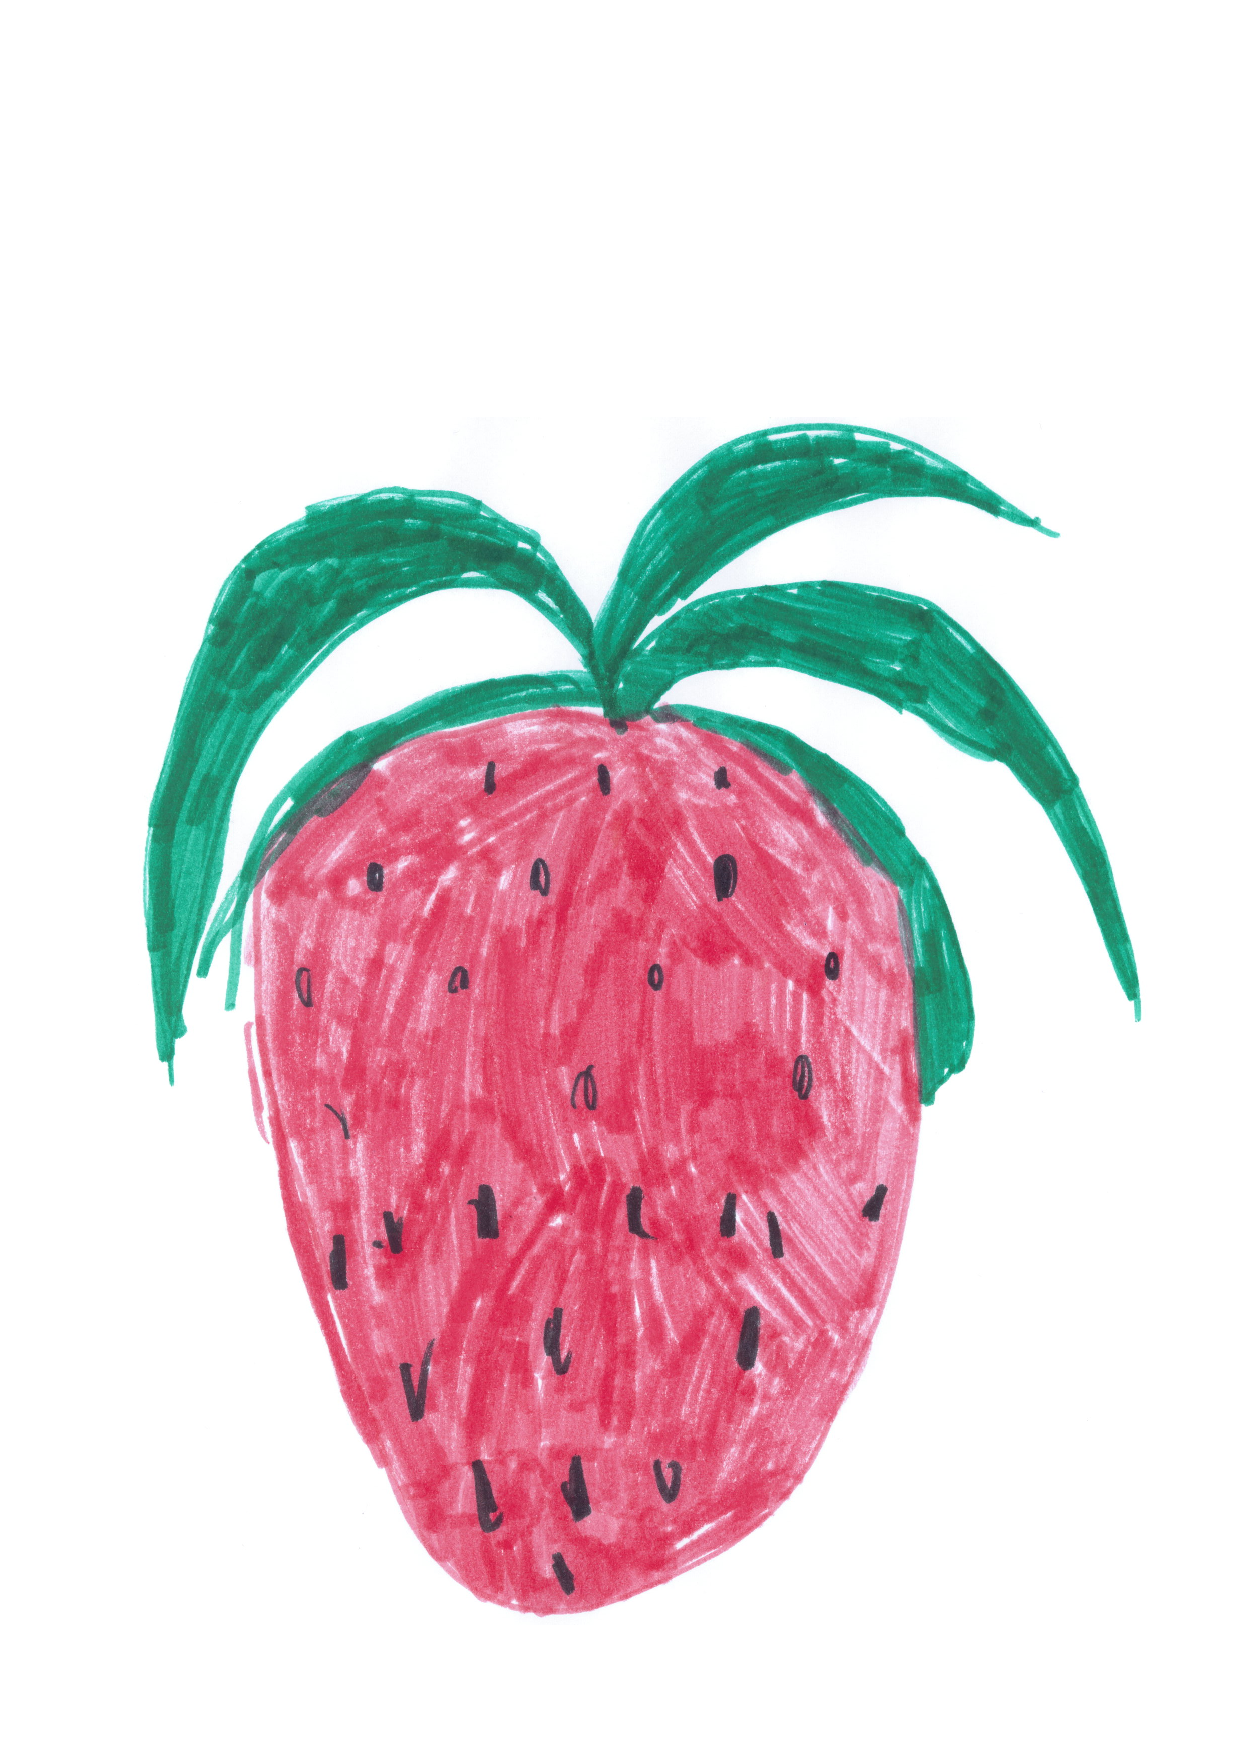
\includegraphics[width=.7\textwidth]{bilder/opa1.pdf}
\end{figure}


Die beiden liegen noch lange wach und gucken in den klaren Sternenhimmel. Sogar Glühwürmchen gibt es hier. Meret versucht eins zu fangen, das ist gar nicht so leicht. Plötzlich sieht sie ein viel grösseres Glühwürmchen mitten im Erdbeerbeet. Aber Moment, das ist ja gar kein Glühwürmchen, das leuchtet ja rot! Die Schwestern gucken erstaunt, denn was da leuchtet, ist eine Erdbeere.

Vorsichtig pflücken sie die Erdbeere. Seltsam. Mit ihrem Taschenmesser schneiden sie die Erdbeere vorsichtig auseinander. Auch innen leuchtet sie.

\enquote{Wetten, dass du dich nicht traust, so eine Hälfte zu essen.} stichelt Fenja. 

Meret ist beleidigt. Natürlich traut sie sich das. Eigentlich traut sie sich immer alles, was Fenja sagt. Das weiss Fenja und nutzt das gelegentlich aus, Meret zu Sachen anzustacheln, die ihnen eigentlich verboten sind. Oder verboten wären, wüssten Mama und Papa davon. Das kann Fenja nun mal schon besser abschätzen. Zack ist die Hälfte der Erdbeere in Merets Mund verschwunden.

\enquote{Und jetzt du die andere Hälfte.} Fenja weigert sich erst ein bisschen. Womöglich ist die Erdbeere ja schon schlecht und damit giftig. Es kommt zur üblichen Schwesterndiskussionen, die immer nach genau demselben Muster abläuft. Es geht mit dem Vorwurf \textit{Feigling} los, wird mit \textit{selber} erwidert und dann geht das wie beim Tischtennis eine Weile so hin und her. Meret ist aber diesmal klar im Vorteil, denn sie hat die eine Hälfte ja schon gegessen. Fenja muss auch, will sie nicht den Rest der Ferien das überlegene Gesicht der kleinen Schwester sehen. Das schlimmste, was passieren kann, sind Bauchschmerzen, überlegt sie. Die sind nach einem Tag aber sicher vorbei, es gibt ja schliesslich Medikamente. Also gut, und auch die zweite Hälfte ist gegessen.

Eine Weile warten beide, ob sie Bauchschmerzen bekommen, es passiert aber nichts und beim Warten schlafen sie ein.

\begin{center}
\aldineleft
\end{center}

Der nächste Morgen beginnt zunächst ganz normal. Meret hatte dann doch ein bisschen Angst bekommen, so im Zelt, deswegen war Fenja mit ihr dann doch ins Haus gegangen, um weiter zu schlafen. Opa hatte schon vorgesorgt und ein Bett vorbereitet. Mal sehen, ob es nächste Nacht klappt. Opa geht noch schnell zum Bäcker, frische Brötchen kaufen. Die beiden Schwestern sitzen draussen auf der Veranda und trinken heissen Kakao. Die Vögel zwitschern wieder, als gäbe es einen Wettbewerb, wer das wohl am lautesten kann. Die Sonne scheint auch schon wieder mit ganzer Kraft, Fenja muss blinzeln und schliesst die Augen.

\enquote{\dots und dann sagt der freche Sperling zu mir, er hätte den Wurm zuerst gesehen. Dass muss man sich einmal vorstellen. Sperlinge sind doch weiss Gott die frechsten Vögel weit und breit.}

\enquote{Ja, ja, da sagen sie ein wahres Wort, Frau Amsel, erst neulich habe ich \dots}

\begin{figure}[hb]
\centering
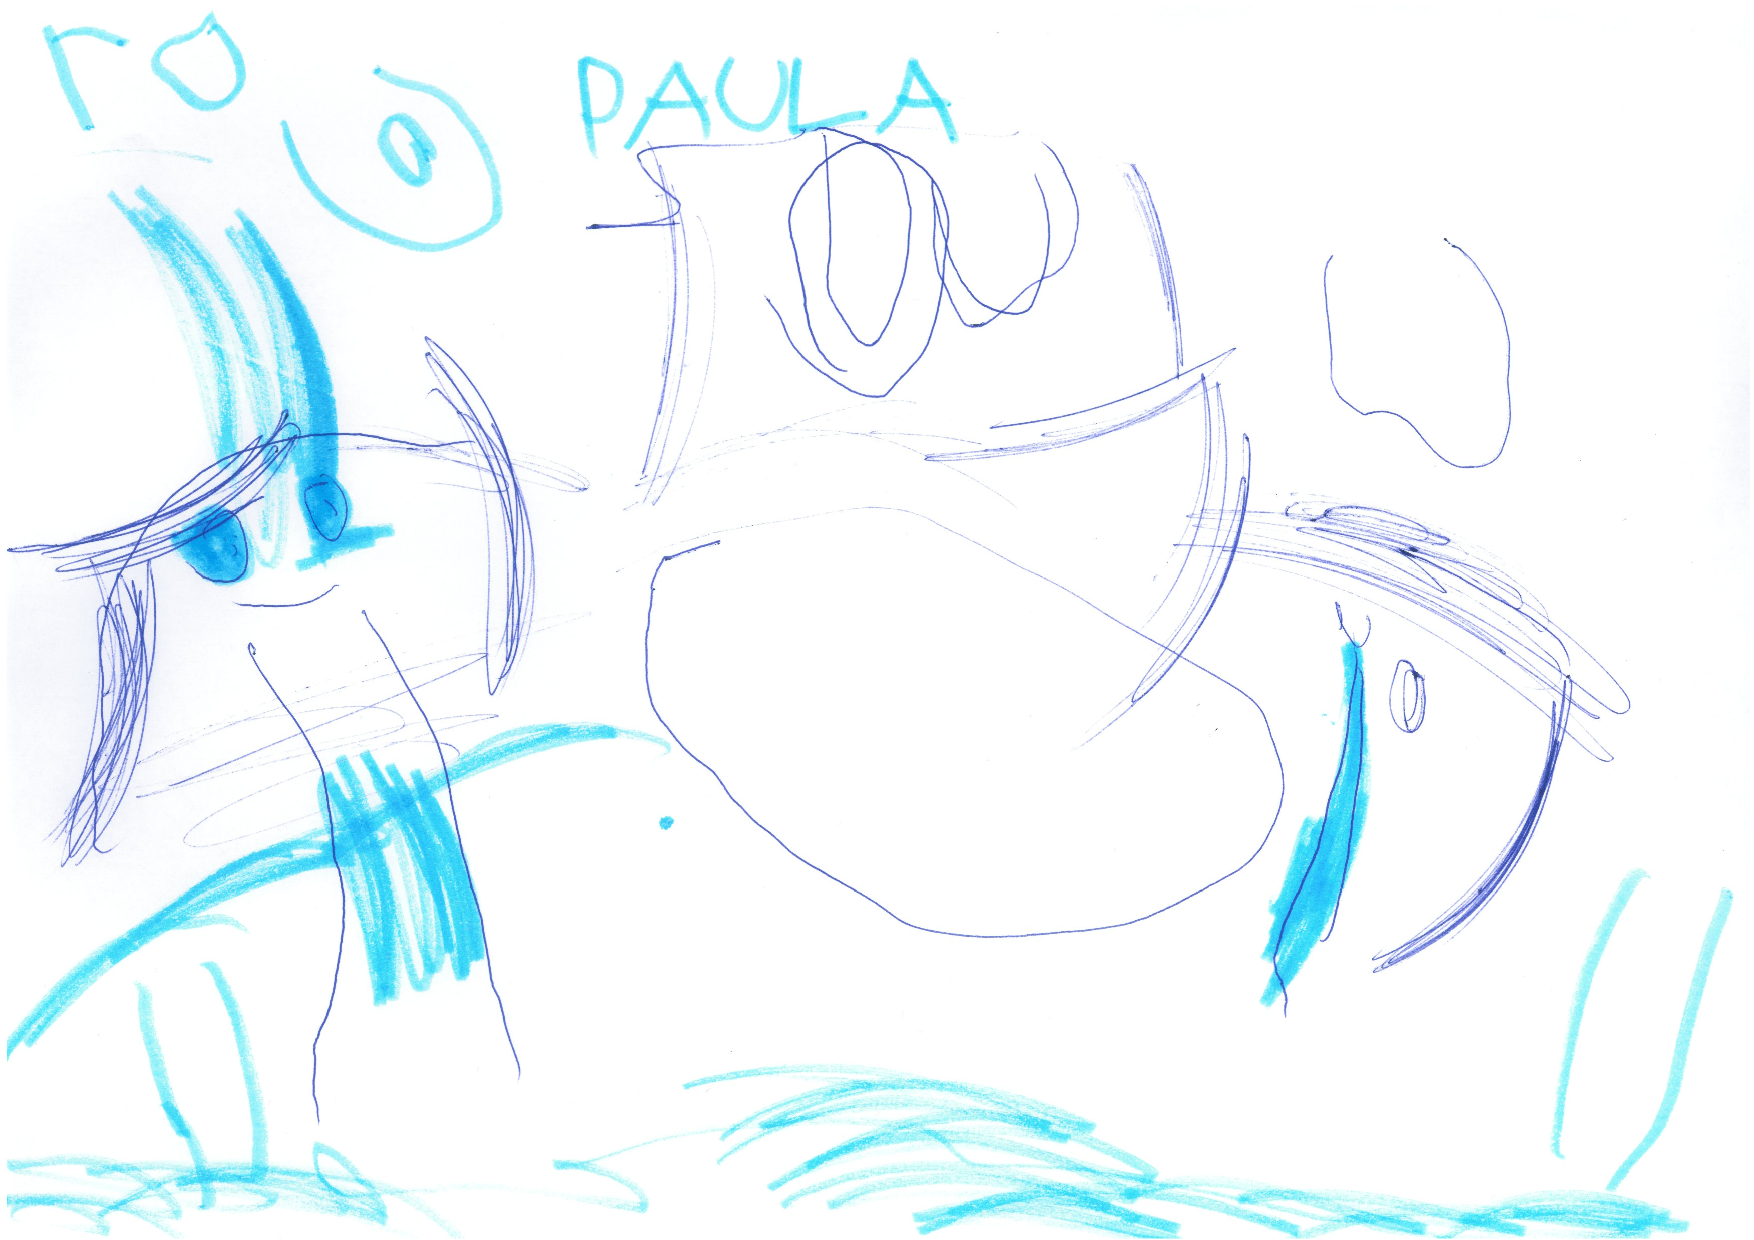
\includegraphics[width=\textwidth]{bilder/opa2.pdf}
\end{figure}

Fenja erschrickt. \enquote{Hast du das auch gehört?} fragt sie Meret. Die schlürft nur weiter an ihrem Kakao und überlegt, ob man den auch mit Erdbeeren kombinieren kann.

\enquote{Was meinst Du?}

Aber auch Fenja hört es nicht mehr. Sie konzentriert sich ganz fest, aber nichts. Um noch besser zu hören schliesst sie wieder die Augen und da sind die Stimmen wieder:

\enquote{Und überhaupt, was für ein protziges Nest sich diese Meise gebaut hat. Geschieht ihr ganz Recht, dass sie einen Kuckuck gross ziehen musst.}  

Augen wieder auf, Stimmen weg. Augen zu, Stimmen da. Auch Meret muss das ausprobieren und auch bei ihr funktioniert das. Beide sind aufgeregt. Sie verstehen die Stimmen der Vögel! Unglaublich. Sie schliessen die Augen und hören zu.

\enquote{Und haben sie gesehen meine Liebe. Die Erdbeere, die die alte Hexe gepflanzt hat ist auch weg.}

\enquote{Die Zauberbeere? Nein! Wer mag die wohl gegessen haben! Hoffentlich nicht die Hexe selber. Haben sie die übrigens gesehen in letzter Zeit?}

\enquote{Na ich glaube, die hat den Wald seit Wochen nicht mehr verlassen. Seit sie Herrn Rabe gefangen hat, habe ich nichts von ihr gehört. Wie es dem wohl geht? Vielleicht hat der Mann, der jetzt hier wohnt, die Erdbeere gegessen. Oder diese beiden jungen Mädchen, die zu Besuch sind. Schauen sie nur, da unten sitzen sie und lassen sich die Sonne auf den Bauch scheinen. Versteh einer die Menschen. Sitzen nur rum und suchen nie Futter. Also nein, also nein.}

Meret und Fenja sehen sich an. Die leuchtende Erdbeere wurde von einer Hexe gepflanzt? Was mag das für eine Hexe sein? Und warum hat sie das getan? Können sie jetzt für immer die Vögel verstehen? Tausend und eine Frage stellen sich die Schwestern gegenseitig, ohne sie beantworten zu können.

Als der Opa zurückkommt und schon von weitem mit der grossen Papiertüte mit all den frischen Brötchen winkt, ist beiden klar, dass sie erst einmal das Geheimnis für sich behalten wollen. Beim Essen fragt Fenja mit vollem Mund:

\enquote{Du, Opa, gibt es hier eine Hexe?}

\begin{figure}[hb]
\centering
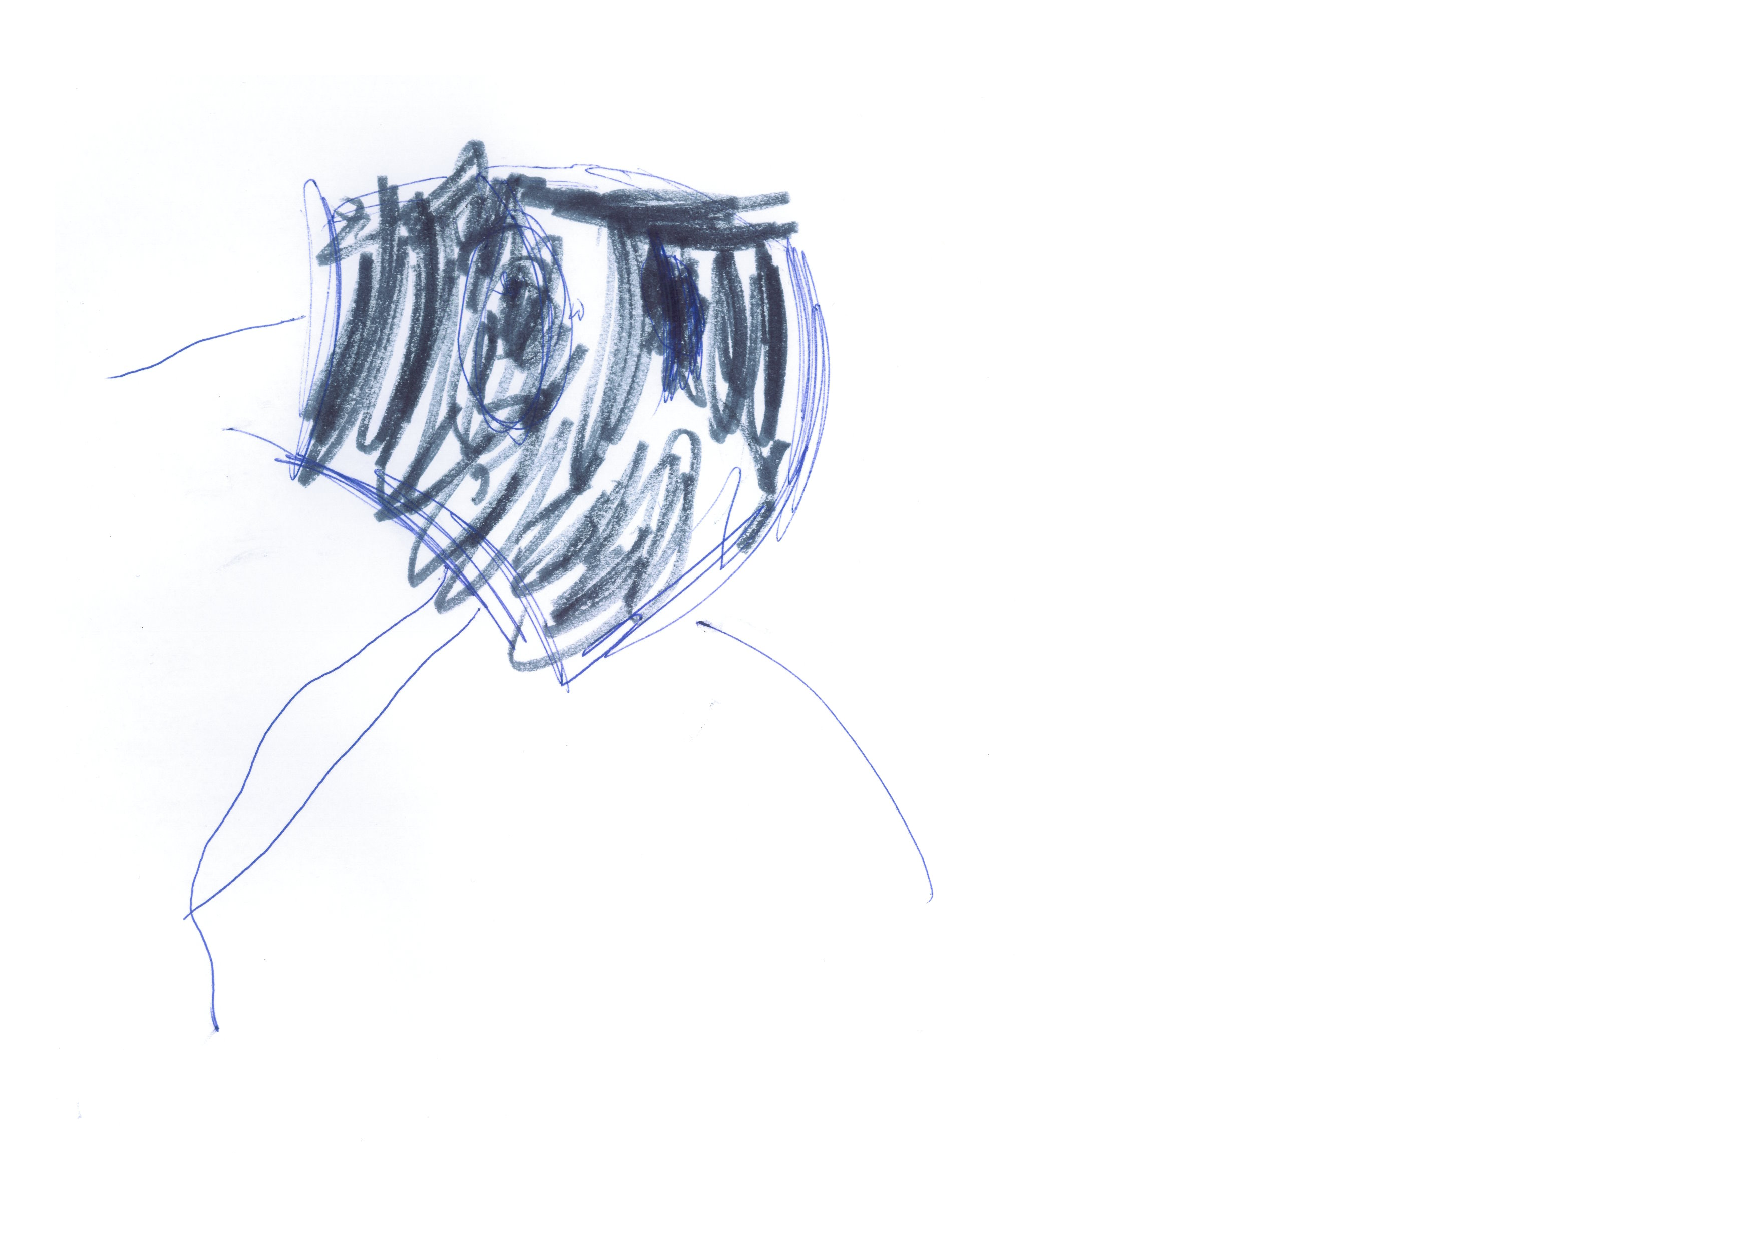
\includegraphics[width=.55\textwidth]{bilder/opa3.pdf}
\end{figure}

Opa muss lachen.

\enquote{Ihr habt mit dem Nachbarn gesprochen, stimmt's? Die alte Frau, der vorher das Haus hier gehört hat, mag zwar ein bisschen eigentümlich sein, aber eine Hexe ist sie sicher nicht. Das behaupten die Leute nur. Und das ist überhaupt nicht nett, wenn ihr mich fragt.}

\enquote{Was ist mit der Hexe -- ähm -- alten Frau jetzt?}

\enquote{Ach, die hat noch ein kleines Hüttchen oben am Waldrand. Das Haus hier war ihr zu gross, da ist sie dahin gezogen. Aber ich weiss gar nicht, ich habe sie schon lange nicht mehr gesehen. Aber wenn ihr wollt, können wir sie besuchen, ich wollte so wieso ein bisschen mit euch wandern gehen heute, da können wir ja dort vorbei.}

Die Schwestern sind einverstanden. Sie sind zwar schon ein bisschen ängstlich, immerhin wissen sie sicher, dass es eine richtige Hexe sein muss, wenn sie so Erdbeeren pflanzen kann, aber die Neugier ist einfach grösser. Noch grösser ist allerdings die Hitze, weswegen die Wanderung auf morgen vertagt wird. Heute steht erst einmal baden an. Ab in den Fluss heisst das. Nach vielen verschmutzten Jahren, ist er jetzt wieder so sauber, dass man bedenkenlos in ihm schwimmen kann.

Auf dem Weg zum Fluss kommen die drei am Wildgehege vorbei. Es gibt Wildschweine zu sehen und auch Rehe. Sogar ein weisses Reh ist dabei. Albino nennt man das, erklärt Opa, aber auch, dass das Reh sehr krank sei, keiner wisse warum.

\enquote{Der Förster sagt, dass es wohl bald sterben könnte. Da habt ihr es wenigstens nochmals gesehen.}, meint er.

Die ganze Zeit hören sie immer wieder den Vögeln zu. Unglaublich, wie viel die zu reden haben. Wer hätte gedacht, dass das viele Gezwitscher, das man immer hört, eigentlich vor allem Tratsch und Klatsch ist. Wer wo jetzt neu ein Nest gebaut hat, wird besprochen. Bei welchem Haus jetzt eine Katze wohnt. Wie schmutzig die Tauben angeblich sind und solche Dinge eben. Am schlimmsten sind die Enten. Ständig sagen sie \enquote{Guten Tag} zueinander. So als ob sie sich das erste Mal sehen. Kaum dreht sich eine Ente um und wieder zurück, schon heisst es wieder \enquote{Guten Tag, mein Herr} oder \enquote{Guten Tag, meine Dame.} Vielmehr eigentlich nicht. Manchmal noch ein paar Floskeln zum Wetter. Überhaupt sind Vögel alle immer ausgesucht höflich. Meret und Fenja ahmen das die ganze Zeit nach, was den Opa dann doch ein wenig verwundert.

\begin{center}
\aldineleft
\end{center}

Obwohl es am nächsten Morgen schon wieder so heiss ist, wollen die beiden Schwestern trotzdem unbedingt zu der alten Frau. Opa winkt ab.

\enquote{Nein meine Lieben, geht ihr gerne alleine, mir ist es zu heiss zum Wandern.} Es wird noch kurz erklärt, wo es lang geht, und dann los.

Beide Mädchen sind schon etwas aufgeregt und ängstlich.

\enquote{Und was ist, wenn sie uns wie bei Hänsel und Gretel\dots?} fängt Meret an zu fragen, wird aber von ihrer Schwester unterbrochen.

\enquote{Paperlapapp.} Sie kann zwar auch nicht sagen, auf was sie sich einlässt, aber ihr Gefühl sagt ihr, dass es schon nicht wirklich gefährlich werden kann. Sie erreichen den Wald, der hier sehr wild und dicht ist. Nach der vielen Sonne auf den Wiesen auf dem Weg, wirkt der Wald richtig düster, aber eigentlich nicht bedrohlich.

Als die Hexe dann völlig unerwartet neben ihnen steht, sind beide sehr erschrocken. In der Hand hält sie einen Bund irgendwelcher Kräuter und trägt eine schmutzige braune Kittelschürze.

\enquote{Was machen denn zwei so hübsche junge Mädchen bei dem Wetter hier im Wald. Ihr seid ja gar nicht baden?}

Keine der Schwestern weiss etwas zu sagen.

Fenja hat mehr Mut und denkt sich, wenn das wirklich eine Hexe ist, sollte man vielleicht nichts verheimlichen. Eine echte Hexe merkt bestimmt, wenn man schwindelt.

\enquote{Unser Opa ist der Mann, der ihr Haus gekauft hat. Und er hat uns gesagt, wo sie wohnen und da dachten wir, dass wir sie vielleicht einmal besuchen sollten.}

Die Alte brummt etwas vor sich hin, dann stutzt sie, überlegt und mustert die beiden von oben bis unten.

\enquote{Eine von Euch hat die Erdbeere gegessen, richtig? Und jetzt könnt ihr die Vögel verstehen. Ja, die Erdbeere hatte ich ganz vergessen, das passiert im Alter.}

\enquote{Beide.} geben die Schwestern zu, denn irgendwie haben sie nicht das Gefühl, dass die Frau böse ist. 

\enquote{Na was sagen sie denn, die Vögel? Hört es euch gut an, spätestens beim nächsten Vollmond, also heute Nacht, ist das wieder vorbei. Aber es wird auch wieder eine neue leuchtende Erdbeere wachsen, nächste Woche oder übernächste.} 

Die beiden erzählen, was sie so gehört haben, auch, dass sie, die Hexe, einen Raben gefangen haben soll. Die Hexe lacht und sagt, sie sollen mal mitkommen, sie können ja selber hören, was der Rabe zu erzählen hat. Und so gelangen sie zu dem Haus, in dem die Hexe wohnt. Ein einfaches Hüttchen, eine Art Gartenhäuschen. Hier ist es bestimmt ziemlich kalt im Winter, denkt Fenja. 

Der Rabe sitzt auf dem Rahmen einer Hollywood-Schaukel und hat einen Verband um den linken Flügel. Die Mädchen schlissen die Augen und hören den Raben sagen, dass er sich den Flügel gebrochen hat, den er aber lustigerweise Arm nennt und das die Hexe ihm geholfen haben.

Beide sind beruhigt und kein bisschen ängstlich mehr. Es gibt kalten Kräutertee, der sehr gut schmeckt. 

\enquote{Und haben die Vögel ein weisses Reh erwähnt? Deswegen habe ich die Erdbeeren damals überhaupt nur gepflanzt. Ich spüre, dass es diesem Reh nicht gut geht, es ist krank und es ist irgendwo eingesperrt oder gefangen. Und ich dachte, wenn ich den Vögeln zuhören kann, die aus der Luft ja alles sehen, erfahre ich vielleicht, wo das Reh ist, damit ich ihm helfen kann. Es hat Probleme mit dem Herz und ich habe die Kräuter, die ihm helfen. Leider kann man ja die Vögel nicht fragen, sondern nur hören, was sie sagen und wie ihr selber gemerkt habt, reden die Vögel meist nur Unsinniges, da habe ich das irgendwann aufgegeben.}

Die beiden Schwestern sind aufgeregt. Sie wissen natürlich, wo das weisse Reh ist. Im Wildgehege! Sie haben es ja selbst gestern erst gesehen! Die Hexe klatscht vor Freude in die Hände. 

\enquote{Wer hätte gedacht, dass ich es doch noch mit Hilfe der Erdbeeren finde!} Sie geht ins Haus und kommt mit einem Säckchen voller Kräuter zurück. 

\enquote{So ihr beiden. Seid so nett und helft mir, wir gehen gleich los.} Mit diesen Worten stellt sie einen alten Stuhl auf einen Bollerwagen mit einem energischen Blick, der keinen Zweifel daran lässt, dass die beiden Schwestern sie ziehen sollen. Kein Problem für die beiden. Es wird \textit{Das Wandern ist des Müllers Lust} und \textit{Hab mein Wagen voll geladen} gesungen und so vergeht die Zeit sehr schnell, bis sie beim Tiergehege sind.

Die Hexe streckt die Hand aus und alle Rehe kommen angelaufen. Auch das weisse.

\enquote{Da bist du ja, haben sie dich hier eingesperrt, deswegen habe ich dich nicht gefunden.} sagt sie und hält ihm ihre Kräuter hin, die es auch frisst.

Sie begleiten die Hexe wieder nach Hause und versprechen, sie nochmals besuchen zu kommen, so lange sie noch beim Opa sind. Beide Schwestern sind erleichtert, dass die Vögel auch mit geschlossenen Augen wieder zwitschern. Der Zauber der leuchtenden Erdbeere ist wieder verschwunden.

Am Abend gibt es schon wieder Bratwürste und rosa Erdbeermilch. Während Opa die Bratwürste dreht, sind die Vögel nochmals besonders laut.

\enquote{Was die wohl zu erzählen haben?} meint er. \enquote{bestimmt erzählen die sich die verrücktesten Geschichten.}

Meret und Fenja müssen lachen und sagen wie aus einem Mund:

\enquote{Na da wäre ich mir nicht so sicher, Opa.} \hfill {\color{red}\decofourleft}


\chapter*{\FontH{\Huge Das schwarze Licht}}
\addcontentsline{toc}{chapter}{Das schwarze Licht}
\lettrine[lines=3]{\color{red}D}{}\begin{swb}as Dorf Ragunda lag tief in schwedischen Wäldern, da, wo es noch Trolle und Feen und andere Wesen gab, die es sonst nur noch in Geschichten gibt. Das war ein Glück für die Menschen, denn gerade die Trolle waren eine grosse Hilfe, denn sie hatten sehr viel Kraft. Musste eine Brücke gebaut werden, war immer ein Troll in der Nähe, der gerne half. Aber es gab auch Wesen in diesen Wäldern, die gefährlich sein konnten. Gelegentlich wütete ein Thurse, das ist ein besonders grosser Riese. Aber zwei oder drei Trolle genügten meist, ihn in die Wälder zurück zu jagen, bevor er grossen Schaden anrichten konnten. Ganz selten aber suchte den Wald um Ragunda aber ein Wesen heim, dass viel gefährlicher und mächtiger war, als Trolle und Thursen, nämlich ein Guhl. Schon lange war keiner mehr gesehen worden, nur ein alter Mann konnte sich erinnern, dass der Grossvater seines Grossvaters einmal einen erlebt hatte. Und die Geschichten vom Guhl, die er wusste, erzählte er abends den Kindern, denen es zwar Spass machte, sich zu gruseln, aber die dem alten Mann auch nicht recht glauben wollten. 

Er erzählte dann, das es gut sei, dass so ein Guhl sehr lange schläft, nämlich oft über tausend Jahre, verborgen in einer Höhle tief unter der Erde. Wenn er aber aufwacht, können die schrecklichsten Dinge passieren. Manch ein Guhl kann die Erde erzittern lassen, so dass die Häuser einstürzen oder den Wald mit seinem heissen Atem in Brand setzen. Guhle, die am Meer leben können fürchterliche Überschwemmungen bringen, die alles mit einer riesigen Welle wegspült. Aber nur selten passiert so etwas, denn selbst wenn ein Guhl wach ist, ist er eigentlich nur gefährlich, wenn er wütend ist und das sind Guhle selten.

Krokusse und Adonisröschen gaben dem Wald gerade die ersten Farbtupfer nach einem strengen  und langen Winter als ein Kurier aus dem Nachbardorf in Ragunda eintraf und die schreckliche Nachricht überbrachte. Ein Guhl war aus seinem Schlaf erwacht. Ein unvorsichtiger Jäger hatte seinen Pfeil versehentlich in die Höhle des Guhl geschossen und ihn damit geweckt.

\begin{figure}[hb]
\centering
\includegraphics[width=.7\textwidth]{bilder/dark.pdf}
\end{figure}

\begin{figure}[hb]
\centering
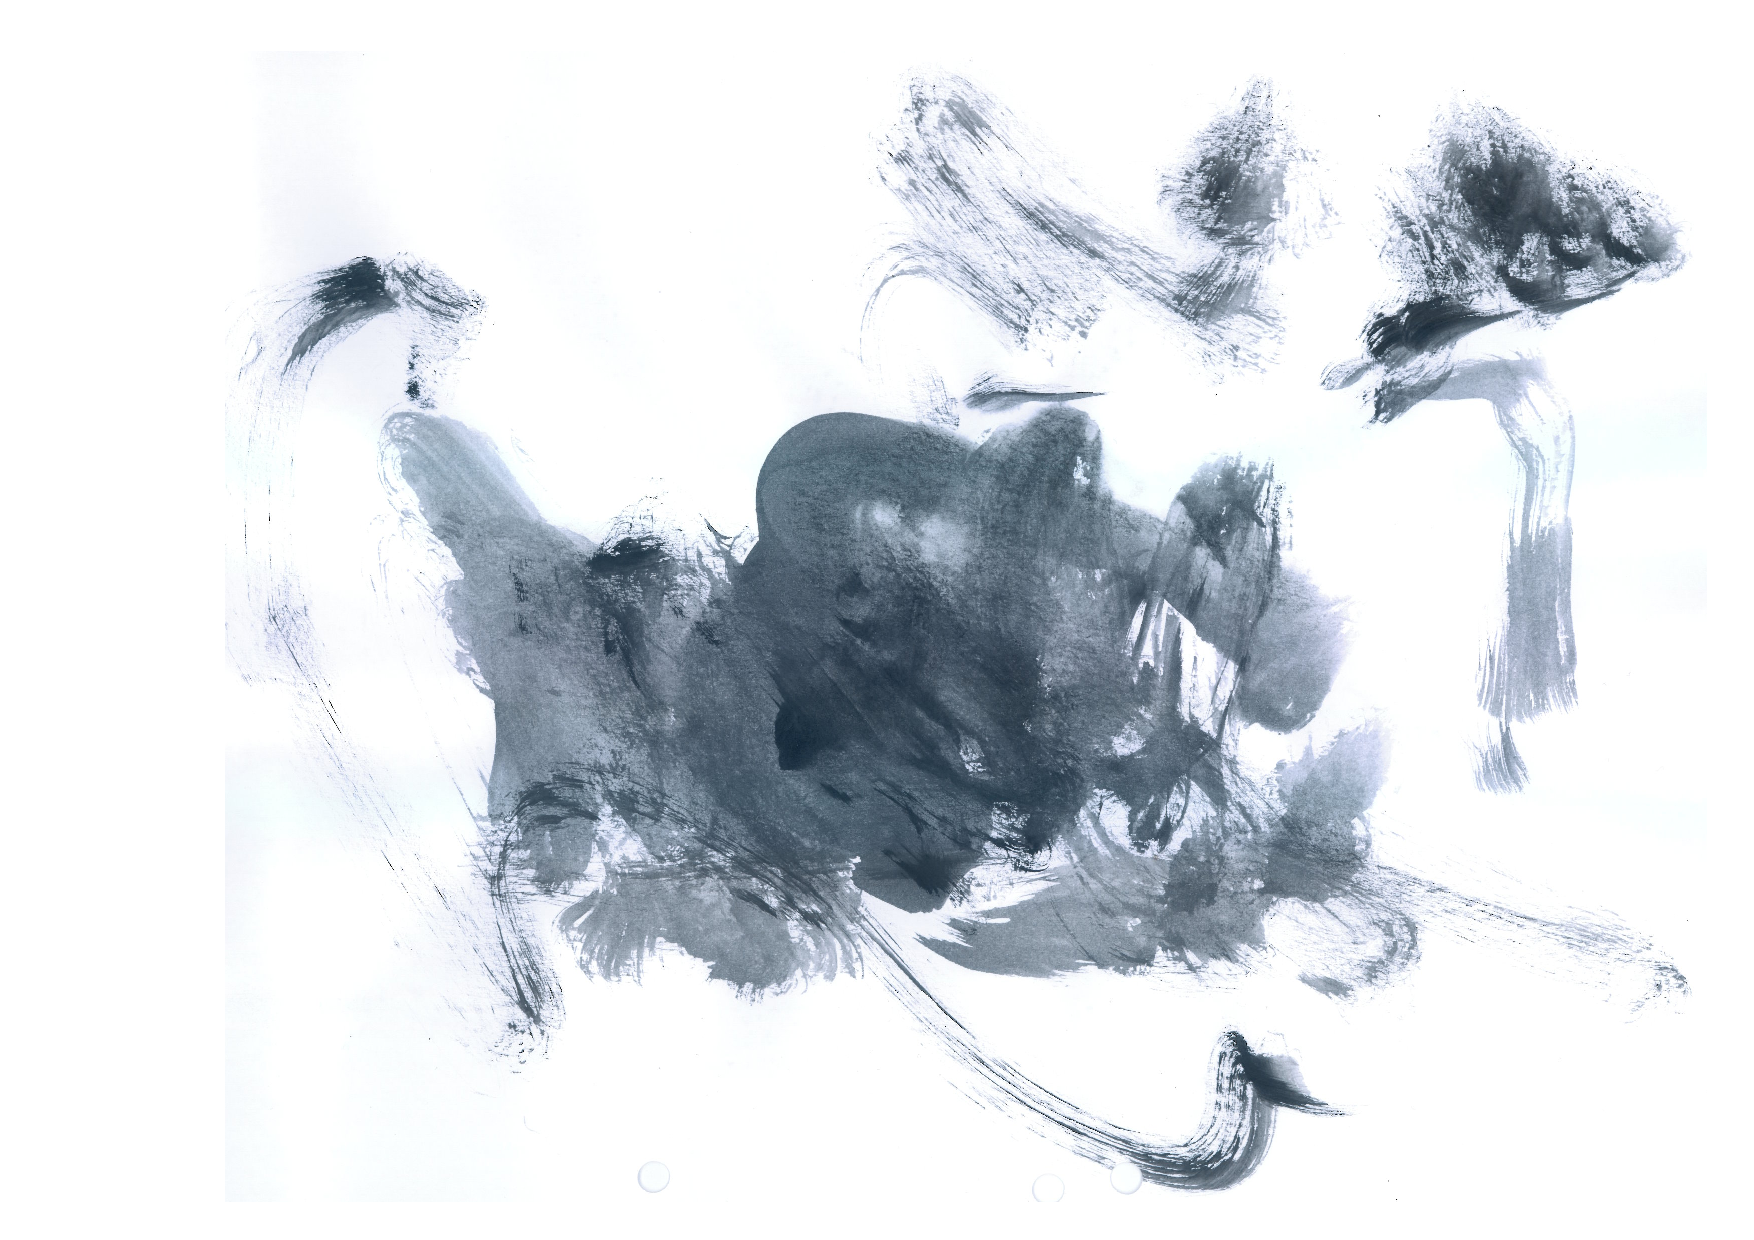
\includegraphics[width=.7\textwidth]{bilder/dark2.pdf}
\end{figure}

Der Guhl, der geweckt worden war, hatte eine ganz besonders gefährliche Fähigkeit, er konnte schwarzes Licht ausstrahlen. Es gibt nichts dunkleres auf dieser Welt, als schwarzes Licht. Man kann es nicht bekämpfen. Das schwarze Licht eines Guhl frisst alles Helle. Egal wie gross das Feuer ist, dass man anzündet, das schwarze Licht des Guhls ist stärker. Auch die Sonne ist nicht stark genug, es zu durchbrechen. Wo das schwarze Licht ist, herrscht tiefste Dunkelheit, viel dunkler als in der schwärzesten Nacht, wenn man im Keller sitzt, die Augen schliesst und noch eine Decke über den Kopf gelegt hat. Das schwarze Licht kann alles durchdringen und wo es ist, können die Pflanzen nicht mehr wachsen und die Tiere fliehen oder sterben. Viele Wüsten sind einmal entstanden, weil ein Guhl mit seinem schwarzen Licht gewütet hat. 

Und wenn das schwarze Licht die Menschen erreicht, ist es meist um sie geschehen. Die Felder verdorren und das Vieh stirbt, so dass sie nichts mehr zu Essen haben. Aber das schwarze Licht umschliesst auch die Menschen. In völliger Dunkelheit fangen sie auch am tage an zu träumen und können die träume nicht mehr von der Wirklichkeit unterscheiden. Furchtbare Albträume schütteln sie und alle leben in ständiger Angst.


Die Menschen in Ragunda wussten oder ahnten das. Der Bote hatte gesagt, dass grosse Teile des Waldes schon fest im Griff des schwarzen Lichtes seien. In Ragunda brach Panik aus, Die Bewohner packten ihre Sachen und wollten fliehen, denn wo das schwarze Licht ist, gibt es schon bald keine Nahrung mehr. Aber noch bevor sie sich einigen konnten, in welche Richtung sie fliehen sollten, war plötzlich alles schwarz. Es ging viel schneller, als sie dachten. Kinder fingen an zu weinen und die Erwachsenen wussten nicht, was sie jetzt tun sollten. Schwärze legte sich über das Dorf und kroch durch jede Ritze. Zündete man eine Kerze an, verbrannte man sich nur die Hände, denn auch die Flamme war schwarz. Mühsam tasteten sich die Menschen durch ihre Häuser auf der Suche nach Essen. Aber die Vorräte waren nach dem Winter aufgebraucht und etwas neues wuchs nicht.

Und mit der Dunkelheit kamen die Albträume. Schnell machte sich grosse Angst breit und die Menschen verbarrikadieren sich in ihren Wohnungen. 

In all dem Chaos und der Angst hatte nur ein Mädchen keine Angst: Onta. Onta war schon blind geboren worden, ihre fehlte das Licht also nicht. Sie wusste genau wie viele Schritte es vom Tisch bis zur Tür und von dort bis überall hin im Dorf sind. Sie konnte sogar im Wald rennen, so genau hatte sie sich eingeprägt, wo welcher Baum stand. Es dauerte ein paar Tage, bis ihr klar wurde, dass nur sie jetzt noch helfen kann.

Und so machte sich Onta auf den Weg, den Guhl zu suchen, um ihn zu besänftigen. Wie das gelingen könnte, wusste sie selbst noch nicht so genau. 

Noch nie hatte sie den Wald so leise erlebt. Um so weiter sie kam, um so vorsichtiger musste sie sich den Weg ertasten. Aber sie wusste, dass sie auf dem richtigen Weg war, denn der Gestank des Guhl wurde von Stunde zu Stunde stärker. Nach ungefähr einem Tag Wanderung war sie sicher am Ziel zu sein. Der Guhl musste jetzt ganz in der Nähe sein.

Onta setzte sich auf einen Stein und wartete. Um sich die Zeit zu vertrieben und gegen die Angst und die Stille nahm sie ihre kleine geschnitzte Flöte und spielte ein Lied. Plötzlich stand der Guhl hinter ihr. Onta konnte ihn spüren. Er musste riesig sein. Niemand wusste genau, wie so ein Guhl aussieht, vielleicht ein bisschen wie ein riesiger Bär. Jedenfalls brummte er wie einer, blos sehr viel lauter. Aber Onta merkte, dass nichts Böses in diesem Brummen lag. 

Den Geräuschen nach hatte sich der Guhl auf den Boden gesetzt. Onta spielte einfach weiter und immer weiter. Das Brummen des Guhl war immer gleichmässiger geworden und einem Schnarchen gewichen. Der Guhl war wieder eingeschlafen. Onta spielte weiter so lange sie konnte. Es könnte ein Tag gewesen sein oder zwei, als sie das leise Knacken von Zweigen hinter sich hörte.

Mit ganz leiser Stimme flüsterte eine Stimme ihren Namen. Da hörte Onta auf zu spielen, der Guhl schlief weiter. Die Stimme gehörte einer Jägerin des Dorfes, die sie suchen gekommen war. Als der Guhl eingeschlafen war, war auch das schwarze Licht verschwunden. Onta hatte dies noch nicht bemerkt, da bis hier noch keine Vögel zurückgekehrt waren.

Die Menschen des Dorfes bauten eine grosse Mauer um den Guhl. Nicht um ihn einzusperren, das wäre unmöglich gewesen, sondern um seinen Schlaf zu schützen.  \end{swb}\hfill {\color{red}\decofourleft}

\mdfsetup{
%
frametitle={
%
\tikz[baseline=(current bounding box.east),
outer sep =0pt]
\node[anchor=east,rectangle,fill=red]
{\color{white} \small Nina \& Oma Lena};},
frametitleaboveskip=\dimexpr-\ht\strutbox\relax
}
\pagenumbering{gobble}
\pagestyle{empty}
\section*{\FontH{\Huge Der Fall der verschwundenen Schmetterlinge}}
\centerline{\Huge \color{red}\SixFlowerPetalDotted}
\vspace{13pt}
\centerline{\bf \large\color{red}Für Papapa zum Geburtstag }
\vspace{13pt}
\centerline{\bf \color{red} von Linda, Paula, Doris und Gordon}
\vspace{13pt}
\centerline{\huge \color{red}\SixFlowerPetalDotted}
\vspace{13pt}
\centerline{\LARGE \color{red}\SixFlowerPetalDotted}
\vspace{13pt}
\centerline{\Large \color{red}\SixFlowerPetalDotted}
\vspace{13pt}
\centerline{\large \color{red}\SixFlowerPetalDotted}
\vspace{13pt}
\centerline{\normalsize \color{red}\SixFlowerPetalDotted}
\vspace{13pt}
\centerline{\small \color{red}\SixFlowerPetalDotted}
\vspace{13pt}
\centerline{\footnotesize \color{red}\SixFlowerPetalDotted}
\vspace{13pt}
\centerline{\scriptsize \color{red}\SixFlowerPetalDotted}
\vspace{13pt}
\centerline{\tiny \color{red}\SixFlowerPetalDotted}

\newpage
\pagestyle{scrheadings}
\pagenumbering{arabic}

\lettrine[lines=3]{\color{red}D}{as} Mobiltelefon klingelt und weckt Fenja aus dem Schlaf. Es ist noch sehr früh am Morgen. Zuerst bemerkt Fenja, dass es noch gar nicht hell ist. Eine Frechheit, wer ruft sie so früh an? Am Klingelton erkennt sie sofort, dass es Kommissarin Bettina Andermatt sein muss. Die Melodie vom rosaroten Panther.

Sofort ist sie hellwach. Fenja geht zwar noch in die Schule, aber sie ist sehr intelligent und kann sehr gut beobachten. Ihr fällt alles auf. Und sie vergisst nie, wann etwas passiert ist, egal wie lang das schon zurück liegt. Ihre Mutter sagt, das hätte sie von Papapa geerbt, als ob immer alles irgendwoher geerbt werden müsste. Aber in dieses Mal hat sie wohl Recht. 

Der Polizei ist es egal, wo das Talent jetzt genau herkommt, weiss es aber sehr zu schätzen und bittet sie regelmässig bei besonders verzwickten Fällen, bei der Aufklärung zu helfen. Es scheint wieder einmal soweit zu sein.

\enquote{Ja, aha, ich verstehe.} Fenja schreibt alles, was die Kommissarin sagt, in ein kleines Notizbuch, dass immer auf ihrem Nachtschränkchen liegt. Im Papiliorama in Kerzers sind Schmetterlinge verschwunden. Seltene, besonders schöne Exemplare der Gattungen \emph{Morpho peleides}.

\enquote{Entschuldigen sie die Frage, Frau Kommissarin, aber könnte es sein, dass die Schmetterlinge einfach abgehauen sind? Ich selbst würde auch jede Gelegenheit nutzen, wenn ich so eingesperrt wäre.} Im Zimmer kann man hören, wie die Kommissarin am anderen Ende der Leitung lauter wird. Für vorlaute Spässe habe sie keinen Sinn, schon gar nicht um diese Uhrzeit, hört man sie fast brüllen. Sie erklärt, dass es auffällig ist, dass nur Schmetterlinge eben jener Sorte verschwunden sind. Ausserdem sind auch alle Raupen weg.

Fenja verspricht der Sache sofort am nächsten Morgen nachzugehen und legt auf. Zunächst müssen die organisatorischen Dinge geklärt werden. Das Papiliorama liegt in Kerzers, das weiss Fenja aber schon. Erst neulich ist sie mit den Grosseltern dort gewesen. Das ist ein schöner Ausflug gewesen. Der erste Zug geht 7:32\,Uhr. Jetzt ist es 4:35\,Uhr. Genügend Zeit, sich vorzubereiten. Folgende Dinge kann Fenja mit Hilfe des Internet bereits recherchieren:

\begin{description}
	\item[Morpho peleides] \sffamily{Deutsch: Blauer Morphofalter. Der Schmetterling gehört zur Familie der Edelfalter. Die Flügel haben blaue Oberseiten und können eine Spannweite bis 12\,cm haben. Sie ernähren sich von faulenden Früchten.}
\end{description}

Fenja staunt. So riesige Schmetterlinge hat sie noch nie gesehen. Mit Hilfe des Lineals macht sie in ihrem Notitzheft ein Quadrat mit einer Höhe und Breite von je zwölf Zentimetern und zeichnet einen Schmetterling. Den malt sie blau aus. 

Dann beginnt sie ihren Rucksack zu packen. Sie benötigt:

\begin{enumerate}
  \item Die Detektivausrüstung bestehend aus ein paar sauberen Handschuhen, einer Lupe, einer Pinzette und ein paar leeren kleinen Tüten. Dazu ganz wichtig, gelbe Schnur vom Papapa.
  \item Orangensaft und Käsebrot. Aber ohne Tomaten, wie das Papa immer macht, da wird der Käse immer ganz weiss und das findet Fenja ekelig.
  \item Regenjacke, Mütze und Gummistiefel, erfahrungsgemäss finden Verbrecherjagden auch bei Schlechtwetter statt.
  \item Etwas Geld. Damit kann man dann so einiges kaufen, je nachdem, was gebraucht wird. Einmal war es nötig, sofort eine aufblasbare Kuh zu kaufen. Ein sehr merkwürdiger Fall war das damals.
  \item Einen Fotoapparat, um Tatorte dokumentieren zu können. Ein furchtbares Gerät. Es hatte lange gedauert, bis sie gemerkt hatte, dass man beim Bilderbetrachten drücken muss und nicht drehen darf. Grosi hatte es ihr dann gezeigt.
\end{enumerate}

Das alles passt wunderbar in ihren Rucksack. Noch die Schuhe und dann\dots steht plötzlich Carla vor ihr, das ist ihre kleine Schwester. Die wacht immer sehr früh auf und scheint etwas bemerkt zu haben. Carla ist zwar noch ziemlich klein, aber auch nicht dumm. Sofort begreift sie, dass Fenja etwas vor hat. Und sie weiss genau, dass es mit ihrer grossen Schwester immer aufregende Dinge zu erleben gibt.

\enquote{Wenn Du mich nicht verrätst, was du vor hast, fange ich so laut an zu weinen, dass Mama und Papa aufstehen.}

Das hätte gerade noch gefehlt. Die wollen nämlich eigentlich nicht, dass Fenja der Polizei hilft. Viel zu gefährlich meinen sie. Lächerlich. 

\enquote{Was willst du?} fragt Fenja. \enquote{Wenn Du leise bist, erlaube ich Dir so viele Trickfilme auf meinem Computer zu sehen, wie du willst.} Das ist zwar tatsächlich das verführerischste Angebot, dass die grosse Schwester machen kann, aber Carla lässt sich nicht beirren. Fenja seufzt. Ihr bleibt nichts anderes übrig, als Carla alles zu erklären und nach einer kurzen, aber überzeugenden Diskussion auch mitzunehmen. 

Aber das ist gar nicht so schlimm, überlegt Fenja. Eine kleine Schwester ist die beste Tarnung.   Jetzt in den Ferien sind viele Kinder im Papiliorama, da fallen sie beide gar nicht auf und können sich in Ruhe umsehen.

\begin{center}
\aldineleft
\end{center}
%\vspace{10pt}
% \centerline{\Huge \Dolphin[red]}
%\vspace{10pt}

Der Zug erreicht Kerzers pünktlich. Auf dem Weg zum Papiliorama schärft Fenja ihrer Schwester ein, dass sie nicht zum Spass hier sind. Die Schmetterlinge kann man sich auch ein anderes Mal wieder ansehen. Jetzt heisst es ermitteln und Spuren sammeln.

Der Direktor des Papilioramas, Herr Butterblom, weiss, dass Fenja kommen wird. Kommissarin Andermatt hat ihn schon informiert. Fenja entscheidet, dass es das beste ist, sich erst einmal in Ruhe umzusehen, um einen Eindruck vom Tatort zu bekommen. Die beiden Schwestern wollen getrennt ins Papiliorama gehen und sich in einer Stunde in der Cafeteria bei den Süssigkeiten treffen. Niemand wird glauben, dass Carla auch ermittelt.

Fenja hat sich überlegt, dass es sich bei den Dieben der Schmetterlinge nur Menschen handeln kann, die sich auf irgendeine Art für Schmetterlinge interessieren. Denn wertvoll sind sie nicht.  

\enquote{Herr Butterblom, wer könnte ein Interesse an diesen Schmetterlingen haben?} Fenja weiss, welche Fragen als erstes gestellt werden müssen. Herr Butterblom überlegt.

\enquote{Das weiss ich auch nicht. Es gibt natürlich Leute, die sich für Schmetterlinge interessieren und die selber züchten. Und da kommt es schon einmal vor, dass die hier ein paar Raupen klauen. Aber gleich alle? So etwas ist noch nie passiert.} 

\enquote{Kennen sie diese Sammler? Können sie mir vielleicht die Liste aller Namen geben?} will Fenja wissen.

\enquote{Natürlich nicht.} antwortet Herr Butterblom. Was für eine Frage. Jetzt kommen ihm doch Zweifel, ob es geschickt von Kommissarin Andermatt war, ein Kind zu schicken. Woher soll er denn die Namen der Leute kennen, die Schmetterlinge züchten? Aber Fenja ist etwas schlauer als er.

\enquote{Auf ihrer Web-Seite habe ich gesehen, dass sie auch Tagungen zu Schmetterlingen organisieren. Beispielsweise hat gerade letzte Woche jemand von der Universität einen Vortrag zu Schmetterlingen in den Alpen gehalten.} Fenja ist wirklich sehr gut vorbereitet. 

\enquote{Ich denke, dass alle, die sich für Schmetterlinge interessieren, auch an solchen Veranstaltungen teilnehmen. Es wäre sehr hilfreich, wenn sie mir die Anmeldelisten der letzten beide Jahre per E-Mail schicken könnten.}

Herr Butterblom ist verblüfft. Tatsächlich. Wenn es Züchter gibt, dann kommen die auch hierher und bei Veranstaltungen muss man immer vorher seinen Namen nennen, damit man reservieren kann. 
\begin{center}
\aldineleft
\end{center}

Zur selben Zeit schlendert Carla durch die Gänge des Papilioramas. Es ist gerade eine Sonderausstellung zum Thema \emph{Schmetterlinge in der Kunst}. Künstlerinnen und Künstler aus der Umgebung wurden eingeladen, ihre Sicht auf Schmetterlingen zu zeigen. Jemand hat einen grossen Schmetterling aus Stahl geschweisst, das ist das auffälligste Ausstellungsstück. Daneben gibt es ein paar Bilder an der Wand und eine Designerin hat sogar Kleidungsstücke mit Schmetterlingen bedruckt. Carla fotografiert alles sorgfältig mit der Kamera von Fenja.

\enquote{Alles grosser Unfug! Ganz schreckliches Zeug.} hört Carla neben sich sagen. Eine gross gewachsene Frau mit einem sehr eigenartigen Hut blickt verächtlich auf die ausgestellten Dinge. Carla fragt:

\begin{figure}[hb]
\centering
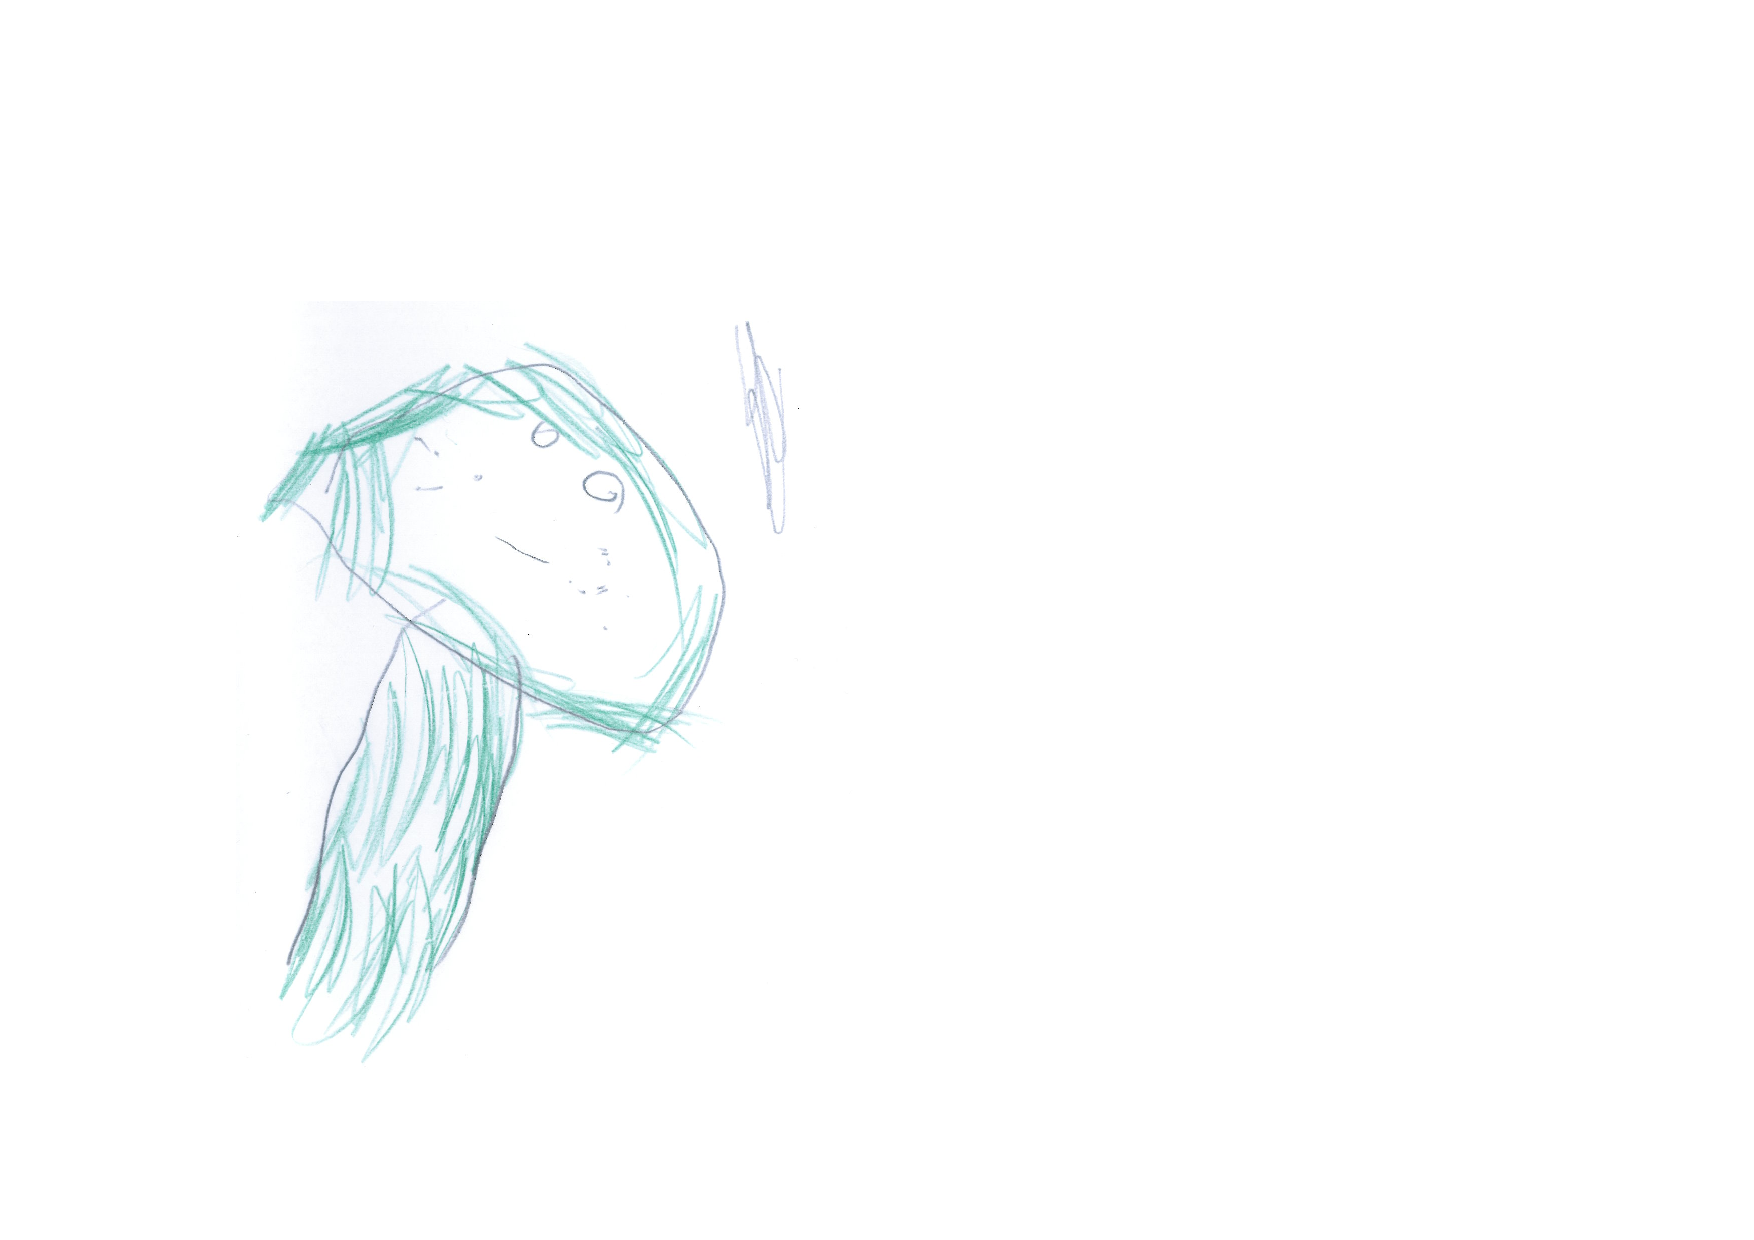
\includegraphics[width=.5\textwidth]{bilder/schmetterlingg.pdf}
\end{figure}

\enquote{Ihnen gefallen die Bilder wohl nicht besonders?}

\enquote{Natürlich nicht.} ruft die Frau mit sich überschlagender Stimme. \enquote{Das ist doch alles Unfug. Neben der Schönheit der Farben eines echten Schmetterlings, ist das hier alles blass und langweilig.} Und dann ergänzt sie:

\enquote{Darf ich mich übrigens vorstellen? Mein Name ist Verena Studer-Matt und das Kleid dahinten} dabei deutet sie auf die schmetterlingsgemusterten Kleider \enquote{sind übrigens von mir entworfen. Aber auch die finde ich mittlerweile ganz grauenvoll. Wer einmal die Schönheit eines Blauen Morphos gesehen hat, ist für derartiges verloren.} 

%\begin{figure}[h]
%\centering
%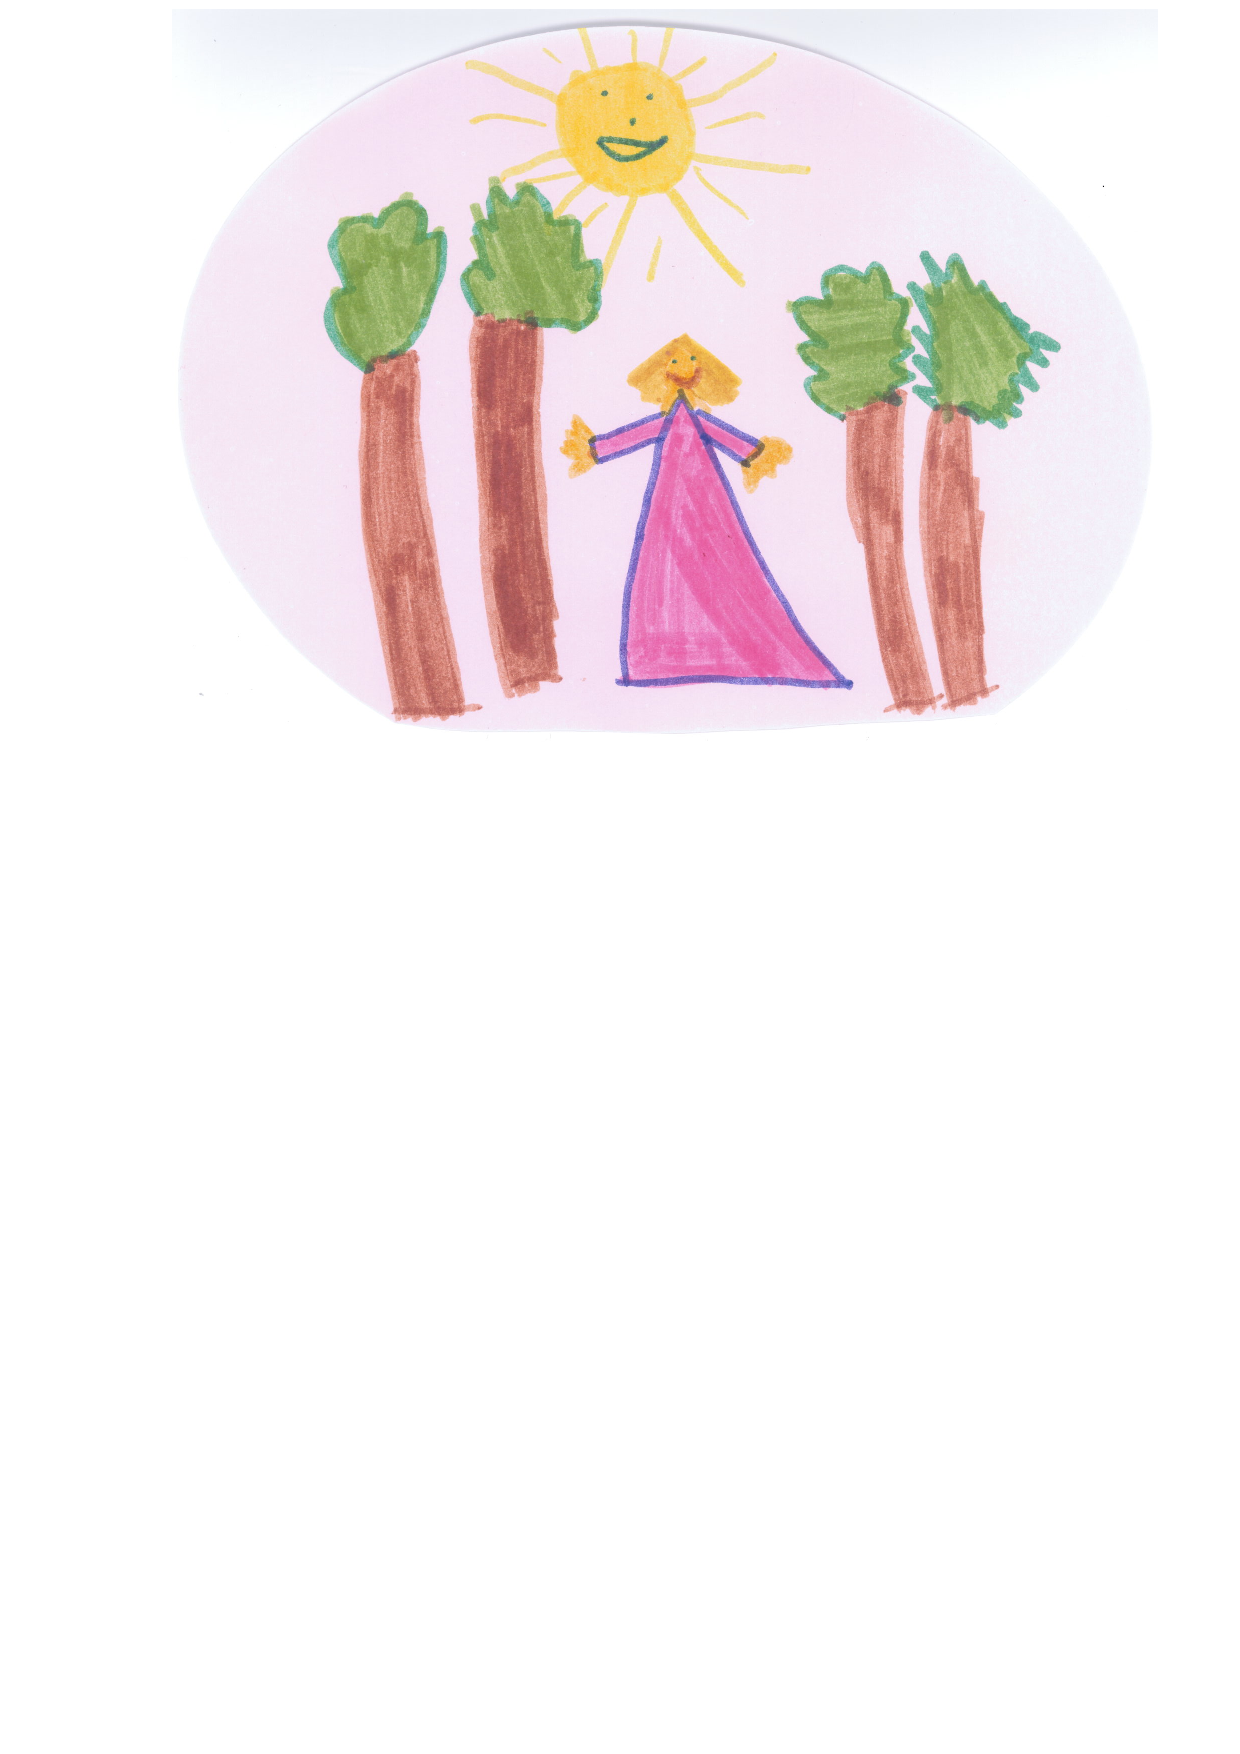
\includegraphics[width=.7\textwidth]{bilder/kerzers.pdf}
%\end{figure}

Mit einer Miene, die tiefen Ekel ausdrücken soll und ohne eine Antwort von Carla zu erwarten stapft die Dame davon. Ob sie weiss, dass gerade diese Schmetterlinge alle verschwunden sind, überlegt Carla?

Die beiden Schwestern treffen sich wie verabredet in der Cafeteria. Wie immer darf sich Carla nichts kaufen sondern muss das essen, was Fenja mitgebracht hat. Fenja erzählt kauend, dass man als nächstes bei den Sammlern und Züchtern nachfragen muss. Es sind im Moment die einzigen Verdächtigen. Und weil klar ist, dass sie hier nicht weiterkommen, beschliessen sie nach Bern zu fahren, an der Universität gibt es einen Spezialisten für Schmetterlinge. Das ist der, der neulich hier den Vortrag gehalten hat, am besten man fängt bei dem gleich an. Vielleicht hat der eine Ahnung, wer wohl ein Motiv hat, Schmetterlinge zu stehlen.
\begin{center}
\aldineleft
\end{center}

 Als sie in Bern ankommen, hat Fenja schon über das Internet herausgefunden, wie sie zur Universität kommen und wo sie dort den Schmetterlingsexperten finden. Dr.\,Adrìan Moreira heisst er, das Büro von ihm müssen sie jetzt suchen. \emph{Zoologisches Institut} steht über der Eingangstür. Als ob Fenja jeden Tag hier wäre, geht sie zielsicher zum Fahrstuhl und drückt den Knopf zum dritten Stock. Woher ihre Schwester wohl immer so genau weiss was zu tun ist, überlegt Carla.

\enquote{Hallo ich bin Adrìan} begrüsst sie ein junger Mann mit stark spanischem Akzent. Das verblüfft dann sogar Fenja. Sie hätte sich Professoren viel älter vorgestellt und das sagt sie ihm auch, um sicher zu gehen, dass sie mit dem richtigen spricht. Adrìan muss lachen. \enquote{Na erstens bin ich noch kein Professor und ausserdem seid ihr beiden ja auch nicht im typischen Alter von Detektivinnen.} Er schiebt den beiden je eine Dose Cola hin. Zu Hause dürfen sie die nie trinken, was aber jetzt natürlich keine der beiden stört. Nichts anmerken lassen, heisst es jetzt.

\enquote{Also, wie kann ich Euch helfen?} Fenja erklärt was passiert ist. Adrìan hört sehr aufmerksam zu.

\enquote{Nein. Da kann ich euch nicht helfen. Ich habe keine Ahnung, wer so etwas tun könnte. Aber halt, wartet einmal. Neulich war eine Dame hier, die hat sich genau für diesen Schmetterling interessiert. Und die wollte wissen, wie man es am besten schafft, dass die Flügel auch nach dem Tod der Schmetterlinge möglichst lange halten und ihr Blau behalten.}

\enquote{Wie heisst die Frau?} Fenja ist wie elektrisiert. Das ist die erste echte Spur. So etwas kann kein Zufall sein. Adrìan überlegt und schaut in seinem Computer nach.

\enquote{Ich befürchte, dass ich den nicht kenne. Ich glaube, die hat sich gar nie richtig vorgestellt. Aber ich kann sie euch beschreiben. Sie ist schon etwas älter, gross und wenn ihr mich fragt\dots} und statt etwas zu sagen tippt er sich mit dem Finger an die Stirn \enquote{Na jedenfalls hatte sie einen wirklich exzentrischen Hut auf. Riesig und mit Federn.} Jetzt ist Carla aufgeregt. 

\enquote{Die habe ich heute gesehen, im Papliliorama. Das ist die Frau, die die Kleider mit dem Schmetterlingsmuster gemacht hat!} Adrìan und Fenja sehen Carla verblüfft an. Carla erinnert sich, dass die Frau auch ihren Namen genannt hatte, aber den hat sie lengst vergessen. Namen kann sie sich einfach nicht merken. Und bevor Fenja böse ist, sagt sie lieber nicht, dass sie den Namen kennen sollte.

\enquote{Wie die heisst, weiss ich auch nicht, aber ich habe die Kleider fotografiert.} Adrìan und Carla blicken auf das Display des Fotoapparates. Fenja ruft derweil Herrn Butterblom an. Der weiss den Namen auch nicht auswendig, sieht aber schnell auf dem Schild unter dem ausgestellten Kleid nach. Studer-Matt heisst sie.

\enquote{Richtig}, ruft Carla, \enquote{jetzt fällt es mir auch wieder ein.} Fenja runzelt mit Blick auf ihre Schwester die Augenbrauen und schlägt aber ohne etwas zu sagen im Telefonbuch die Adresse nach. Mit kleinen Schwestern zu schimpfen lohnt sich nicht und den Namen haben sie ja jetzt auch so.

\enquote{Na ich komme mal besser mit.} sagt Adrìan.

Als sie bei Frau Studer-Matt ankommen, riecht es sehr verfault. Adrìan will an der Tür klingeln.

\enquote{Halt!} ruft Fenja. \enquote{Wenn die Schmetterlinge da drin sind, ist es besser wenn die Tür geschlossen bleibt. Die Schmetterlinge leben eigentlich in tropischen, also warmen Gebieten. Kalter Wind ist schädlich. Im Übrigen bin ich der Meinung, dass die Schmetterlinge sicher hier sind. Richt ihr nicht den Geruch? Das ist faulendes Obst, das Lieblingsessen des Blauen Morphofalters. Ich rufe jetzt Kommissarin Andermatt an, wir warten hier so lange.}

Adrìan ist verblüfft. Das hätte er eigentlich alles selber merken können. Hat er aber nicht. Zur Sicherheit bindet Fenja den Türknauf am Treppengeländer fest. So kann niemand von innen die Tür öffnen. Bei Verbrechern muss man vorsichtig sein! Eine Erfahrung, die Fenja schon häufiger gemacht hat. Genau wie immer ein paar Meter gelbe Schnur von Grossvater mit zu haben. Die war auch schon sehr oft nützlich. 

Eine halbe Stunde später ist die Kommisarin da. Sie hat auch gleich noch ein paar Kollegen mit gebracht, als Verstärkung. Sie klingeln jetzt doch an der Tür. Eine genervte Frau, die ganz offensichtlich tatsächlich Frau Studer-Matt ist, öffnet die Tür. Und auf ihrer Schulter sitzt auch schon der erste blaue Schmetterling.
\begin{center}
\aldineleft
\end{center}

Adrìan und Herr Butterblom fangen die Schmetterlinge in der Wohnung ein und bringen sie zurück ins Papiliorama. 

\enquote{Warum haben sie das getan?} Kommissarin Andermatt spricht die Frage aus, die alle brennend interessiert.

\enquote{Ich wollte, ich, \dots} Frau Studer-Matt kommt ins Stottern. Aber dann holt sie tief Luft und sagt: 

\enquote{Ich wollte das schönste und vollkommenste Kleid nähen, dass je ein Mensch getragen hat. Ich wollte es mit den Flügeln der Schmetterlinge besticken, den schönsten Pailletten der Welt. Das herrliche Blau dieser Schmetterlinge ist einfach unübertroffen. Das ist eine Erfindung, die so genial ist, dass vor mir noch niemand darauf gekommen ist. Ich werde vielleicht verhaftet, aber ich werde in die Modegeschichte eingehen. Das lasse ich mir auch nicht von euch Kleingeistern auch kaputt machen. Was sind schon ein paar Schmetterlinge gegen wahre Schönheit.}

Die Kommissarin schüttet den Kopf, Carla hat nicht ganz genau verstanden, was Frau Studer-Matt vor hatte und Fenja kann es sich nicht verkneifen zu erklären, dass schon früher Menschen in Süd- und Mittelamerika Kleider mit den Schalen von Käfern bestickt haben. Das ist nicht nur ganz ähnlich, sondern hält auch besser. 

Als die beiden Mädchen zu Hause ankommen, machen Mama und Papa geheimnisvolle Gesichter. 

\enquote{Na, habt ihr heute schön gespielt?} wollen sie wissen. Und noch während Fenja überlegt, ob man auch nicht schön spielen kann, zückt ihr Papa zwei Eintrittskarten hinter dem Rücken hervor.

\enquote{Überraschung: Morgen fahren wir alle zusammen nach Kerzers ins Papiliorama!} Da rufen die beiden Schwestern wie aus einem Mund:

\enquote{Oh nein, bloss nicht!} \hfill {\color{red}\decofourleft}


\chapter*{\FontH{\Huge Meine Freundin Henna}}
\addcontentsline{toc}{chapter}{Meine Freundin Henna}
\lettrine[lines=3]{\color{DeepPink}D}{as} mutigste Mädchen, das ich kenne, heisst Henna. Sie ist meine beste Freundin. Mit ihr kann man immer tolle Sachen erleben. Wollt ihr die spannendste Geschichte hören, die ich je mit ihr erlebt habe? Also gut, ich erzähle sie euch.

Alles begann damit, dass meine Tante Susanne etwas mit mir unternehmen wollte.
Susanne ist erst siebzehn Jahre alt und ziemlich cool. Keine meiner Freundinnen
hat eine so junge Tante. Von ihr weiss ich immer, welche Band gerade die beste
ist und was es bedeutet, die Tage zu haben.

Susanne hatte gerade furchtbaren Liebeskummer und wollte, wie sie sagte
\enquote{deswegen} mit mir ein Schloss besichtigen. Was Liebeskummer mit einem
Schloss zu tun haben könnte, weiss ich nicht, aber um ganz ehrlich zu sein, ich weiss schon nicht einmal, was Liebeskummer bedeuten soll. Das macht aber offenbar nichts, denn wenn mir Susanne von ihrem Liebeskummer erzählt, presse ich die Lippen zusammen, gucke so wie Papa, wenn er von seiner Arbeit spricht und nicke dazu. Susanne findet, dass ich die einzige bin, die sie versteht.

Und eine Freundin solle ich mal auch mitnehmen, hatte Susanne vorgeschlagen, dann werde es um so lustiger. Und damit hatte sie Recht. Bei so einer Einladung kam nur Henna in Frage. Da musste ich gar nicht lange überlegen. Wir drei vereinbarten, uns gegen späten Nachmittag beim Schloss zu treffen.

Schon gleich nach der Kasse begannen unsere Probleme, ohne das Henna und ich das aber wissen konnten. Ein junger Mann im Alter von Susanne stand hinter uns und irgendwie sind die beiden ins Gespräch gekommen. Die ersten beiden Räume, die wir im Schloss besichtigten, stand er die ganze Zeit neben uns. Die beiden waren sehr albern, viel alberner als wir. Dann entschuldigten sich er und Susanne, sie würden gerne einen Kaffee im Museum in der Nähe des Schlosses trinken gehen. Wir genehmigten gerne und machten uns auf den Weg durchs Schloss.

Das Schloss war wunderschön und könnte auch genauso in einem Märchenbuch gemalt worden sein. Hohe spitze Türme an allen Seiten, ringsherum ein Park, der mit einer hohen Mauer umgeben war. Wie bei einer Burg. Und überall Rosen. Die Zimmer waren laut Tafeln so, wie sie früher dann und dann gemäss der Phantasie des Schilderschreibers gewesen sein müssen. In jedem Zimmer ein Kachelofen und dann überall Rüstungen, Waffen und Besteck von damals. Wenn ich so ein Schloss gehabt hätte, hätte ich die Sachen wohl anders aufbewahrt, aber die Menschen früher haben sich wohl noch nicht so viele Gedanken gemacht wie wir jetzt. Das merke man schon daran, was sie für ein WC gehalten haben, meinte jedenfalls Henna, und da hatte sie Recht. Denn das WC war nur ein Erker in der Wand mit einem Loch. Henna und ich haben dort durchgespuckt und uns vorgestellt, was da sonst schon alles runtergefallen ist. Ob es wohl sehr umständlich war für einen Ritter, jedesmal die Rüstung abziehen zu müssen, wenn die hierher gekommen sind?

Wir sind in jedem Raum gewesen und haben uns immer eine Geschichte zu den Dingen überlegt, die da so standen. Henna meinte, dass die Menschen, die früher hier gelebt haben, noch an Zauberei, Drachen und Gespenster geglaubt haben. In einem Zimmer lag unter einer Vitrine ein sehr grosses aufgeschlagenes Buch, mit Buchstaben, die wir nicht lesen konnten. Das haben wir für ein Zauberbuch gehalten und uns gerade gefragt, ob das Buch selber zaubern kann oder ob man die Zaubersprüche erst vorlesen muss. Gerade als wir ausprobieren wollten, ob wir den ausgestopften Vogel in einem Regal wieder lebendig zaubern können, hörten wir ein lautes Krachen von draussen.

Eigenartigerweise war niemand mehr im Schloss zu sehen, als wir raus liefen, um
nach zu sehen. Auch im Park ist keine Menschenseele, dabei waren es noch so
viele, als wir gekommen waren. Das grosse Tor durch die Mauer ist zu. Eine
schwere Holztür ist da, wo wir rein gekommen sind. Das Schliessen des Tores hat
wohl den Krach gemacht, den wir gehört hatten, schlussfolgert Henna. Offenbar
ist das Museum geschlossen worden und wir hatten das verpasst. Wir waren
eingesperrt. Sofort fangen wir aus Leibeskräften an zu rufen. Aber niemand
hört. 

Henna unterbrach mich, es habe keinen Sinn so zu schreien. Auf ihren Rat hin liefen wir der Mauer entlang, um nachzusehen, ob wir nicht sonst irgendwo raus kommen, denn raus wollten wir hier. Das ist sicher. So eine Nacht in einem Schloss verbringen? Ganz alleine? Und wo war eigentlich Susanne? 

Aber da war kein anderes Tor und keine Lücke. Die Mauer war dicht, da kommt
niemand rein, dass haben die damals schon richtig gemacht, aber es kommt eben
auch niemand raus. Ich hatte plötzlich furchtbare Angst und eine Träne ist mir
über die Wange gelaufen. 

Henna nahm mich an die Hand, und zusammen sind wir wieder ins Schloss gegangen.
In jedem Schloss gebe es geheime Fluchtwege, meinte Henna. Man müsse nur in der
Bibliothek an einem bestimmten Buch ziehen, dann drehe sich die Wand und man
kommt in einen unterirdischen Tunnel. Das haben alle Schlösser, das kenne sie
aus dem Fernsehen.  Ich war zwar skeptisch, hatte aber keine bessere Idee. 

Also los und die Bibliothek suchen. Die Gänge entlang, Türen auf und wieder zu.
Aber nirgends eine Bibliothek. Die Ruhe in einem verlassenen Schloss ist
ziemlich unheimlich. Ausser dem Atmen von Henna ist nichts zu hören. Das dafür
aber besonders laut. Sie ist Allergikerin, wahrscheinlich waren gerade irgendwelche Pollen in der Luft. Noch schlimmer ist es bei Katzen. Katzenhaare merkt Henna sofort. Wenn ich die Katze von Susanne streichele und dann Henna besuche, muss sie sofort husten.

Es ist nicht nur still, sondern mit der Zeit auch dunkel geworden, denn die Sonne ging nun unter. Eine Rüstung hatte so einen langen Schatten geworfen, dass es aussah, als müsste irgendwo ein Riese stehen mit Schild und Schwert. Mir wurde es sehr flau im Magen, ich hatte ein bisschen Angst, denn Schlösser können, so schön sie am Tag auch sind, nachts ziemlich unheimlich werden. Deswegen werden die wohl auch abends geschlossen, nehme ich an. Ob Susanne überhaupt bemerkt hat, dass wir weg sind? Henna und ich versuchen einen Lichtschalter zu finden. Aber entweder sind die sehr gut versteckt, oder hier machen die noch Licht mit Kerzen. Jedenfalls suchten wir neben jeder Tür nach einem Schalter, zu Hause bei mir und bei Henna und bei jedem, den wir kennen, sind alle Lichtschalter neben einer Tür.

Ich überlegte gerade, wie das bei Onkel Tonis Stall ist, der ist auch ziemlich gross, so wie das Schloss und vielleicht ist das mit den Lichtschaltern ja anders in grossen Gebäuden. In dem Augenblick hörten wir einen Stock über uns ein leises Tapsen. Wäre es nicht so gruselig still gewesen und würde es in so einem Schloss nicht so hallen, hätten wir das nie gehört. Haben wir aber. Mir wäre fast das Herz in die Hose gerutscht und ich halte die Luft an, um bloss selber kein Geräusch zu machen. Erstens konnte ich so besser hören und zweitens konnte ich selber so nicht gehört werden. Auch Henna lauscht gespannt.

\afterpage{
    \begin{figure}
        \thispagestyle{empty}
        \centering
        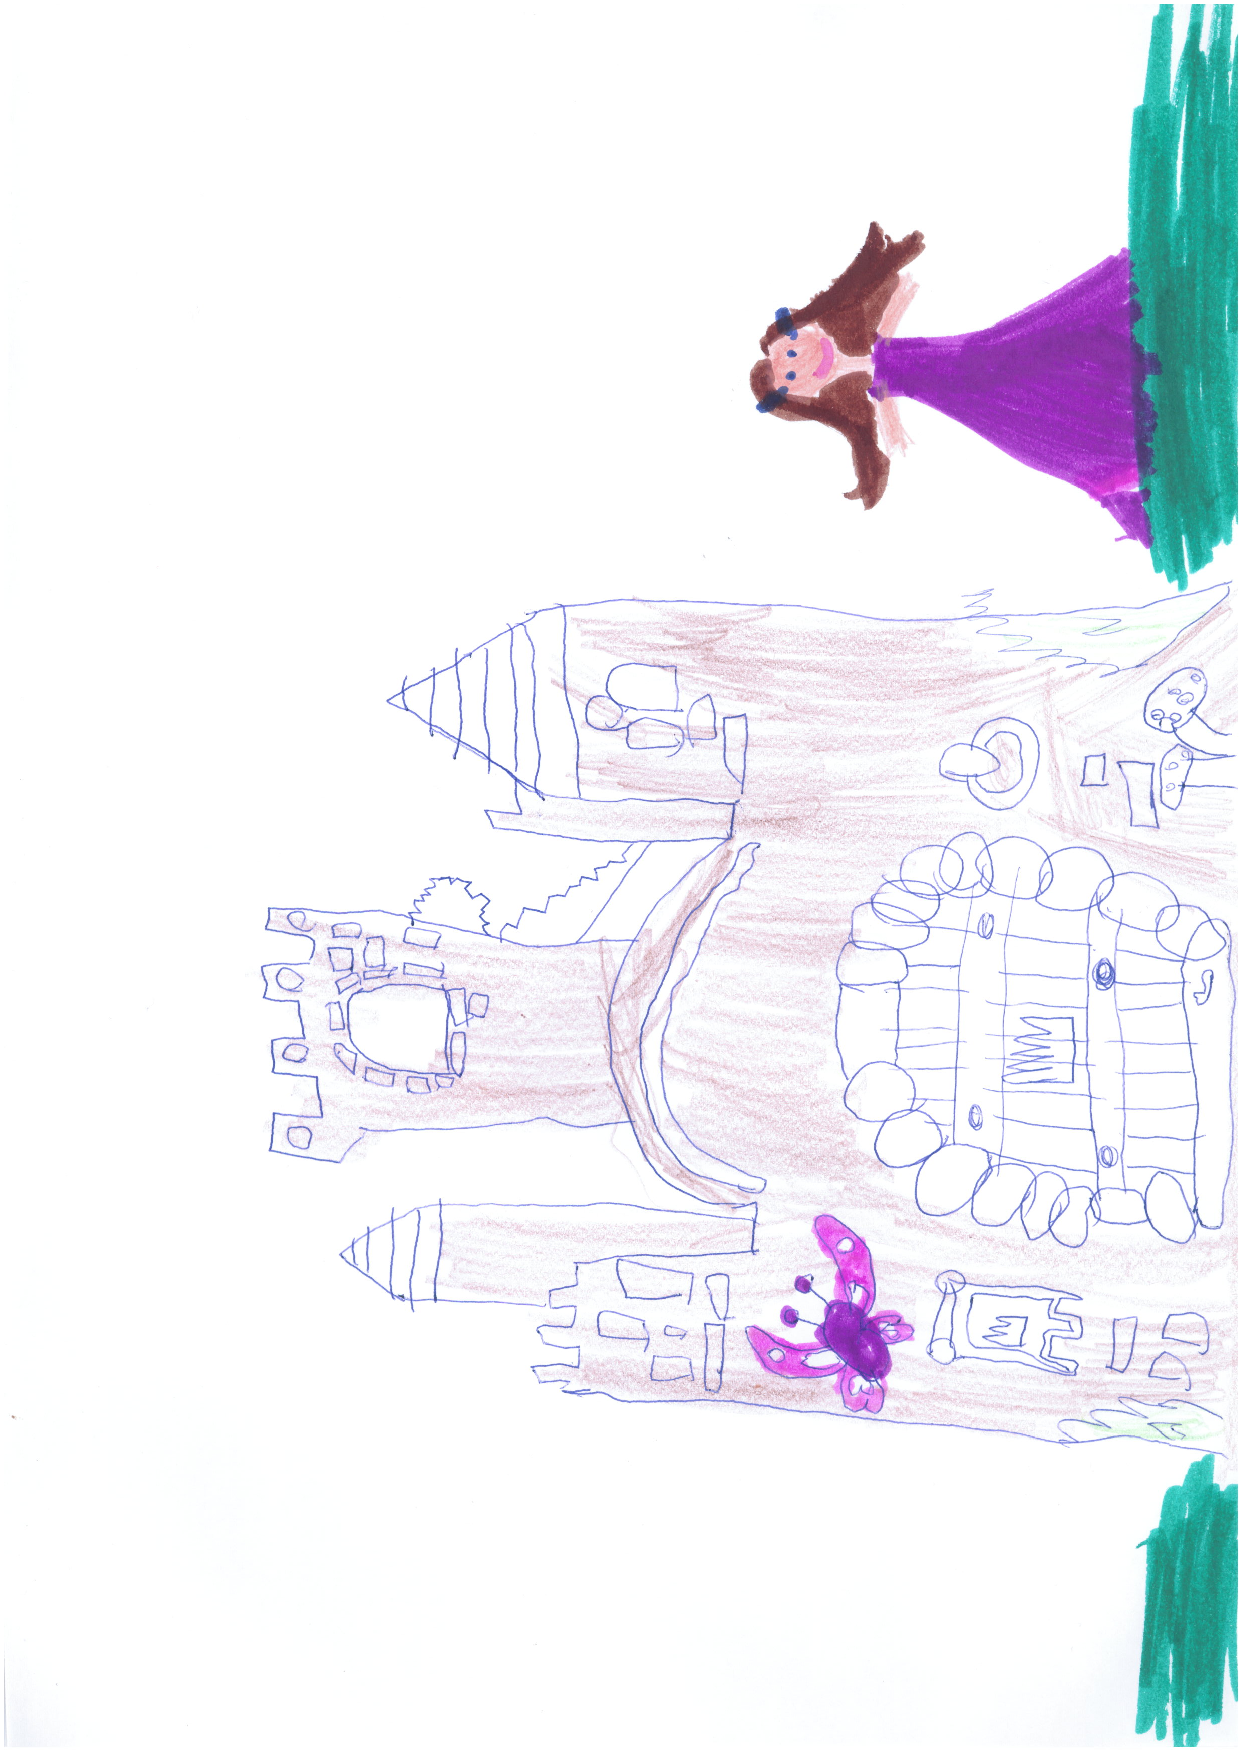
\includegraphics[width=\textwidth]{bilder/prinzessin.pdf}
    \end{figure}
    \clearpage
}

Was ist jetzt besser? Laut rufen, vielleicht ist da ja irgendwo Susanne und sucht uns oder lieber ganz leise sein und sich verstecken? Ich entschied mich gerade für die zweite Variante, denn wie von Susanne hat das Geräusch nicht geklungen. Na ja, das Geräusch hat eigentlich überhaupt nicht nach einem Mensch geklungen.

Aber Henna macht meinen Plan kaputt. Sie ruft ganz laut, ob da jemand sei. Ich
bin sehr erschrocken von der Lautstärke und von dem Echo. Niemand antwortet.
Henna ruft nochmals. Nichts. Doch dann war wieder das Tapsen zu hören. Henna
läuft sofort los um nachzusehen. Ich habe viel zu viel Angst, hier alleine
stehen zu bleiben, also folge ich ihr. Die Treppe hoch, dort kam das Geräusch
her. Mir bleibt fast das Herz stehen. Das Tapsen ist ganz klar aus dem Zimmer
am Ende des Ganges zu hören. Der Mond scheint sehr hell, es ist zwar alles zu
erkennen, aber nur schwarzweiss. Das ist mir da zum ersten Mal aufgefallen,
dass alle Dinge nachts grau werden. Henna geht zielstrebig auf das Zimmer zu.
Mein Herz schlägt so laut, als ob irgendjemand ganz laut Musik spielt. Ich bin
sicher, dass mindestens Henna das hören muss und wer immer da drin ist auch.
Wenn die Menschen, die hier gewohnt haben, an Gespenster geglaubt haben, dann hatten die womöglich doch Recht. Sind Gespenster eigentlich gefährlich? In Trickfilmen ja meistens nicht, aber ob man sich auf Trickfilme verlassen kann, ist ja wohl fraglich. Ich meine, da fallen ja auch sprechende Tieren Klaviere auf den Kopf und denen passiert nichts. 

Wir näherten uns dem Zimmer. Ich weiss nicht, warum genau wir eigentlich nachsehen wollten und ob es nicht besser gewesen wäre, sich zu verstecken und das wollte ich Henna auch gerade sagen, da ist sie schon in dem Zimmer und um die Ecke. Ich schnell hinterher. Das Tapsen kam vom anderen Ende des Zimmers. Der Mond schien durch das Fenster, aber um in jede Ecke zu gucken reichte das Licht nicht. Da ist es entweder ganz schwarz oder ein Wirrwarr aus Schatten, dass man nichts erkennen kann.

Plötzlich bewegte sich einer dieser Schatten und wird länger und immer länger
und so lang, dass er erst bis zur Wand hinter unserem Rücken reichte und dann
war ein lauter Schlag zu hören. Mir bleibt fast das Herz stehen. Tausende Scherben fliegen uns entgegen. Irgendetwas ist kaputt gegangen. So etwas wie eine riesige Tasse oder so, jedenfalls sahen die Scherben so aus.

Ich traute mich nicht einmal mit den Wimpern zu schlagen. Henna sprang aber nach vorne und greift zu. Ein Fauchen war zu hören. Ich konnte das alles nicht so richtig erkennen, aber ich hörte Henna rufen: \enquote{Übel, ganz übel \dots eine Katze!}

Und tatsächlich hielt sie eine Katze im Arm. Wie ihr euch vorstellen könnt, bin
ich noch nie im Leben so erleichtert gewesen, wie da. Kein Gespenst, kein Vampir, kein Einbrecher oder sonst etwas Schreckliches. Nie wäre ich auf die Idee gekommen, dass es eine Katze sein könnte! Henna sah das anders. Sofort fing sie an zu husten. Ich nahm ihr die Katze ab und scheuchte sie raus. 

Nachdem sich Henna ihre Hände gewaschen hatte, ging es mit dem Huste nauch
gleich besser. Ausserdem hatte sie ihr Spray dabei, dass sie sich in den Mund
gesprüht hatte. Dann ging es mit dem Husten auch gleich besser. 
 
Was wir dafür nicht mit hatten, war etwas zum Essen. Mir knurrte der Magen
mittlerweile so sehr, dass jede Angst im Schloss vergessen war. Das Bett der
Königin hat uns dann aber wieder versöhnt. Riesig und ein Himmelbett noch dazu.
Die Decke goldbestickt, aber etwas muffig. 

Dort haben wir gerade geübt, wer am höchsten springen kann und bis an die
Spitze des Himmelbetts kommt, als wir das Rufen von Stimmen hören. Die von
Susanne ist auch dabei und die von dem Typ auch. Schnell die Decke wieder gerade richten. Susanne entschuldigt sich tausend Mal, der Hausmeister will immer wieder wissen, ob wir etwas angefasst hätten und droht mit der Polizei, als er die umgestürzte Vase fand. Die Katzengeschichte will er uns nicht glauben, hier wäre noch nie eine Katze gewesen. Aber das ist jetzt alles nicht mehr unser Problem, dass muss jetzt wirklich Susanne lösen.

Wir vier gehen dann noch in eine Pizzeria und es wird noch ein sehr lustiger Abend. \hfill {\color{DeepPink}\decofourleft}





%\chapter*{\FontH{\Huge Aus dem Leben des Karl Rebosam}}
\addcontentsline{toc}{chapter}{Aus dem Leben des Karl Rebosam}
Karl ist auch in den Grundfragen der Pädagigik unorthodox. Je nach Vergehen des Zöglings schlägt sich Karl selbst ins Gesicht. Blut ist ein \emph{must}. Das soll dem Knaben eine Lehre sein!

Gelegentlich ertappt sich Karl bei dem Gedanken, sein Kind zur Adoption frei zu geben.
\begin{center}
{\huge \textthing}
\end{center}
Karl ist heute sehr nachdenklich. Er hatte folgenden Algorithmus angewendet:
\begin{enumerate}
	\item Öffne das Telefonbuch.
	\item Bilde die Quersumme der Telefonnummer des ersten Eintrags beim Buchstaben \emph{A}.
	\item Notiere das Ergebnis und verfahre so bei allen weiteren Buchstaben.
	\item Addiere alle Ergebnisse und bilde die Quersumme.
	\item Bilde aus diesem Wert so lange die Quersumme, bis diese einstellig ist.
	\item Wiederhole alle vorhergehenden Schritte für den jeweils letzten Eintrag eines Buchstabens.
\end{enumerate}
Das Ergebnis erwies sich in beiden Fällen als $5$. Was hat das zu bedeuten? Voll innerlicher Welkeheit schritt Karl seine Sammlung ausgestopfter Nagetiere ab und empfand es einmal mehr als schmerzlich, dass ausgerechnet eine Ratte noch nicht zu integrieren gewesen war.
\begin{center}
{\huge \textthing}
\end{center}
An jedem achten Tag nach Neumond empfand Karl Rebosam Lust. Schon der Anblick der morgentlichen Zahnpasta, wie sie sich schlangenfraugleich aus der Tube auf seine Bürste windet und er diese dann in seinen Mund schiebt und nach einem kurzen Augenblick des Innhaltens sanft aber kräftig mit der Zunge zerdrückt, liess heissen Schweiss aus seiner Stirn triefen. 

Und wenn dann der  Toaster durch die Behandlung mit feuriger Glut aus zwei bleichen schwammigen Fladen, braune knusprige Wesen erschafft und diese mit einem Knall aus seinem inneren heraus spuckt, ist Karl der Ohnmacht jeweils schon recht nahe.
\begin{center}
{\huge \textthing}
\end{center}
Es stellte sich als kapitalen Fehler heraus, das falsch gegebene Rückgeld zu reklamieren. Die Bäckersfrau war nicht bereit, Kritik zu akzeptieren. Diese kategorische Charaktereigenschaft, gepaart mit einer Meisterschaft in der Schwitzkastentechnik, führten zu einer für Karl nicht vorhersehbaren Reaktion.

Karl verbrachte einen wesentlichen Teil des Vormittags unter der Achselhöle der sonst frommen Bäckersfrau. Er musste mit Respekt beobachten, wie die Bedienung der ihm nachfolgenden Kundschaft ganz reibungslos durch die Vermittlung nur eines Arms funktionierte. Im Grunde klappe sie sogar besser als mir beiden Armen, denn da Katls Gesicht beim Bezahlen jeweils tief in die Kasse gedrückt wurde, konnte er bei der Herausgabe des Wechselgeldes mitzählen. Ein weiterer Fehler war dabei der Bäckersfrau nicht vorzuwerfen. Ärgerlich war im Weiteren nur, dass er seine Pfeife nicht mitgenommen hatte.
\begin{center}
{\huge \textthing}
\end{center}
Heute hat Karl folgende annonce im Lokalblatt publizieren lassen: {\it Hundesalon Rebosam sucht per sofort einen Hundecoiffeur. Neben viel Libe zu den Vierbeinern erwarten wir einen männlichen Berwerber, der aus Gründen der Authenzität möglichst selbst stark behaart ist. Ausnahmen gelten nur für Träger eines Menjou oder eines Dali-Bärtchens. Weitere Auskunft erhalten sie unter Tel. \ldots. }

Natürlich gibt es diesen Hundesalon Rebosam gar nicht. Die Telefonnummer ist aber tatsächlich die unseres Karln.
\begin{center}
{\huge \textthing}
\end{center}
\hfill {\color{red}\decofourleft}


%Inhaltsverzeichnis
\newpage
\tableofcontents

\end{document}



